\documentclass[12pt,openany]{ctexbook}

\usepackage[a4paper,margin=2.4cm]{geometry}
\usepackage{amsmath,amssymb,mathtools}
\usepackage{amsthm}
\usepackage{bm}
\usepackage{booktabs,longtable,tabularx,array,multirow}
\usepackage{graphicx}
\usepackage{subcaption}
\usepackage{float}
\usepackage{tikz}
\usepackage{pgfplots}
\usepackage{hyperref}
\usepackage[capitalise]{cleveref}
\usepackage{enumitem}
\usepackage{listings}
\usepackage{xcolor}
\usepackage{xurl}
\usepackage{microtype}

\pgfplotsset{compat=1.18}
\hypersetup{colorlinks=true,linkcolor=blue,citecolor=blue,urlcolor=blue}
\setlist[itemize]{nosep}
\setlist[enumerate]{nosep}
\setlength{\LTleft}{0pt}
\setlength{\LTright}{0pt}
\raggedbottom

% 定理环境
\newtheorem{theorem}{定理}[chapter]
\newtheorem{lemma}[theorem]{引理}
\newtheorem{proposition}[theorem]{命题}
\newtheorem{corollary}[theorem]{推论}
\theoremstyle{definition}
\newtheorem{definition}[theorem]{定义}
\newtheorem{example}[theorem]{例}
\theoremstyle{remark}
\newtheorem{remark}[theorem]{注}

% cleveref 中文支持
\crefname{theorem}{定理}{定理}
\crefname{lemma}{引理}{引理}
\crefname{proposition}{命题}{命题}
\crefname{corollary}{推论}{推论}
\crefname{definition}{定义}{定义}
\crefname{example}{例}{例}
\crefname{remark}{注}{注}

\title{石器时代战斗系统与宠物养成机制的源码还原与定量分析}
\author{Rode (QQ:81881788)}
\date{\today}

\DeclareRobustCommand{\code}[1]{\ifmmode\text{\nolinkurl{#1}}\else\nolinkurl{#1}\fi}
\newcommand{\vstd}{\ensuremath{(V,S,T,D)}}
\newcommand{\dex}{\ensuremath{\mathrm{DEX}}}
\newcommand{\atk}{\ensuremath{\mathrm{ATK}}}
\newcommand{\defn}{\ensuremath{\mathrm{DEF}}}
\newcommand{\luck}{\ensuremath{\mathrm{LUCK}}}
\newcommand{\fixdex}{\code{WORKFIXDEX}}
\newcommand{\quick}{\code{WORKQUICK}}
\newcommand{\attdex}{\ensuremath{att_{\mathrm{dex}}}}
\newcommand{\defdex}{\ensuremath{def_{\mathrm{dex}}}}

\begin{document}

\frontmatter
\maketitle

\chapter*{摘要}
本文基于 \code{gmsv} 源码，建立石器时代战斗系统与宠物养成机制的统一定量模型。研究内容包括：(1)~变量符号体系与源码口径的规范化映射；(2)~行动顺序、命中回避、会心反击、法术命中等战斗概率公式的源码还原；(3)~属性场地、四属性结界、属性反转等动态机制的状态转移分析；(4)~宠物成长、转生、融合、蛋喂养流程与战斗能力的映射关系；(5)~基于离散优化的宠物培养策略建模。本文采用源码还原、分段函数推导、状态转移分析与数值实验相结合的方法，将玩家经验转化为可验证的定量结论，为战斗配装与目标导向优化提供理论基础。

\vspace{1em}
\noindent\textbf{关键词：}石器时代；战斗系统；宠物成长；源码分析；离散优化

\tableofcontents

\mainmatter
\chapter{绪论}

\section{研究背景与问题来源}

石器时代这类运行时间很长的网络游戏，往往会在玩家群体中沉淀出大量经验说法。它们有的来自长期实战观察，有的来自旧版私服口径，有的则是在不同版本、不同分支、不同翻译文本之间不断转述后形成的“近似共识”。这类经验说法并非没有价值，但它们通常存在三个问题：第一，只描述现象，不明确变量进入公式的顺序；第二，把局部成立的经验外推到全局；第三，忽略取整、上限和状态更新顺序带来的离散跳变。对石器时代而言，这三个问题几乎正好覆盖了宠物养成与战斗系统最容易争议的部分。

本研究直接缘起于一类反复出现的具体问题：宠物转生后的成长上下限为什么会出现经验上“超模”或“不到位”的情况；融合和蛋喂药到底何时取整、何时压缩；战斗中的乱敏、命中、会心、结界、属性反转和骑宠攻防到底看哪一层属性。若只看玩家经验，这些问题往往只能得到零散回答；但若直接回到源码，则有机会把它们统一到同一套变量和状态转移框架下分析。也正因为如此，本文不把战斗系统和宠物养成系统分开研究，而是试图把两者接成一条完整的因果链。

\section{研究目标}

本文的目标可以概括为四点。第一，建立统一的变量与符号体系，使玩家口径、工具口径和源码变量能够一一对应。第二，还原战斗系统中的关键定量机制，包括乱敏、回避、命中、会心、法术命中、场地、结界、属性加强、属性反转以及骑宠伤害。第三，把宠物成长、转生、融合、蛋喂药和孵化过程纳入同一分析框架，并说明它们如何继续影响高等级战斗属性。第四，在机制还原的基础上，把若干典型玩家问题重新表述为可计算的离散优化问题。

更进一步说，本文并不满足于“说明某个公式是什么”，而是希望回答“该公式的变量如何影响结果”“哪些经验判断只在局部成立”“哪些最优化直觉会被取整和上限破坏”。因此，全文会反复强调变量进入顺序、边界条件和分段结构，而不把系统误写成连续线性的近似模型。

\section{研究方法}

本文以当前持有的 \code{gmsv} 源码为主要依据，并以项目 \code{sa_pet_assistant} 中已经对齐源码的工具实现作为辅助验证环境。具体方法包括：

第一，\emph{源码还原}。对关键函数、状态变量和宏展开做逐段阅读，确认公式结构、状态更新顺序和取整位置。第二，\emph{符号化整理}。把散落在不同文件与不同函数中的变量映射到统一符号体系，尽量减少章节之间的口径漂移。第三，\emph{分段函数推导}。对乱敏、命中、会心、伤害和喂药压缩等机制写出可分析的分段函数。第四，\emph{状态转移分析}。对场地、结界、属性加强、属性反转等动态状态，用“写入-读取-衰减-覆盖”的视角理解其演化。第五，\emph{数值与图形辅助}。对部分关键公式生成热力图或切片图，用于展示变量影响与局部非单调现象。第六，\emph{优化建模}。将融合蛋喂药等问题形式化为整数约束下的目标优化问题。

本文采取的总体原则是保守和可验证。对于源码中未明确实现或尚未验证完全的机制，本文只给出保守描述，而不依赖经验去补全“应该如此”的公式。这样做虽然会牺牲部分叙述上的圆满性，但能保证结论与代码口径尽可能一致。

\section{本文结构}

全文结构如下。第 2 章建立研究对象、符号与源码口径；第 3 章和第 4 章分别讨论宠物基础成长模型，以及转生、融合、蛋喂药与孵化链条；第 5 章和第 6 章整理战斗有效属性、状态变量与乱敏机制；第 7 章和第 8 章讨论物理概率与法术命中；第 9 章研究属性系统的动态变换；第 10 章给出骑宠、攻防混合与物理伤害公式；第 11 章把宠物成长映射回战斗能力；第 12 章把相关问题形式化为优化模型并讨论案例；第 13 章总结全文并指出后续工作。

整体上，本文遵循“先统一口径，再还原机制，最后做优化分析”的顺序。这种结构安排的出发点很直接：如果没有前面的变量口径和离散规则，后面的最优化结论就无法判断究竟是在优化源码，还是只是在优化某种近似直觉。


\chapter{研究对象、符号与源码口径}

本章为全文建立统一语言。石器时代的玩家经验、工具页面、源码变量和数学符号存在差异,需要统一澄清。本文将人物、宠物、骑宠、蛋与战斗状态置于同一符号体系下,并显式说明随机、取整与上下限的作用位置。

\section{研究对象与版本口径}

本文研究对象包括五类：人物、宠物、骑宠状态下的人物--宠物组合、融合蛋，以及战斗中的敌方单位。这些对象的机制相互关联：宠物成长档位影响战斗敏捷，骑宠状态混合人物与宠物的攻防敏属性，蛋喂药和孵化通过成长率映射到命中、回避、会心和伤害。

本文的主要源码依据是当前项目的 \code{gmsv} 代码树及其配套文档。对于已验证的机制,本文直接给出公式；对于尚未完全核实的机制,在正文中标记为”待进一步校核”。在骑宠、职业技能与属性状态系统相关部分,编译开关会改变具体实现,全文默认采用当前项目已核对的主要口径：骑宠三围与战斗伤害以 \code{_BATTLE_NEWPOWER} 分支为主,必要时指出 \code{_BACK_VERSION} 的参与情况。

本文构建的是对当前源码口径自洽、可计算、可验证的数值模型,而非还原”所有可能的服务器实现”。后文若无特别说明,”成立””等于””上限””下限”等表述均指”在当前 \code{gmsv} 源码与编译路径下成立”。

\section{统一符号体系}

本文采用表~\ref{tab:global-symbols} 和表~\ref{tab:battle-symbols} 所示的统一符号体系。表~\ref{tab:global-symbols} 列出成长与对象记号,表~\ref{tab:battle-symbols} 列出战斗概率记号；完整符号索引、别名与源码变量对应关系见附录~A。

在记号选择上,宠物基础成长档统一记作 $\bm{g}$,蛋基础成长统一记作 $\bm{b}$,孵化后成长统一记作 $\bm{h}$。玩家常用的 \vstd{} 在正文中作为玩家口径别名出现,不与 $\bm{g}$ 并列为主记号。

\begin{table}[H]
    \centering
    \caption{全局核心符号与成长相关记号}
    \label{tab:global-symbols}
    \begin{tabularx}{\linewidth}{@{}>{\raggedright\arraybackslash}p{2.5cm} >{\raggedright\arraybackslash}p{3.0cm} X@{}}
        \toprule
        记号 & 含义 & 说明 \\
        \midrule
        $V,S,T,D$ & 宠物四项成长率 & 分别对应生命、攻击、防御、敏捷方向的成长来源 \\
        $\bm{g}$ & 基础成长档 & 正文主记号；玩家口径常把它写成 \vstd{} \\
        $VSTD$ & 四项成长和 & 定义为 $V+S+T+D$ \\
        $L_v$ & 宠物等级 & 用于区分蛋、孵化后宠物、转生前宠物等阶段 \\
        $\bm{b}$ & 蛋基础成长 & 融合完成后、喂药前或喂药后的蛋面值 \\
        $\bm{h}$ & 孵化后成长 & 不含出生后额外随机加点的孵化结果 \\
        \shortstack[l]{$\mathrm{HP}, \mathrm{ATK},$\\$\mathrm{DEF}, \mathrm{SPD}$} & 宠物面板四围 & 分别表示界面中显示的生命、攻击、防御、敏捷数值 \\
        $x_1,x_2,x_3,x_4$ & 线性目标函数权重 & 用于喂药优化、养成反推等问题 \\
        \bottomrule
    \end{tabularx}
\end{table}

\begin{table}[H]
    \centering
    \caption{战斗核心符号与概率记号}
    \label{tab:battle-symbols}
    \begin{tabularx}{\linewidth}{@{}>{\raggedright\arraybackslash}p{2.5cm} >{\raggedright\arraybackslash}p{3.0cm} X@{}}
        \toprule
        记号 & 含义 & 说明 \\
        \midrule
        \attdex & 攻击方固定敏 & 在玩家 PVP 简化模型中通常对应 \fixdex{} \\
        \defdex & 防守方固定敏 & 在玩家 PVP 简化模型中通常对应防守方 \fixdex{} \\
        $L$ & 幸运修正 & 依上下文代表攻方或守方幸运，玩家有效范围通常为 $1\sim 5$ \\
        $C$ & 武器会心值 & 源码中的武器会心附加参数 \\
        $F$ & 反击武器系数 & 玩家反击率中的武器对武器系数 \\
        $\alpha,\beta,\gamma$ & 概率参数 & 分别对应回避、会心、反击公式中的主参数 \\
        $p_{\mathrm{duck}}$ & 普通回避率 & 不含独立前判的普通闪避概率 \\
        $p_{\mathrm{hit}}$ & 普通命中率 & 通常定义为 $100\%-p_{\mathrm{duck}}$ \\
        $p_{\mathrm{crit}}$ & 会心率 & 当前为普通物理会心判定 \\
        $p_{\mathrm{counter}}$ & 反击率 & 在满足反击前提后的成功概率 \\
        \bottomrule
    \end{tabularx}
\end{table}

在战斗层面，本文特别区分两类敏捷变量。其一是 \fixdex{}，可理解为”这回合用于命中、回避、会心、反击等概率判定的固定敏”；其二是 \quick{}，可理解为”这回合真正用于行动顺序计算的速度敏”。在大多数情况下，\quick{} 由 \fixdex{} 经过战斗修正后生成，但并不总是与后者相等。因此，后文若讨论命中、回避或会心，优先使用”固定敏”；若讨论乱敏、先手与速度档，则优先使用”战斗速度敏”。

\section{术语约定}

为保证全文表述的一致性与可追溯性，本文采用三层并行的术语映射规则：

\begin{description}[leftmargin=2.5cm,style=nextline]
\item[\textbf{源码层}] 使用 \code{WORKFIXDEX}、\code{WORKQUICK}、\code{BATTLE\_COM\_GUARD} 等源码标识符，保持与 \code{gmsv} 代码的字面一致性。源码层表述主要出现在需要精确定位实现细节的场合。

\item[\textbf{数学层}] 使用 $\attdex$、$\defdex$、$p_{\mathrm{duck}}$、$\bm{g}$ 等数学符号，用于公式推导与定量分析。数学层符号与源码变量的对应关系见附录~A。

\item[\textbf{语义层}] 使用”固定敏””战斗速度敏””普通回避率””咒术动作分支”等中文术语，用于解释机制含义与玩家理解。语义层表述优先采用玩家社区的通用说法，但会在首次出现时明确其源码对应。
\end{description}

正文中优先使用数学符号进行推导，必要时在括号内注明源码标识或语义说明。例如：”攻击方固定敏 $\attdex$ (对应源码变量 \fixdex{})”。对于动作类型与状态标记，优先使用源码标识并附语义解释，例如：”\code{BATTLE\_COM\_JYUJYUTU} (咒术动作分支)”。

\section{随机、取整与上下限}

战斗与宠物系统的争议主要源于三个位置：随机发生位置、截断发生位置、上限施加位置。本节按这三个层次说明。

\subsection{随机宏的整数性质}

源码中频繁使用随机宏：
\begin{equation}
    \operatorname{RAND}(x,y) = (x-1)+1+\left\lfloor \frac{(y-(x-1))r}{RAND\_MAX+1} \right\rfloor,
\end{equation}
其中 $r$ 为区间 $[0,RAND\_MAX]$ 上的随机整数。关键性质是其\emph{输出恒为整数}。无论出现在蛋喂药、升级成长、乱敏、命中附加、伤害抖动还是状态触发中,随机结果在进入后续公式前已回到整数域。

\subsection{截断而非四舍五入}

源码中大量百分比计算以浮点形式出现,但目标变量为整数,赋值时发生截断。例如
\begin{equation}
    \attdex^{\prime}=\lfloor 0.8\,\attdex \rfloor, \qquad \defdex^{\prime}=\lfloor 0.6\,\defdex \rfloor,
\end{equation}
以及
\begin{equation}
    d' = \lfloor 0.9 d \rfloor.
\end{equation}
凡涉及 $0.8$、$0.6$、$0.9$ 等身份修正、状态修正或百分比修正,若最终回写到整数变量,均为向下截断而非四舍五入。对宠物成长与蛋喂药问题,离散截断改变最优方案的边界(见第~\ref{chap:optimization-and-cases}~章定理~\ref{thm:feed-boundary})；对战斗概率问题,截断改变临界敏捷差和阈值位置。

\subsection{裁切算子的统一表示}

为统一书写上限与下限,定义裁切算子
\begin{equation}
    \operatorname{clip}_{[a,b]}(z) = \min\{\max\{z,a\},b\}.
\end{equation}
例如,在玩家 PVP 的简化回避模型中,普通回避率可写为
\begin{equation}
    p_{\mathrm{duck}}(\attdex,\defdex,L) = \operatorname{clip}_{[0.01,75.00]}\!\bigl(d_{\mathrm{base}}(\attdex,\defdex)+L\bigr),
\end{equation}
会心率可写为
\begin{equation}
    p_{\mathrm{crit}}(\attdex,\defdex,L,C) = \operatorname{clip}_{[0.01,100.00]}\!\bigl(c_{\mathrm{base}}(\attdex,\defdex,C)+L\bigr).
\end{equation}
该写法将”基础体”和”上限效应”分离。后文做偏导和单调性分析时,先分析基础函数,再讨论被裁切区间内导数变为零的情形。

\subsection{需要特别留意的三个离散位置}

全文中需要谨慎处理的离散点有三类。第一类是\emph{身份修正},例如人物打宠物、宠物打敌人时的 $0.6$ 或 $0.8$ 缩放；第二类是\emph{成长压缩与上限},例如宠物单项成长上限和总和上限；第三类是\emph{概率裁切},例如 $75\%$ 的回避上限和 $100\%$ 的会心上限。它们共同决定一个重要事实：玩家直觉中的”边际收益连续变化”在真实系统中不成立,经常出现平台、跳变和局部非单调区间。

\section{源码变量与游戏文本映射}

为兼顾源码准确性与玩家可读性,表~\ref{tab:code-game-map} 整理\emph{不提前解释易误读正文}且偏”动作语义/状态语义”的源码标识。\code{WORKFIXDEX}、\code{WORKQUICK}、\code{WORKFIXLUCK} 等通用工作值已在附录~A 中完整定义,不在本表重复。

\begin{table}[H]
    \centering
    \caption{高频源码动作 / 状态与玩家语义映射}
    \label{tab:code-game-map}
    \begin{tabularx}{\textwidth}{>{\raggedright\arraybackslash}p{0.30\textwidth} >{\raggedright\arraybackslash}p{0.18\textwidth} X}
        \toprule
        源码标识 & 玩家口径 & 说明 \\
        \midrule
        \code{BATTLE_COM_GUARD} & 防御 & 当前动作为防御时，普通闪避函数最前面直接失败 \\
        \code{BATTLE_COM_JYUJYUTU} & 咒术动作分支 & 名称对应日文“咒术”的罗马字写法；当前主要覆盖人物法术、魔法道具与部分宠技；不是防御；若防守方当前动作是该分支，普通回避参数改为 $0.027$ \\
        \code{CHAR_BATTLEFLG_NODUCK} & 不能闪避 & 一旦存在，该单位无法通过普通回避公式闪避 \\
        \code{CHAR_BATTLEFLG_AIBAD} & 本回合忠诚失控标记（nono） & 由宠物忠诚检查临时置位，表示本回合没有按玩家原指令行动 \\
        \code{CHAR_BATTLEFLG_REVERSE} & 属性反转状态 & 作用层级需结合具体公式分析，是第~\ref{chap:dynamic-attr} 章重点之一 \\
        \code{CHAR_WORKBATTLECOM3} & 动作附加参数槽 & 高 16 位与低 16 位在不同动作下含义不同 \\
        \bottomrule
    \end{tabularx}
\end{table}

其中,\code{CHAR_WORKBATTLECOM3} 需要特别说明。它不是单一含义的数值,而是”当前动作的附加参数寄存槽”。在职业技能中,常以”高 16 位存技能等级、低 16 位存阵列或子类型”形式出现；在法术和法术道具中,又改为”低位存法术编号,高位存等级或附加参数”。脱离当前动作编号而单独解读 \code{CHAR_WORKBATTLECOM3} 易造成误判。

综上,本文采用”源码标识 + 数学符号 + 玩家语义”三层并行写法：需要精确时使用源码标识,需要推导时使用数学记号,需要解释时回到玩家语言。这样既保证公式严谨,也保证章节之间顺畅衔接。

\chapter{宠物基础数值模型}

本章的目标是回答一个基础但决定性的问題：玩家在界面中看到的宠物属性，究竟是如何由宠物的成长率生成的。若不先把这一层关系写清楚，后文关于转生、融合、蛋喂药与战斗表现的讨论就会失去共同基础。与很多玩家的直觉不同，宠物的 \vstd{} 并不会直接决定最终面板，而是先经过随机波动、档位判定、出生初始化、升级随机与显示公式，最后才表现为生命、攻击、防御与敏捷。

\section{宠物 \vstd{} 与成长率的关系}

在本文中，宠物的基础成长方向由四维向量
\begin{equation}
    \bm{g}=(V,S,T,D)
\end{equation}
表示，其中四个分量分别对应生命、攻击、防御与敏捷方向的成长率。对应的总和记为
\begin{equation}
    VSTD = V+S+T+D.
\end{equation}
需要强调的是，$VSTD$ 在研究中非常重要，但它本身并不是一个足以完全描述宠物的量。两只宠物即使具有相同的 $VSTD$，只要四维分配不同，其成长方向和实战表现也可能差异明显。因此，全文在大多数地方都同时保留“总和视角”和“分量视角”。

当前项目中，宠物原始成长点数到显示属性的换算可整理为
\begin{equation}
    HP = \left\lfloor \frac{4V_r + S_r + T_r + D_r}{100} \right\rfloor,
\end{equation}
\begin{equation}
    ATK = \left\lfloor \frac{S_r + 0.1T_r + 0.1V_r + 0.05D_r}{100} \right\rfloor,
\end{equation}
\begin{equation}
    DEF = \left\lfloor \frac{T_r + 0.1S_r + 0.1V_r + 0.05D_r}{100} \right\rfloor,
\end{equation}
\begin{equation}
    SPD = \left\lfloor \frac{D_r}{100} \right\rfloor,
    \label{eq:pet-display-map}
\end{equation}
其中 $(V_r,S_r,T_r,D_r)$ 代表进入显示公式之前的原始累计点数，而不是输入页面上的基础成长率本身。式~\eqref{eq:pet-display-map} 说明了四项成长率之间并非完全隔离：$V$ 主要影响生命，但也会少量进入攻击和防御；$D$ 主要影响敏捷，但同样会少量影响攻击和防御。因此，单纯以“主属性”理解宠物仍然不够，真正的映射关系是一个带交叉项的线性变换再叠加整数截断。

从数学上看，这一映射具有两个重要特点。第一，它是\emph{多对一}的：不同的原始点数组合，在通过向下取整之后，可能得到相同的显示属性。第二，它是\emph{层级式}的：显示属性不是直接由 $(V,S,T,D)$ 得到，而是由后续随机过程累积出的 $(V_r,S_r,T_r,D_r)$ 得到。也正因为如此，所谓“由显示属性反推成长率”天然只能得到候选集，而不能总是得到唯一解。

\section{等级、成长与初始化随机}

\subsection{一级初始化的三步结构}

对普通宠物而言，一级初始化并不是把基础成长率直接乘上某个系数，而是包含三步。第一步是四维独立的 $\pm2$ 波动：
\begin{equation}
    \varepsilon_i \in \{-2,-1,0,1,2\}, \qquad g_i^{(s)} = g_i + \varepsilon_i,
\end{equation}
其中 $g_i^{(s)}$ 表示真正存入成长档的“生效成长率”。第二步是用波动后的四项和判定 Rank，而不是用基础输入的 $VSTD$ 判定。第三步是在出生时进行一次总计 $10$ 点的随机分配，每次随机给四维中的某一项加 $1$。当前项目配套的宠物成长模拟，为了与既有模拟口径保持一致，在这一步额外采用了“单项最多额外得到 $4$ 点”的限制；这里需要特别说明，这一条是\emph{工具侧模拟设定}，不是本文已从服务器源码中直接验证出的硬编码上限。若按“$10$ 次独立、每次以 $1/4$ 概率落到某一维”的无上限模型看，对预先指定的一项有
\begin{equation}
    X \sim \mathrm{Binomial}(10, 1/4), \qquad
    \Pr(X \ge 5) = \sum_{k=5}^{10} \binom{10}{k} (1/4)^k (3/4)^{10-k} \approx 7.81\%.
\end{equation}
进一步地，$\Pr(X \ge 6) \approx 1.98\%$，$\Pr(X \ge 7) \approx 0.35\%$。因此，“单项超过 $4$ 点”在无上限随机模型下并非理论不可能，只是对某一指定维度而言概率不高。若将出生时随机加点记作 $e_i$，初始化参数记作 $INITNUM$，则一级原始点数满足
\begin{equation}
    g_{r,i}^{(1)} = INITNUM \cdot \bigl(g_i^{(s)} + e_i\bigr).
    \label{eq:lv1-raw}
\end{equation}
式~\eqref{eq:lv1-raw} 说明，一级面板已经同时混合了“基础成长率”“$\pm2$ 波动”“出生随机加点”和“初始化尺度”四类信息。

\subsection{0 转宠与转生宠的 Rank 判定差异}

Rank 是宠物成长系统中的关键中介变量，但它并不是对所有宠物共用同一张表。当前源码与工具口径下，至少要区分两类对象：其一是普通宠物，也就是玩家常说的“0 转宠”；其二是已经经过转生流程、重新进入成长路径的转生宠。两者虽然都会在后续成长中使用 Rank，但用于判定 Rank 的总和门槛并不相同。

对于普通宠物，Rank 由波动后的 $VSTD$ 判定，其分界如表~\ref{tab:normal-rank} 所示。

\begin{table}[H]
    \centering
    \caption{普通宠物（0 转宠）的 Rank 判定表}
    \label{tab:normal-rank}
    \begin{tabular}{cc}
        \toprule
        波动后 $VSTD$ & Rank \\
        \midrule
        $\ge 100$ & 0 \\
        $\ge 95$  & 1 \\
        $\ge 90$  & 2 \\
        $\ge 85$  & 3 \\
        $\ge 80$  & 4 \\
        $<80$      & 5 \\
        \bottomrule
    \end{tabular}
\end{table}

对于转生宠，Rank 判定门槛会发生变化，其分界如表~\ref{tab:trans-rank} 所示。

\begin{table}[H]
    \centering
    \caption{转生宠的 Rank 判定表}
    \label{tab:trans-rank}
    \begin{tabular}{cc}
        \toprule
        波动后 $VSTD$ & Rank \\
        \midrule
        $\ge 130$ & 0 \\
        $\ge 100$ & 1 \\
        $\ge 95$  & 2 \\
        $\ge 85$  & 3 \\
        $\ge 80$  & 4 \\
        $<80$      & 5 \\
        \bottomrule
    \end{tabular}
\end{table}

这两张表的差异意味着：同样是一个波动后的成长总和，放在 0 转宠和转生宠身上，不一定会落到相同 Rank。尤其是 Rank 0 的门槛从 $100$ 提高到 $130$，直接改变了高成长转生宠的判定标准。因此，任何把“普通宠的 Rank 规则”直接套用到转生宠上的分析，都会在后续成长倍率、随机区间和分布判断上产生系统性偏差。

从结构上说，Rank 的判定对象始终是“波动后的生效成长总和”，而不是输入页上的理想成长率总和；但判定所用的门槛表，会随着宠物是否已经转生而变化。后文第 4 章讨论转生模型时，会进一步说明：首转在计算原宠 Rank 时仍使用普通表，而转生后的新成长率在继续进入成长流程时，应按转生宠的 Rank 表理解。

Rank 一经确定，就会进入升级随机的倍率表。当前实现中，不同 Rank 对应的随机倍率区间如表~\ref{tab:frand-ranges} 所示。

\begin{table}[H]
    \centering
    \caption{不同 Rank 的升级倍率范围}
    \label{tab:frand-ranges}
    \begin{tabular}{cc}
        \toprule
        Rank & $fRand$ 对应整数区间 \\
        \midrule
        0 & $[450,500] \times 0.01$ \\
        1 & $[470,520] \times 0.01$ \\
        2 & $[490,540] \times 0.01$ \\
        3 & $[510,560] \times 0.01$ \\
        4 & $[530,580] \times 0.01$ \\
        5 & $[550,600] \times 0.01$ \\
        \bottomrule
    \end{tabular}
\end{table}

这组区间表明，Rank 并不是一个“纯评价标签”，而是后续升级过程中的随机参数入口。也就是说，同一只基础宠物如果因为 $\pm2$ 波动跨过了 Rank 边界，后续升级整条路径都会被改写。

\subsection{0 转宠与转生宠的完整成长口径对照}

玩家常说“0 转和转生后的宠物档位设置不同”。若按源码精确定义，这句话应理解为：两者真正不同的是 Rank 判定门槛及其进入点，而不是整个成长引擎都换了一套。一级初始化公式、出生 $10$ 点随机、升级时的 $10$ 点随机、$fRand$ 倍率表，以及最终显示公式，本质上仍是同一套结构；发生变化的是“用哪张 Rank 表解释波动后的成长总和”。这一点可整理为表~\ref{tab:normal-vs-trans-growth}。

\begin{table}[H]
    \centering
    \caption{0 转宠与转生宠的成长口径对照}
    \label{tab:normal-vs-trans-growth}
    \begin{tabularx}{\textwidth}{>{\raggedright\arraybackslash}p{3.6cm} >{\raggedright\arraybackslash}X >{\raggedright\arraybackslash}X}
        \toprule
        比较项目 & 0 转宠 & 转生宠 \\
        \midrule
        适用对象 & 普通捕捉宠、普通孵化宠、尚未进入转生路径的宠物 & 已完成转生并重新进入成长流程的宠物 \\
        Rank 判定对象 & 波动后的生效成长总和 $\sum_i g_i^{(s)}$ & 波动后的生效成长总和 $\sum_i g_i^{(s)}$ \\
        Rank 门槛 & 使用表~\ref{tab:normal-rank}：Rank 0 门槛为 $100$ & 使用表~\ref{tab:trans-rank}：Rank 0 门槛提高到 $130$ \\
        一级出生 $10$ 点随机 & 总计 $10$ 点；当前工具模拟默认额外采用单项最多 $4$ 点的限制 & 同左 \\
        升级时 $10$ 点随机 & 总计 $10$ 点，不设单项 $4$ 点限制 & 同左 \\
        $fRand$ 区间表 & 使用表~\ref{tab:frand-ranges} & 与 0 转宠相同，仍使用表~\ref{tab:frand-ranges} \\
        显示属性换算 & 使用式~\eqref{eq:pet-display-map} & 与 0 转宠相同，仍使用式~\eqref{eq:pet-display-map} \\
        \bottomrule
    \end{tabularx}
\end{table}

表~\ref{tab:normal-vs-trans-growth} 的意义在于，它把“档位设置不同”这件事拆成了“哪些变量真的改了，哪些步骤其实没改”。如果不做这一步区分，读者很容易误以为转生后连出生随机、升级随机甚至显示公式都一起改变；但从当前源码和工具实现看，这些部分并没有改动，真正变动的是 Rank 的解释规则，因此受影响最直接的是后续 $fRand$ 抽样区间的选择。

这里还需要额外区分两个容易混淆的 Rank 场景。第一，\emph{转生公式内部}为了计算 $F_x$，需要先给“原宠”判一次 Rank：首转使用普通表，二转使用转生表。第二，\emph{转生完成之后}，由转生公式生成的新成长率 $\bm{g}^{(new)}$ 再进入正常成长流程时，应把它视为“转生宠”，因此后续 $\pm2$ 波动后的 Rank 判定统一按转生表处理。前者服务于转生能力值公式本身，后者服务于转生后新宠的出生与升级随机，这两层 Rank 虽然名字相同，但作用阶段并不相同。

\subsection{升级随机模型}

在每次升级时，系统还会再做两件事。其一是重新进行一次总和为 $10$ 的随机加点，但这一次不再有“单项最多 $4$ 点”的限制；其二是根据 Rank 所对应的区间抽取一次倍率 $fRand$。若第 $\ell$ 级到第 $\ell+1$ 级的随机加点记为 $p_i^{(\ell)}$，则升级增量满足
\begin{equation}
    \Delta g_{r,i}^{(\ell)} = \left\lfloor \bigl(g_i^{(s)} + p_i^{(\ell)}\bigr) fRand^{(\ell)} \right\rfloor.
    \label{eq:levelup-delta}
\end{equation}
因此，高等级宠物的最终属性并不是某个固定点，而是一个分布。式~\eqref{eq:levelup-delta} 也解释了为什么项目中的成长模拟输出分位数而不是单值：在完整随机机制下，“最弱”“中位”“最强”本来就是不同样本路径的产物，而非同一路径中的不同观测角度。

\section{单项上限、总和上限与压缩机制}

从研究视角看，宠物系统中的上限可以分成两类。第一类是\emph{随机模型侧约束}，例如当前配套模拟在普通宠一级初始化时，对出生 $10$ 点随机分配额外施加的“单项最多 $4$ 点”限制；第二类是\emph{成长档压缩约束}，例如后文在蛋喂药、孵化和融合过程中会反复出现的单项上限与总和上限。前者主要影响初始点的离散分布，后者则直接改变成长档本身。

对普通成长模拟而言，最重要的结论是：出生随机加点不会改写已经存档的成长率，它只改变一级原始点数和之后的面板起点。与之相对，蛋喂药和孵化中的压缩会改变进入后续成长过程的成长档，因此它的影响会贯穿整个生命周期。也正因为此，后文在讨论养成优化时总是把“孵化后成长”视为真正的优化目标，而不是蛋基础成长或出生后一时的面板数值。

从数学上说，带上限的系统通常不是连续最优化问题，而是离散约束优化问题。无论是单项上限、总和上限，还是“先平均再乘系数”“先乘系数再取整”的顺序差异，都会造成可行域的折角与跳点。对宠物工具而言，这意味着搜索算法比闭式公式更重要；对论文而言，这意味着必须把上限发生的位置写清楚，否则所谓“某个方案更优”的结论就缺乏口径基础。

\section{蛋面数值与孵化后数值的关系}

融合与喂药系统引入了“蛋基础成长”和“孵化后成长”这两个容易混淆的概念。本文记蛋基础成长为
\begin{equation}
    \bm{b}=(b_V,b_S,b_T,b_D),
\end{equation}
它表示融合完成后、喂药前或喂药后的蛋面数值；再记孵化后成长为
\begin{equation}
    \bm{h}=(h_V,h_S,h_T,h_D),
\end{equation}
它表示按孵化公式折算之后、但尚未进入出生后 10 点随机加点之前的成长档。当前工具中，优化问题和大多数比较都以 $\bm{h}$ 为对象，而不是以一级显示属性为对象。

在无喂药情形下，当前实现中的确定性孵化模型可看作以 $\bm{b}$ 为输入、以 $\bm{h}$ 为输出的整数映射；而在有喂药情形下，还要先经过药效折算、单项裁切、总和压缩和按比例回分配等步骤，详见下一章。无论是否喂药，都必须区分“孵化后成长”和“出生后状态”：前者是进入成长流程的成长档，后者还会叠加后续的 $\pm2$ 波动、Rank 判定和出生随机加点。

因此，蛋面数值与孵化后数值之间的关系并不是“输入即输出”，而是“蛋面成长作为中间状态，经过一套带取整和上限的孵化映射后，生成真正参与后续成长的成长档”。从建模角度看，这一层正是把融合、喂药和普通成长统一起来的关键接口。后文关于转生、融合与喂药的所有公式，最终都会回到本章建立的两层结构：一层是成长档，另一层是由成长档驱动的随机成长过程。

\chapter{宠物养成机制：转生、融合与蛋喂养}

如果说上一章回答的是“宠物怎样长”，那么本章回答的是“宠物怎样被改造”。在当前系统中，转生、融合和蛋喂药并不是彼此独立的补丁，而是一条连续的养成流水线：原宠可以先通过转生改变成长档结构，也可以通过融合生成蛋基础成长，再经喂药与孵化映射为新的成长档，最终重新进入普通成长过程。因此，本章的重点不只是逐个介绍规则，而是把这些规则写成可组合的离散模型。

\section{转生模型}

\subsection{转生输入与总体结构}

转生模块的输入包括原宠成长率 $\bm{g}=(g_1,g_2,g_3,g_4)$、MM 向量 $\bm{m}=(m_1,m_2,m_3,m_4)$、宠物等级 $L_v$、转生次数以及转生能力上限。当前工具中，首转默认上限为 $150$，二转默认上限为 $200$，但这一上限允许人工覆盖，因此在论文中将其统一记为参数 $A_{\max}$。

转生并不是直接给出高等级宠物的最终面板，而是先生成一组新的基础成长率，再让该成长率像普通宠物一样经历后续出生与升级流程。若将转生后的确定性成长率记作 $\bm{g}^{(new)}$，则转生的逻辑链为
\begin{equation}
    (\bm{g},\bm{m},L_v,\text{转生次数},A_{\max})
    \longrightarrow A
    \longrightarrow \bm{g}^{(new)}
    \longrightarrow \text{普通成长流程}.
\end{equation}
其中 $A$ 即当前实现中的转生能力值，对应项目内部变量 \code{ans}。

\subsection{Rank、Fx 与转生能力值}

设原宠总和为
\begin{equation}
    T_2 = \sum_{i=1}^4 g_i,
\end{equation}
MM 总和经上限裁切后为
\begin{equation}
    T_1 = \min\left\{\sum_{i=1}^4 m_i,\,150\right\}.
\end{equation}
首转时，原宠 Rank 按普通宠物的 Rank 表判定；二转时，则改按转生宠 Rank 表判定。记此 Rank 为 $r$，则项目实现中的
\begin{equation}
    F_x = \left\lfloor (5-r)\times 1.2 \right\rfloor + 5.
\end{equation}
将等级截到 $130$ 以内，记
\begin{equation}
    \tilde{L} = \min\{L_v,130\},
\end{equation}
则转生能力值可整理为
\begin{equation}
    A = \left\lfloor 1.3\left(\frac{T_1}{100}\right)^5 \right\rfloor + T_2 + \left\lfloor \frac{\tilde{L}-100}{F_x} \right\rfloor.
    \label{eq:trans-ans-raw}
\end{equation}
再施加转生能力上限，得到
\begin{equation}
    A^{*} = \min\{A,A_{\max}\}.
    \label{eq:trans-ans-cap}
\end{equation}
式~\eqref{eq:trans-ans-raw} 和式~\eqref{eq:trans-ans-cap} 共同说明了三个事实：第一，MM 总和的作用不是线性叠加，而是通过五次方项提供高阶放大；第二，等级补正只在 $100$ 级之后发挥作用，并且在 $130$ 级后不再继续增长；第三，最终增长永远受上限控制，因此转生能力值不可能无限增大。

\begin{figure}[H]
    \centering
    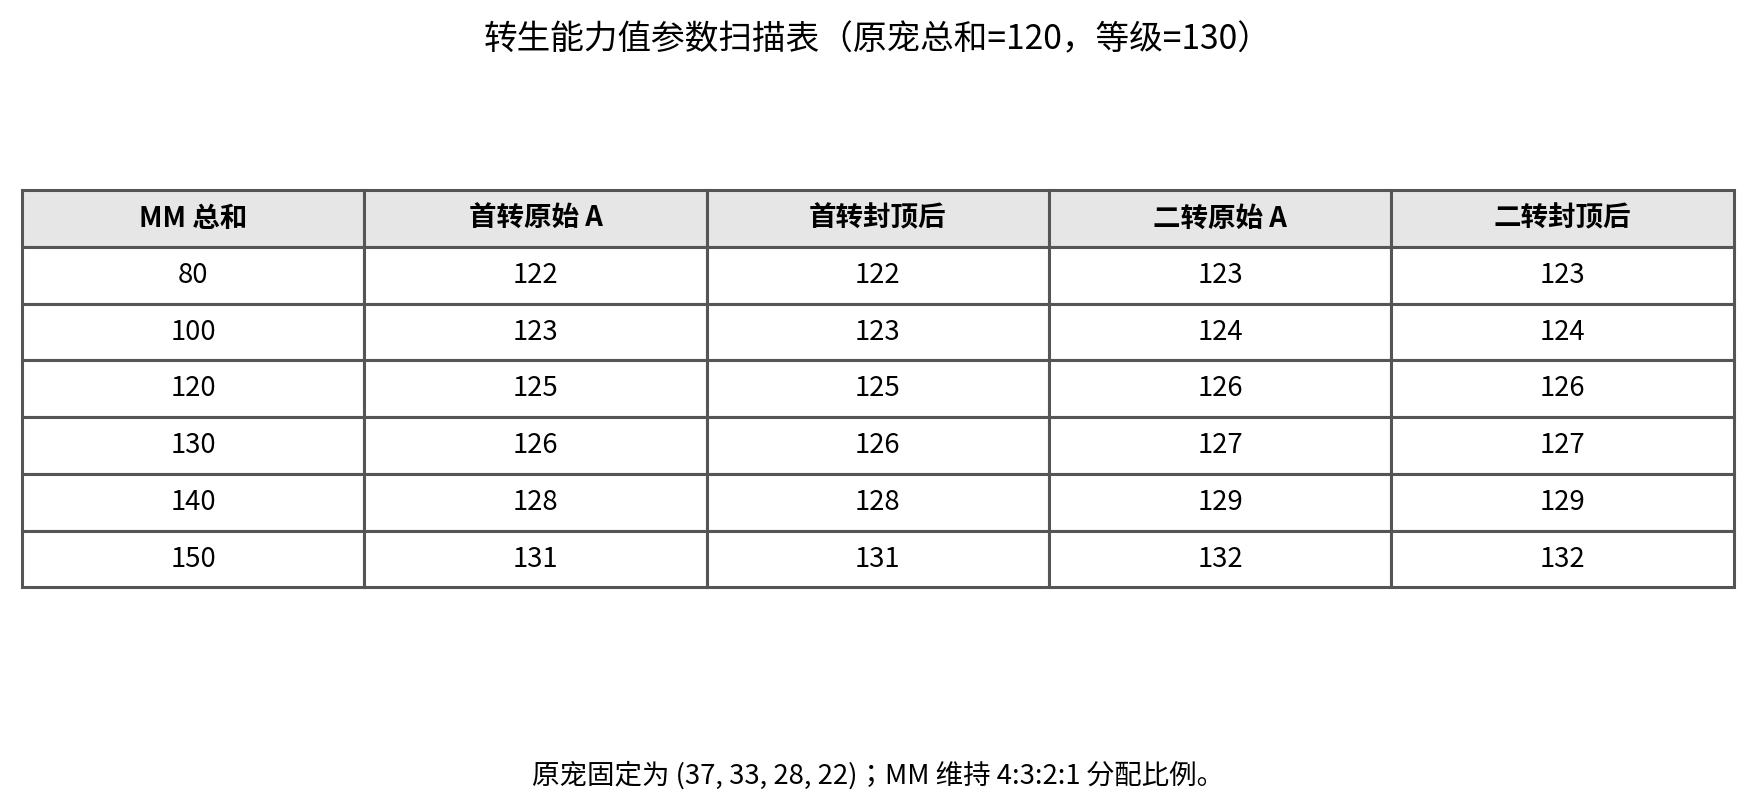
\includegraphics[width=0.82\textwidth]{figures/transmigration_scan_table.png}
    \caption{转生能力值参数扫描表。固定原宠成长总和为 $120$、宠物等级为 $130$，并令 MM 的四维分配保持 $4{:}3{:}2{:}1$ 比例。表中同时列出首转与二转的原始转生能力值和上限裁切结果，用于展示 Rank 表差异与能力上限的共同影响。}
    \label{fig:trans-scan-table}
\end{figure}

式~\eqref{eq:trans-new-alloc} 本身也是一个离散分配器，因为四维结果都分别向下取整，所以分配后的四项总和一般小于 $A^{*}$。这种“能力值存在，但落不到任何一维”的现象，正是转生页面中经常出现 1 至 3 点落差的根源。图~\ref{fig:trans-alloc-loss-table} 给出一个固定原宠与 MM 配置下的实证扫描，可以看到即使 $A^{*}$ 继续上升，四维总和也会以台阶方式增长，而不是逐点连续增长。

\begin{figure}[H]
    \centering
    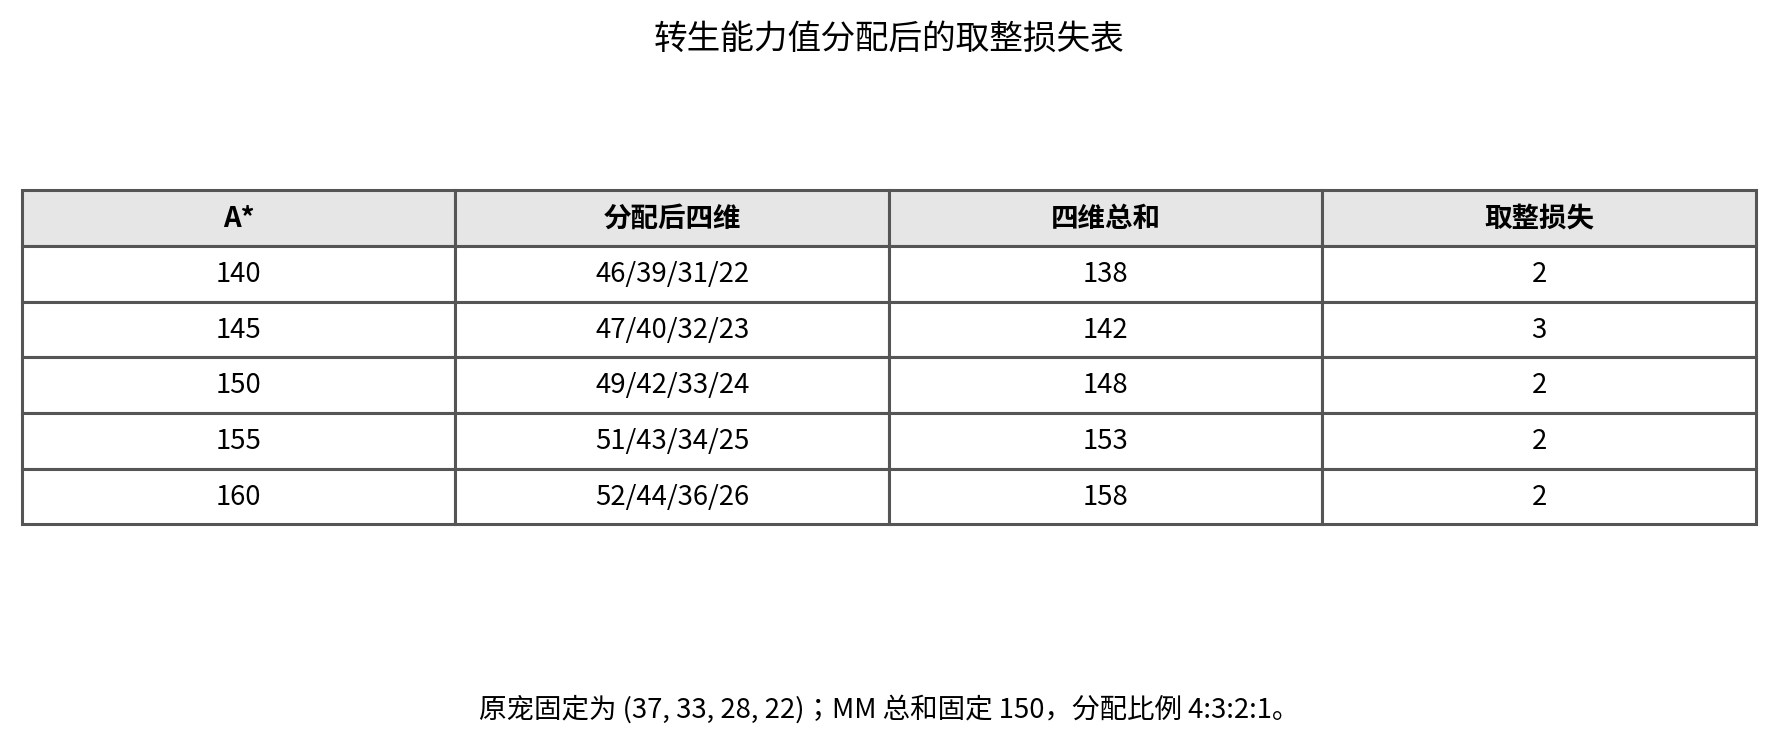
\includegraphics[width=0.82\textwidth]{figures/transmigration_alloc_loss_table.png}
    \caption{转生能力值分配后的取整损失表。固定原宠成长为 $(37,33,28,22)$、MM 总和为 $150$ 且分配比例为 $4{:}3{:}2{:}1$，展示不同 $A^{*}$ 在按权重分配并逐项向下取整后，四项总和与原能力值之间的差额。}
    \label{fig:trans-alloc-loss-table}
\end{figure}

\subsection{按权重分配到四项成长}

得到 $A^{*}$ 之后，系统并不会把它平均分到四维，而是按“原宠四倍权重、MM 一倍权重”的方式重新分配。记总权重为
\begin{equation}
    W = T_1 + 4T_2,
\end{equation}
则每一维的新成长率为
\begin{equation}
    g_i^{(new)} = \left\lfloor \frac{A^{*}(m_i + 4g_i)}{W} \right\rfloor, \qquad i=1,2,3,4.
    \label{eq:trans-new-alloc}
\end{equation}
式~\eqref{eq:trans-new-alloc} 解释了为什么 MM 更像“修方向”而不是“推翻原宠结构”：在同样的 $A^{*}$ 下，原宠原本偏向哪一维，新的成长档仍会显著保持这种偏向。

最后还必须强调，$\bm{g}^{(new)}$ 只是转生后的\emph{确定性基础成长率}，而不是最终宠物。它仍会经历上一章中的 $\pm2$ 波动、Rank 判定、出生随机加点和升级随机。因此，转生后的高等级属性依旧是一组分布，而不是单点。

\section{融合模型}

\subsection{主宠、副宠与低等级折扣}

融合模块的输入包括主宠与一只或两只副宠的等级及成长率。若某只参与融合的宠物等级低于 $80$，则其四维成长在进入后续步骤之前，需要先逐项做低等级折扣：
\begin{equation}
    g_i' = \left\lfloor 0.8 g_i \right\rfloor.
    \label{eq:fusion-level-discount}
\end{equation}
这里的关键不是 $0.8$ 这个系数本身，而是它\emph{先于后续贡献系数发生}。也就是说，主宠并不是“先乘 $0.6$ 再统一乘 $0.8$”，副宠也不是“先平均后再看是否低于 $80$ 级”，而是每只低等级宠物先单独完成一次截断，再进入主宠贡献或副宠平均的后续步骤。

\subsection{主宠贡献与副宠贡献}

设主宠折扣后的成长向量为 $\bm{g}^{(M)}$，副宠折扣后的成长向量分别为 $\bm{g}^{(S1)}$、$\bm{g}^{(S2)}$。若副宠数量为 $n_s\in\{1,2\}$，则先求逐项和
\begin{equation}
    s_i = \sum_{k=1}^{n_s} g_i^{(Sk)},
\end{equation}
再逐项做整数平均
\begin{equation}
    \bar{s}_i = \left\lfloor \frac{s_i}{n_s} \right\rfloor.
    \label{eq:sub-avg}
\end{equation}
随后，主宠贡献与副宠贡献分别为
\begin{equation}
    c_i^{(M)} = \left\lfloor 0.6 g_i^{(M)} \right\rfloor,
\end{equation}
\begin{equation}
    c_i^{(S)} = \left\lfloor 0.4 \bar{s}_i \right\rfloor.
    \label{eq:sub-contrib}
\end{equation}
最终蛋基础成长为
\begin{equation}
    b_i = c_i^{(M)} + c_i^{(S)}.
    \label{eq:egg-base}
\end{equation}
式~\eqref{eq:sub-avg} 与式~\eqref{eq:sub-contrib} 的顺序非常重要，因为“先平均再乘 $0.4$”与“先乘 $0.4$ 再平均”在整数系统中并不等价。当前实现与 \code{gmsv} 一致，明确采用前者。因此，融合模型本质上是一个逐步取整的离散算子，而不是一个可任意交换次序的线性组合。

\begin{figure}[H]
    \centering
    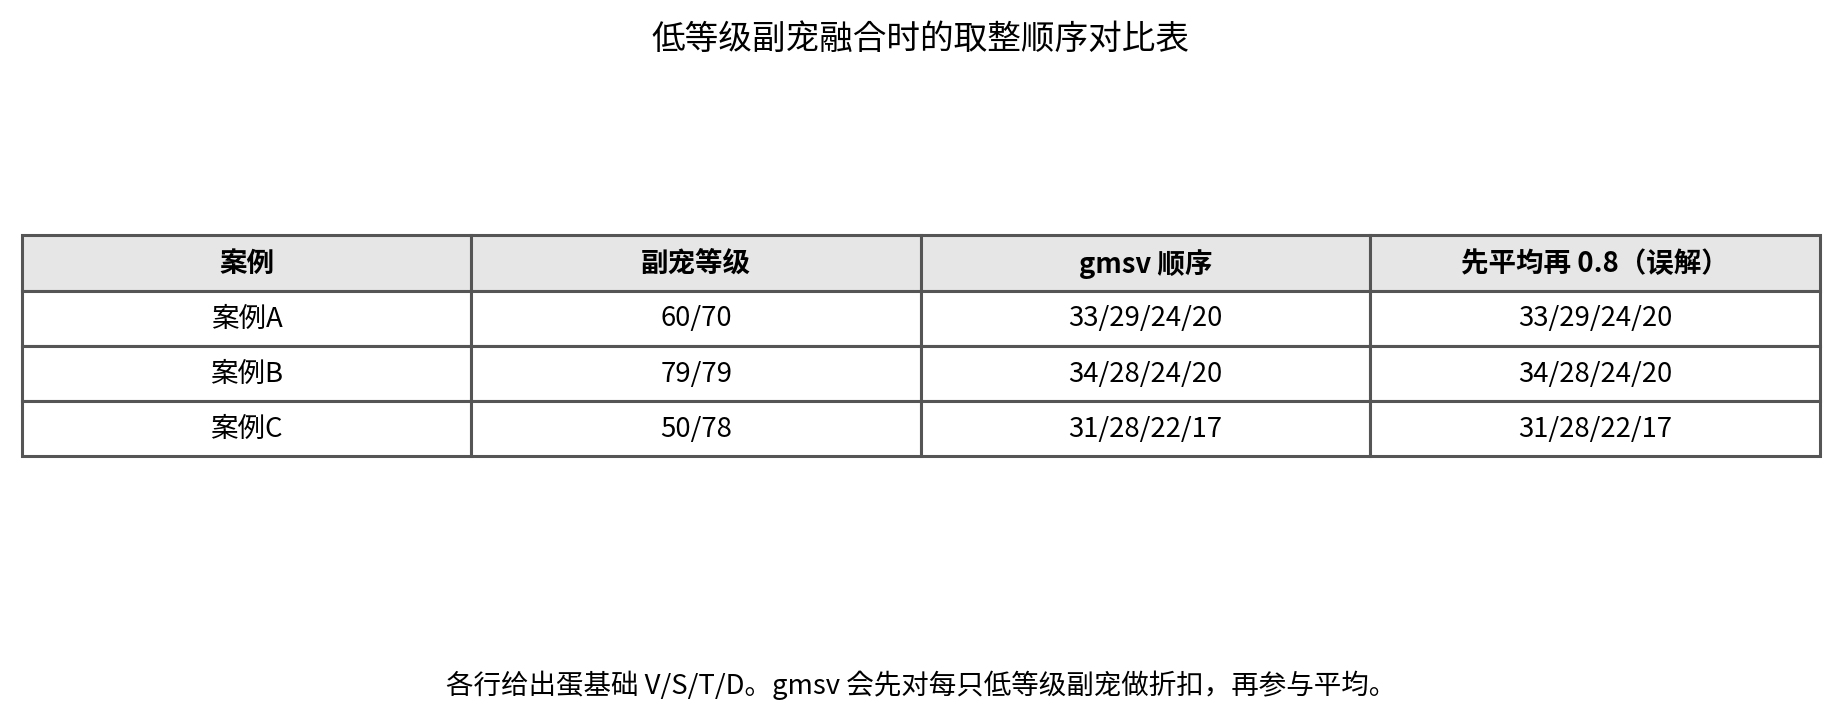
\includegraphics[width=0.86\textwidth]{figures/fusion_rounding_table.png}
    \caption{低等级副宠参与融合时的取整顺序对比。表中给出三组副宠案例，并比较 \code{gmsv} 实际采用的“各自先做 $0.8$ 折扣，再平均”与常见误解“先平均，再统一做 $0.8$ 折扣”所得到的蛋基础成长。可以看到，仅仅交换取整顺序就足以改变最终蛋面。}
    \label{fig:fusion-rounding-table}
\end{figure}

\section{蛋喂养模型}

\subsection{药效累加与折算}

蛋喂药的输入包括蛋基础成长 $\bm{b}$ 与一个 $4\times 5$ 的喂药方案矩阵。记第 $i$ 维在第 $\ell$ 级药上喂食的颗数为 $c_{i\ell}$，第 $\ell$ 级药的原始值为 $e_{\ell}$，则每一维的药效原始和为
\begin{equation}
    r_i = \sum_{\ell=1}^{5} c_{i\ell} e_{\ell}.
\end{equation}
在当前默认口径下，$e_{\ell}$ 依次为 $25,50,75,100,125$，且总喂食颗数固定为 $40$。原始药效不会直接加到成长档上，而是先折算为
\begin{equation}
    u_i = \min\left\{\left\lfloor \frac{7r_i}{1000} \right\rfloor,\,60\right\}.
    \label{eq:feed-fold}
\end{equation}
这一步对应“折算单项上限 $60$”。它说明高等级药和低等级药的效果虽然在线性原始值层面可相加，但一旦进入折算与上限，就会产生显著的离散差异。

\subsection{50 压缩与再分配}

记折算后的总和为
\begin{equation}
    U = \sum_{i=1}^{4} u_i.
\end{equation}
若 $U \le 50$，则直接令 $w_i=u_i$；若 $U>50$，则先做整体压缩：
\begin{equation}
    w_i = \left\lfloor \frac{50u_i}{U} \right\rfloor.
    \label{eq:work-cap}
\end{equation}
接下来，并不是把 $w_i$ 直接加到蛋基础成长上，而是再通过一轮“半折算 + 按比例回分配”生成孵化后成长。记
\begin{equation}
    T_1 = \sum_{i=1}^{4} w_i, \qquad T_2 = \sum_{i=1}^{4} b_i,
\end{equation}
并定义
\begin{equation}
    T = \left\lfloor \frac{T_1}{2} \right\rfloor + T_2.
\end{equation}
当前实现对每一维使用
\begin{equation}
    f_i = b_i + \left\lfloor \frac{w_i}{2} \right\rfloor,
\end{equation}
再计算增量
\begin{equation}
    \Delta_i = \left\lfloor \frac{f_i}{T} T_1 \right\rfloor,
\end{equation}
从而得到初步孵化成长
\begin{equation}
    h_i' = \operatorname{clip}_{[1,60]}\bigl(b_i + \Delta_i\bigr).
    \label{eq:hatch-pre}
\end{equation}
式~\eqref{eq:hatch-pre} 中最容易被忽略的细节是：系统使用的是 $w_i//2$ 和 $T_1//2$，而不是实数意义上的除以 $2$。因此，药效并入蛋成长时存在一层额外的整数损失，这也是喂药优化必须采用搜索而不是简单比例推算的原因之一。

\subsection{150 压缩与最终孵化成长}

记初步孵化成长总和为
\begin{equation}
    H' = \sum_{i=1}^{4} h_i'.
\end{equation}
若 $H' \le 150$，则最终孵化后成长直接取 $h_i=h_i'$；若 $H'>150$，则再施加一次总和压缩：
\begin{equation}
    h_i = \operatorname{clip}_{[1,60]}\left(\left\lfloor \frac{150h_i'}{H'} \right\rfloor\right).
    \label{eq:hatch-final}
\end{equation}
于是，当前工具中的“孵化后成长”本质上是由式~\eqref{eq:feed-fold}、式~\eqref{eq:work-cap}、式~\eqref{eq:hatch-pre} 和式~\eqref{eq:hatch-final} 共同决定的离散映射。它既不是药效与蛋成长的简单求和，也不是一个只需看总和的线性规划问题，而是同时受到单项上限、总和上限、比例回分配和多次向下取整约束的组合优化问题。

在默认参数 `40` 颗药、五级药原始值上限 `125` 的设定下，还有一个容易被忽略的事实：所有药的原始总和最多只有 $40 \times 125 = 5000$，因此折算后四维工作值总和满足
\begin{equation}
    \sum_i u_i \le \left\lfloor \frac{7 \times 5000}{1000} \right\rfloor = 35,
\end{equation}
从而式~\eqref{eq:work-cap} 中的 `50` 压缩在默认规则下实际上是休眠的。也就是说，当前默认喂药问题真正会起作用的总和约束，主要是后面的 `150` 孵化总和压缩，而不是前面的 `50` 工作值压缩。

\begin{figure}[H]
    \centering
    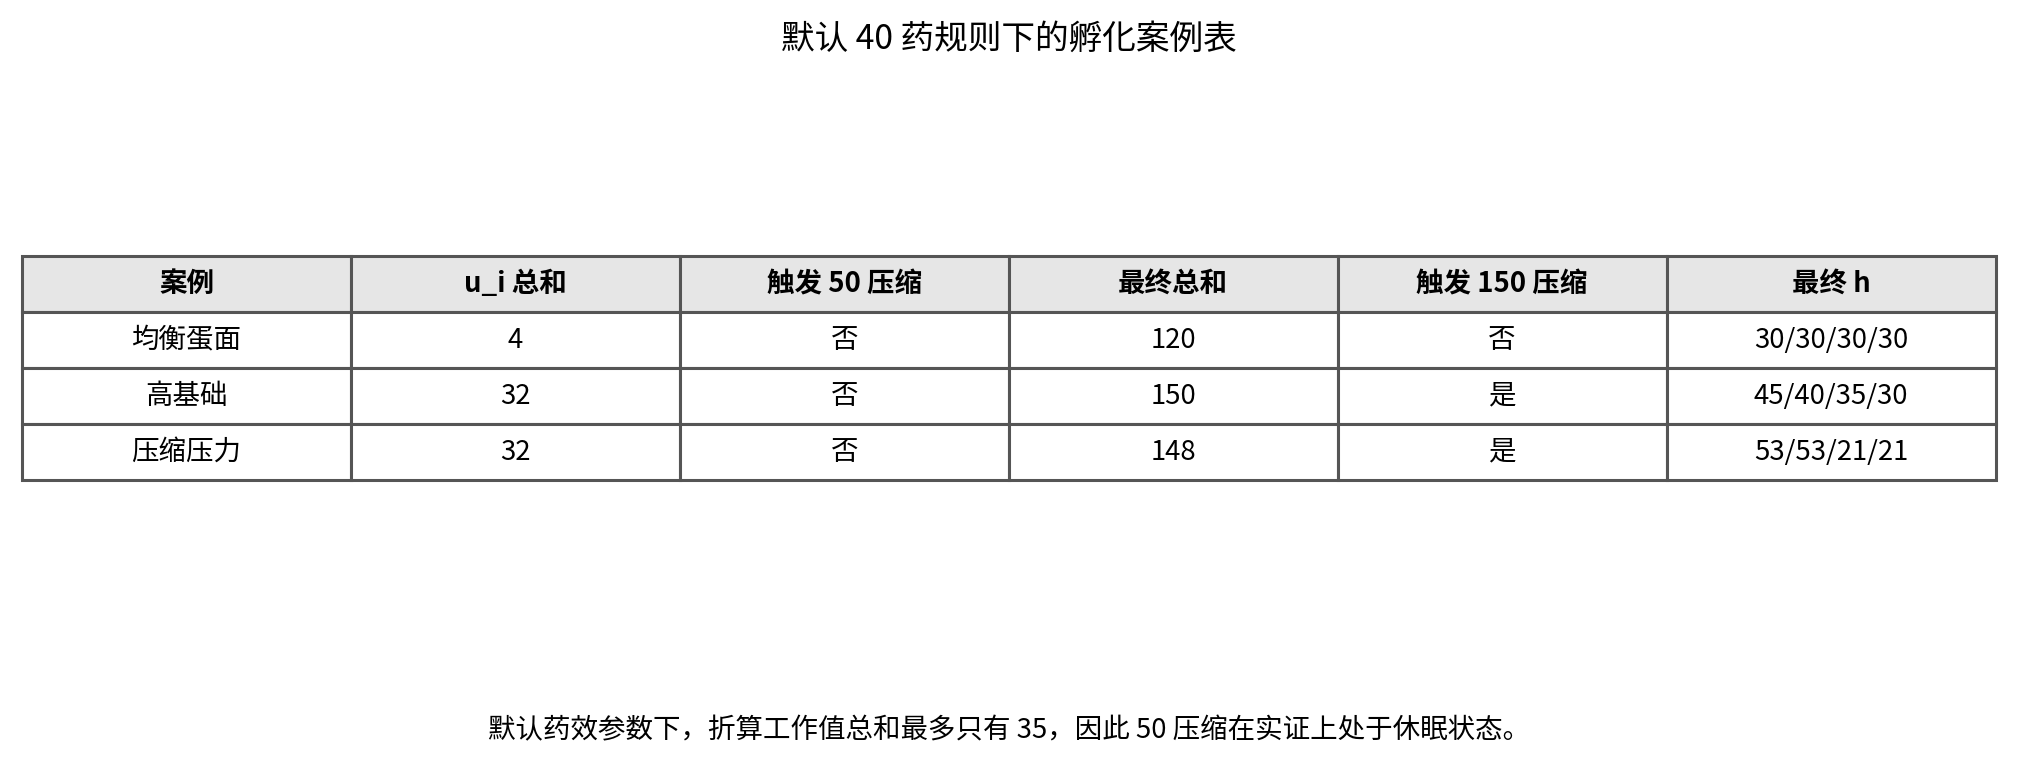
\includegraphics[width=0.9\textwidth]{figures/hatch_case_table.png}
    \caption{默认 `40` 药规则下的孵化案例表。表中列出不同蛋基础成长和喂药方案下的折算工作值总和、`50` 压缩是否触发、最终孵化总和以及 `150` 压缩是否触发。它直接展示了一个实证事实：在默认药效参数下，`50` 压缩不触发，而真正决定结果的常是最终 `150` 总和压缩。}
    \label{fig:hatch-case-table}
\end{figure}

若进一步把问题聚焦到“单项最终能否到 $60$”，则还会出现另一层阈值现象：即使某一维的喂药全部集中，只要其余三项总和过高，最终 `150` 压缩仍会把该维重新压回去。图~\ref{fig:hatch-threshold-table} 给出一个固定实验口径：把 `40` 颗五级药全部喂给敏捷维，并让其余三项基础成长尽量均分。表中列出的最小基础值阈值，正可以用来说明“为什么蛋面不到某个点，孵化后单项就上不去 $60$”。

\begin{figure}[H]
    \centering
    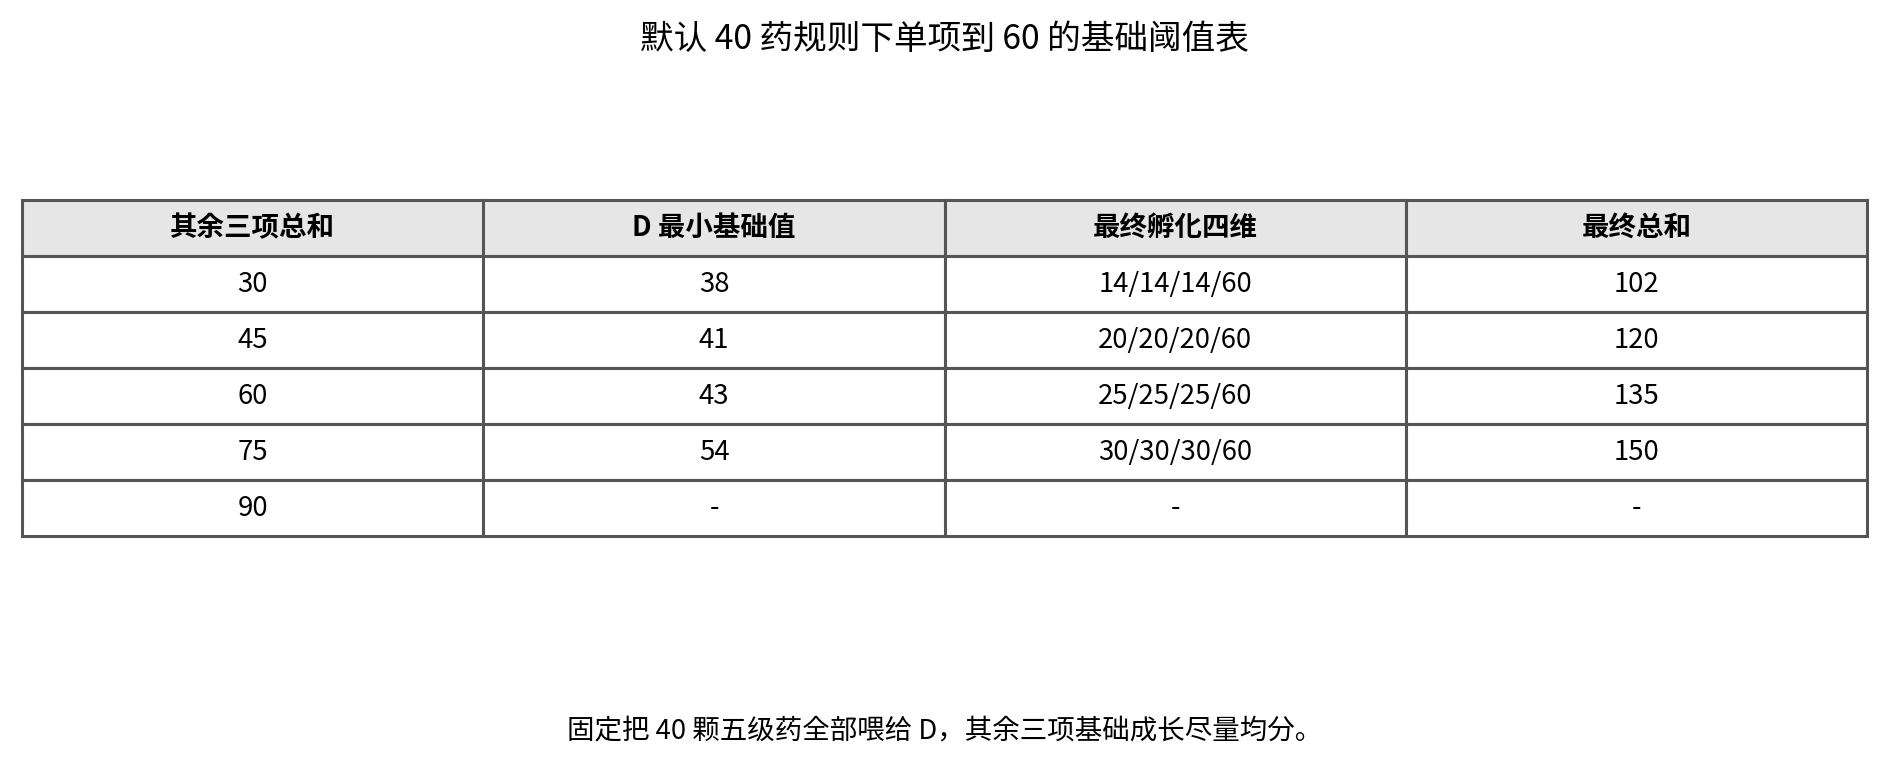
\includegraphics[width=0.84\textwidth]{figures/hatch_threshold_table.png}
    \caption{默认 `40` 药规则下单项到达 $60$ 的基础阈值表。固定把 `40` 颗五级药全部投入敏捷维，并令其余三项基础成长尽量均分，比较在不同“其余三项总和”下，敏捷维最终到达 $60$ 所需的最小蛋面基础值。}
    \label{fig:hatch-threshold-table}
\end{figure}

\section{孵化模型}

为了避免概念混乱，本文把“孵化”分成两个层次。第一层是当前工具所分析的\emph{确定性孵化成长}，也就是上一节得到的 $\bm{h}$；第二层是真正进入出生流程后的\emph{随机出生状态}，它还会叠加额外的随机扰动。对实际游戏过程而言，后者至少还可能包含四维独立的 $\pm2$ 波动、基于波动后总和的 Rank 判定，以及出生时的 $10$ 点随机加点。对当前论文和工具而言，主要优化对象是第一层，也就是不含出生后随机加点的孵化后成长。

这种分层处理有两个好处。第一，它把“喂药方案比较”与“出生运气比较”分开了：前者属于可控优化，后者属于随机结果。第二，它使得融合、喂药和普通成长之间的接口更加清晰。无论蛋来自哪种融合方案、喂了哪种药，最终都会先落到一个确定性的孵化成长向量 $\bm{h}$ 上，再由普通成长随机机制继续展开。

\section{养成链条的统一表示}

综合前述各节，本文将宠物养成系统写成如下统一流水线：
\begin{equation}
    \begin{aligned}
    \text{原宠} &\xrightarrow[]{\text{转生或保留}} \text{成长档} \xrightarrow[]{\text{融合}} \text{蛋基础成长 } \bm{b} \\
    &\xrightarrow[]{\text{喂药与孵化}} \text{孵化后成长 } \bm{h} \xrightarrow[]{\text{出生与升级随机}} \text{高等级面板}.
    \end{aligned}
\end{equation}
这条链的意义在于，它把原本散落在不同页面和不同源码函数中的机制统一成了一个状态变换序列。对工具开发而言，这意味着不同页面其实是在同一条链上截取不同节点；对后续战斗分析而言，这意味着命中、会心、先手和伤害所真正依赖的，不是某个孤立的喂药数值，而是整条养成流水线在终点处生成的有效成长与面板分布。

从研究角度看，本章最重要的结论不是某一条公式本身，而是所有这些公式共有的结构特征：它们几乎都不是连续线性过程，而是“先截断、再裁切、再按比例分配”的离散系统。也正因为如此，宠物培养问题天然适合被建模为离散优化与状态转移问题，而不是简单的线性加权问题。后文在讨论战斗表现与喂药最优方案时，将反复使用本章建立的这套离散流水线视角。

\chapter{战斗有效属性与状态变量}

若不先把战斗里真正参与判定的变量层次理清，后文关于乱敏、命中、会心、法术命中与属性状态的公式就很容易混成同一层。对当前 \code{gmsv} 而言，最重要的区别不是“面板属性和战斗属性谁更大”，而是“同一个中文词在源码里究竟落在哪个工作变量上”。本章因此先把人物、宠物、敌人在战斗中的有效属性层次、身份差异和常见状态变量整理出来。

\section{原始属性、固定属性与战斗属性}

从源码结构看，战斗中至少存在三层不同的属性口径。第一层是\emph{原始属性}，例如人物的 \code{CHAR_STR}、\code{CHAR_TOUGH}、\code{CHAR_DEX}、\code{CHAR_LUCK}，以及宠物由成长与等级生成后的显示攻击、防御、敏捷。它们更接近“回合开始前已经确定的基础值”。第二层是\emph{固定属性}，例如 \code{CHAR_WORKFIXSTR}、\code{CHAR_WORKFIXTOUGH}、\code{CHAR_WORKFIXDEX}、\code{CHAR_WORKFIXLUCK}，它们是在装备、套装、部分状态和战斗初始化结算之后写入的当前回合工作值。第三层则是\emph{战斗属性}，例如 \code{CHAR_WORKATTACKPOWER}、\code{CHAR_WORKDEFENCEPOWER}、\code{CHAR_WORKQUICK}，它们是在固定属性之上，再经过本回合的攻防速修正后得到的最终判定量。

把这一过程抽象写成函数链，可以记为
\begin{equation}
    X_{\mathrm{raw}}
    \xrightarrow{\;\mathcal{F}\;}
    X_{\mathrm{fix}}
    \xrightarrow{\;\mathcal{T}\;}
    X_{\mathrm{battle}},
\end{equation}
其中 $\mathcal{F}$ 表示装备、状态和战斗初始化引起的固定化过程，$\mathcal{T}$ 表示 \code{BATTLE_TurnParam()} 这一类“按本回合修正生成攻、防、速工作值”的过程。以敏捷为例，更具体的关系可以理解为
\begin{equation}
    \dex_{\mathrm{raw}} \longrightarrow \dex_{\mathrm{fix}}=\code{WORKFIXDEX}
    \longrightarrow Q=\code{WORKQUICK}.
\end{equation}
因此，玩家常说的“敏捷”在不同公式里并不总是指同一个量：行动顺序主要看 $Q$，而物理回避、会心、反击更多直接看 $\dex_{\mathrm{fix}}$。

幸运也存在类似分层，但其口径更容易混淆。物理回避、会心、反击常读的是固定幸运 \code{CHAR_WORKFIXLUCK}；而普通属性法术与职业法术命中，核心却仍直接读取原始幸运 \code{CHAR_LUCK}。这意味着“同样叫幸运”，在物理系统和法术系统里进入公式的位置并不一致。对玩家研究而言，这种变量层次差异比“某个系数是 $0.8$ 还是 $0.6$”更基础。

\section{人物、宠物与敌人的身份差异}

战斗公式中很多修正并不是由技能决定，而是先由单位身份决定。当前实现至少区分人物、宠物和敌方单位三类身份，它们会通过不同缩放系数进入同一条概率公式。以物理回避与会心为例，源码会根据“谁打谁”的组合，对攻方或守方敏捷先乘一次 $0.8$ 或 $0.6$ 再截断。其含义不是“宠物永远比较慢”或“人物永远更容易命中”，而是不同身份组合使用了不同的标准化口径。

从当前已核对的公式可抽象出两类最常见的身份差异。第一类是\emph{敏捷缩放差异}：人物打非人物、非人物打人物、敌人与宠物交战时，攻守双方敏捷会先做不同折扣，再进入回避或会心的平方根结构。第二类是\emph{替代变量差异}：当法术目标不是玩家时，系统往往不再读取幸运与抗魔装备，而改用目标等级作为近似项；当目标是宠物时，幸运在主 PVP 口径下通常也可近似视作 $0$。因此，“某技能打宠和打人感觉不一样”并不总来自技能本身，很多时候只是因为输入变量已经换了一套。

这种身份差异对后续章节有两个直接影响。其一，命中、回避、会心等热力图若只画“人物对人物”，不能直接外推到“人物对宠”或“宠对敌”；其二，宠物养成的价值不能只用人物 PVP 公式衡量，因为宠物本身落到战斗里时，输入层级和身份缩放都可能发生变化。也正因为此，后文在讨论“从宠物成长到战斗能力”时，会把人物、宠物、骑宠三种口径分开处理。

\section{常见战斗状态变量}

源码中的战斗状态并不都以“一个技能对应一个布尔量”的方式存在。更准确地说，它们是一组分散在 \code{CHAR_WORK*}、\code{CHAR_WORKBATTLEFLG}、\code{CHAR_WORKBATTLECOM*} 和战场全局结构中的状态槽。下面先列出对后文最关键的一组变量。

首先是若干会直接改变判定入口的布尔标记。防御动作 \code{BATTLE_COM_GUARD} 会让普通回避在最前面直接失败；\code{CHAR_BATTLEFLG_NODUCK} 表示“不能闪避”；\code{CHAR_BATTLEFLG_REVERSE} 则表示单位当前处于属性反转状态。其次是若干会改变具体参数的工作变量，例如 \code{CHAR_WORKBATTLECOM3} 会被当前动作复用，高 16 位和低 16 位在不同技能中可分别表示技能等级、子类型、阵列或额外修正值；\code{CHAR_MYSKILLHIT} 与 \code{CHAR_MYSKILLHIT_NUM} 则对应某些“提高命中”类主动状态。

这里还需要记住一个与宠物相关的战斗标记：\code{CHAR_BATTLEFLG_AIBAD}。本文把它称为宠物“\textbf{nono / 忠诚失控}”标记，它在 \code{BATTLE_PetLoyalCheck()} 中按回合清空后重新判断，表示该宠物这一回合没有按玩家原始指令行动；它会进一步影响反击、同队误伤保护等后续分支。

在回避系统里，还需要特别区分两套名字很像、但进入位置完全不同的状态。其一是 \code{_PETSKILL_SETDUCK} 相关的宠技回避状态，它主要借助 \code{CHAR_MYSKILLDUCK} 与 \code{CHAR_MYSKILLDUCKPOWER} 两个工作槽，分别记录剩余回合与独立前判概率；只要这层前判成功，整次物理攻击就直接判定为闪避。其二是职业技能 \textbf{回避} 对应的 \code{CHAR_WORK_P_DUCK} 与 \code{CHAR_WORKMOD_P_DUCK}，前者是“本回合是否启用该倍率”的标记，后者是倍率值；它们并不单独生成一次新的闪避事件，而是在普通回避值已经算出后再做乘法放大。

再往下是与属性系统直接相关的一组状态槽。四属性结界分别写在
\code{CHAR_WORKFIXEARTHAT_BOUNDARY}、
\code{CHAR_WORKFIXWATERAT_BOUNDARY}、
\code{CHAR_WORKFIXFIREAT_BOUNDARY}、
\code{CHAR_WORKFIXWINDAT_BOUNDARY}；
属性抗性会写入 \code{CHAR_WORK_F_RESIST}、\code{CHAR_WORK_I_RESIST}、\code{CHAR_WORK_T_RESIST}；场地属性、场地强度与回合数则存放在战场级结构 \code{BattleArray[battleindex]} 中。也就是说，属性系统并不是单一状态，而是一组作用层级不同、刷新逻辑也不同的子状态集合。

\section{状态变量的存储与回合更新}

从实现方式看，当前战斗状态大体可以分成三种。第一种是\emph{单纯标志位}，例如 \code{NODUCK}、\code{REVERSE} 等，通常通过按位与、按位或、按位异或来开关。第二种是\emph{整数槽位}，例如 \code{WORKFIXDEX}、\code{WORKQUICK}、各类抗性、各类命中附加，它们在每个回合的预处理阶段重新写入。第三种是\emph{高低位打包状态}，典型代表就是四属性结界使用的
\begin{equation}
    \code{MAKE2VALUE(power,turn)},
\end{equation}
它用高 16 位存强度、低 16 位存剩余回合。

状态的时间更新方式也并不统一。场地是战场级状态，每回合把 \code{att_count} 减一，减到非正时清空场地属性；四属性结界则是单位级状态，每回合把低 16 位回合数减一，减到 $-1$ 时清空该结界；属性反转则不是“每回合自动衰减”，而是靠技能再次命中时用异或切换开关。

从研究视角看，这些状态变量最重要的共性在于：它们不是平行地叠在最终伤害上，而是分散进入“预处理”“概率判定”“属性修正”“回合衰减”和“死亡收尾”等不同阶段。正因为状态进入位置不同，所谓“同样是减伤”或“同样是降敏”在源码里可能完全不是同一种机制。后续关于乱敏、法术命中、属性反转和骑宠伤害的章节，都会反复用到本章整理的变量层次与状态分类。


\chapter{行动顺序与乱敏机制}

行动顺序是石器时代战斗体验中最显性的结果之一，但它并不是一个“谁敏高谁先手”的静态比较，而是一个由参照敏捷、动作类型、骑宠混合和随机扰动共同决定的排序过程。本章的重点不是重复“乱敏存在”这一常识，而是把乱敏写成可分析的分段模型，并说明哪些技能真正吃骑宠混合敏，哪些技能其实只看人物自己的速度敏。

\section{普通行动的乱敏公式}

当前源码里，大多数普通行动都先取一个参照敏捷 $Q_{\mathrm{ref}}$，再把它写成
\begin{equation}
    w = Q_{\mathrm{ref}} + 20,
\end{equation}
最后生成顺序值
\begin{equation}
    S_{\mathrm{normal}} = w - \operatorname{RAND}(0,0.3w).
    \label{eq:turn-normal}
\end{equation}
式~\eqref{eq:turn-normal} 就是玩家口中的“乱敏”。它的含义不是“敏捷有一点随机误差”，而是顺序值会在区间
\begin{equation}
    S_{\mathrm{normal}} \in [0.7w,\; w]
\end{equation}
内波动。也就是说，敏捷优势并不会被完全抹平，但只要双方区间存在重叠，就仍有可能发生逆转。

道具使用与迅速类动作在这一基础上另有修正。道具顺序值可整理为
\begin{equation}
    S_{\mathrm{item}} = w - \operatorname{RAND}(0,0.3w) + 0.15w,
    \label{eq:turn-item}
\end{equation}
也就是在普通乱敏基础上再加 $15\%$。迅速攻击类则更激进，直接写成
\begin{equation}
    S_{\mathrm{quick}} = w + 0.3w = 1.3w,
    \label{eq:turn-quick}
\end{equation}
当前实现中这一段没有再附带随机扣减，因此它更像一个确定性的速度档提升，而不是“更高敏也照样大乱”的动作。

\section{道具、迅速行动与职业技能速度档}

从实现结构看，速度档并不只由“动作中文名”决定，而是由动作最终进入 \code{BATTLE_DexCalc()} 时走哪一条分支决定。最基础的一类是前节的默认档，即式~\eqref{eq:turn-normal}。第二类是物品档，即式~\eqref{eq:turn-item}。第三类是迅速档，即式~\eqref{eq:turn-quick}。除此以外，职业技能还会出现若干只看人物 \code{WORKQUICK} 的专用公式。

对于职业技能，最关键的区分是“该技能是否沿用默认档”。若沿用默认档，则其参照敏捷可能是人物敏，也可能是骑宠混合敏；若进入技能专用档，则公式常直接写作
\begin{equation}
    w = Q_c + 20,
\end{equation}
其中 $Q_c$ 是人物自己的 \code{WORKQUICK}，不再读取骑宠敏捷。于是，玩家常说的“骑宠会不会影响技能先手”，本质上不是职业问题，而是速度分支问题。

\section{三职业技能速度分类}

为避免把职业技能逐个列成源码表，本节采用“按速度分支分组”的方式整理三职业技能。这样做的好处是：一方面仍然保留源码口径，另一方面避免把研究重点淹没在冗长列表中。

\subsection{法师系}

法师系技能大多不走骑宠混合敏，而是直接以人物 \code{WORKQUICK} 为参照，再按不同随机范围扣减。令
\begin{equation}
    w_m = Q_c + 20.
\end{equation}
则常见分组如下：

\begin{table}[H]
    \centering
    \caption{法师系技能的主要速度档}
    \begin{tabularx}{\textwidth}{>{\raggedright\arraybackslash}p{4.2cm} >{\raggedright\arraybackslash}p{4.4cm} X}
        \toprule
        分组 & 速度公式 & 代表技能 \\
        \midrule
        快法术档 & $w_m-\operatorname{RAND}(0,0.2w_m)$ & 火山泉、召雷术、冰箭术 \\
        中速法术档 & $w_m-\operatorname{RAND}(0,0.3w_m)$ & 嗜血成性、嗜血蛊、一针见血 \\
        封印档 & $w_m-\operatorname{RAND}(0.3w_m,0.5w_m)$ & 火附体、冰附体、雷附体 \\
        重法术档 & $w_m-\operatorname{RAND}(0,0.5w_m)$ & 火星球、电流术、冰爆术 \\
        延迟重法档 & $w_m-\operatorname{RAND}(0.2w_m,0.5w_m)$ & 火龙枪、暴风雨、冰镜术、附身术、移形换位 \\
        \bottomrule
    \end{tabularx}
\end{table}

其中 \textbf{世界末日} 和 \textbf{火龙枪} 还带有延迟释放特性，因此“读到技能指令的回合”和“真正生效出手的回合”不是同一回合。对研究而言，这意味着法师的先手并不只是速度档问题，还与技能是否先进入延迟状态有关。

\subsection{白狼系}

白狼系主动战斗技能在当前分支下大多沿用默认档，因此速度公式仍可视为式~\eqref{eq:turn-normal}，区别只在于参照敏捷是否已经被骑宠混合。代表技能包括：爆击、连环攻击、回避、补血、双重攻击、激化攻击、专注战斗、盾击、格档、贯穿攻击、座骑攻击、濒死攻击、回旋攻击、混乱攻击等。

这组技能的共同特征是：若人物没有骑宠，则直接读人物速度敏；若人物处于骑宠状态，则其先手性质会明显受武器远近和骑宠敏捷影响。因此，白狼系的“速度构筑”不能脱离骑宠场景单独讨论。

\subsection{猎人系}

猎人系主动战斗技能同样大多走默认档，包括陷阱、驯伏宠物、激怒宠物、天罗地网、树根缠绕、体力掠夺、毒素武器、火抗性、冰抗性、雷抗性、自然威能、号召自然、四属性结界、团体三抗、弱点攻击、挑拨、遗忘等。和白狼系类似，它们的顺序值仍取决于默认档与骑宠混合敏，因此“猎人辅助技能会不会因为骑宠而变快”在当前实现下答案通常是肯定的。

\section{骑宠状态下的速度参照}

骑宠状态的关键不是“骑上后统一加一个速度值”，而是参照敏捷的来源会随远程武器和近战武器而变。设人物的战斗速度敏为 $Q_c=\code{WORKQUICK}$，骑宠的战斗速度敏为 $Q_p$。若某动作走默认档，则：

\begin{equation}
    Q_{\mathrm{ref}}=
    \begin{cases}
        Q_c, & \text{未骑宠},\\[4pt]
        0.8Q_c+0.2Q_p, & \text{骑宠且装备远程武器},\\[4pt]
        0.2Q_c+0.8Q_p, & \text{骑宠且装备近战武器或空手}.
    \end{cases}
    \label{eq:turn-ref-mounted}
\end{equation}

这里的“远程武器”并不只包括弓，还包括回力类和投掷类；源码里正是用 \code{BATTLE_IsThrowWepon()} 这一远程武器判定分支把它们归到同一类。式~\eqref{eq:turn-ref-mounted} 说明：骑宠远程本质上仍以人物为主，骑宠近战则明显转为宠物速度主导。也正因为此，同一只宠物在“给人物补近战先手”和“给人物补远程先手”两种用途下，敏捷价值并不相同。

若某技能走法师系那类专用速度档，则其参照敏捷通常退化为人物本体的 $Q_c$，而不使用式~\eqref{eq:turn-ref-mounted}。这就是为什么“骑宠对法师快法帮助有限”会在当前源码口径下成立。

\section{先手概率的变量分析}

把乱敏写成区间模型后，很多先手结论可以直接用支持区间判断。设双方行动都走默认档，分别对应
\begin{equation}
    w_a = Q_{\mathrm{ref},a}+20,\qquad w_b = Q_{\mathrm{ref},b}+20.
\end{equation}
则它们的顺序值支撑区间分别为
\begin{equation}
    S_a \in [0.7w_a,w_a], \qquad S_b \in [0.7w_b,w_b].
\end{equation}
于是可以立刻得到三类结论：
\begin{equation}
    0.7w_a > w_b \;\Longrightarrow\; a \text{ 必定先手},
\end{equation}
\begin{equation}
    w_a < 0.7w_b \;\Longrightarrow\; a \text{ 不可能先手},
\end{equation}
其余情况则属于区间重叠区，需要做离散随机比较。

这一结果的意义非常直接。第一，先手不是“敏捷高一点就更稳”，而是只有当最小顺序值已经压过对方最大顺序值时，才会进入确定先手区。第二，提升速度的收益具有阶段性：在远离阈值时，边际收益体感很弱；一旦接近 $0.7$ 与 $1.0$ 形成的边界，少量敏捷就可能明显改变先手概率。第三，骑宠近战和骑宠远程由于改变了 $Q_{\mathrm{ref}}$ 的来源，实际上会把整条先手阈值曲线一起平移。

从更一般的研究角度看，精确先手概率需要处理离散随机变量
\begin{equation}
    S = w - \operatorname{RAND}(0,\rho w)
\end{equation}
的卷积比较，其中 $\rho$ 取 $0.2,0.3,0.5$ 等不同档位。当前项目更适合把这一问题交给枚举或模拟，而不是强行写成封闭初等函数；但就变量影响分析而言，前述区间判据已经足以解释绝大多数实战中的“为什么这套配置经常被反超”或“为什么某个骑宠一换武器先手就变了”的现象。

\begin{figure}[H]
    \centering
    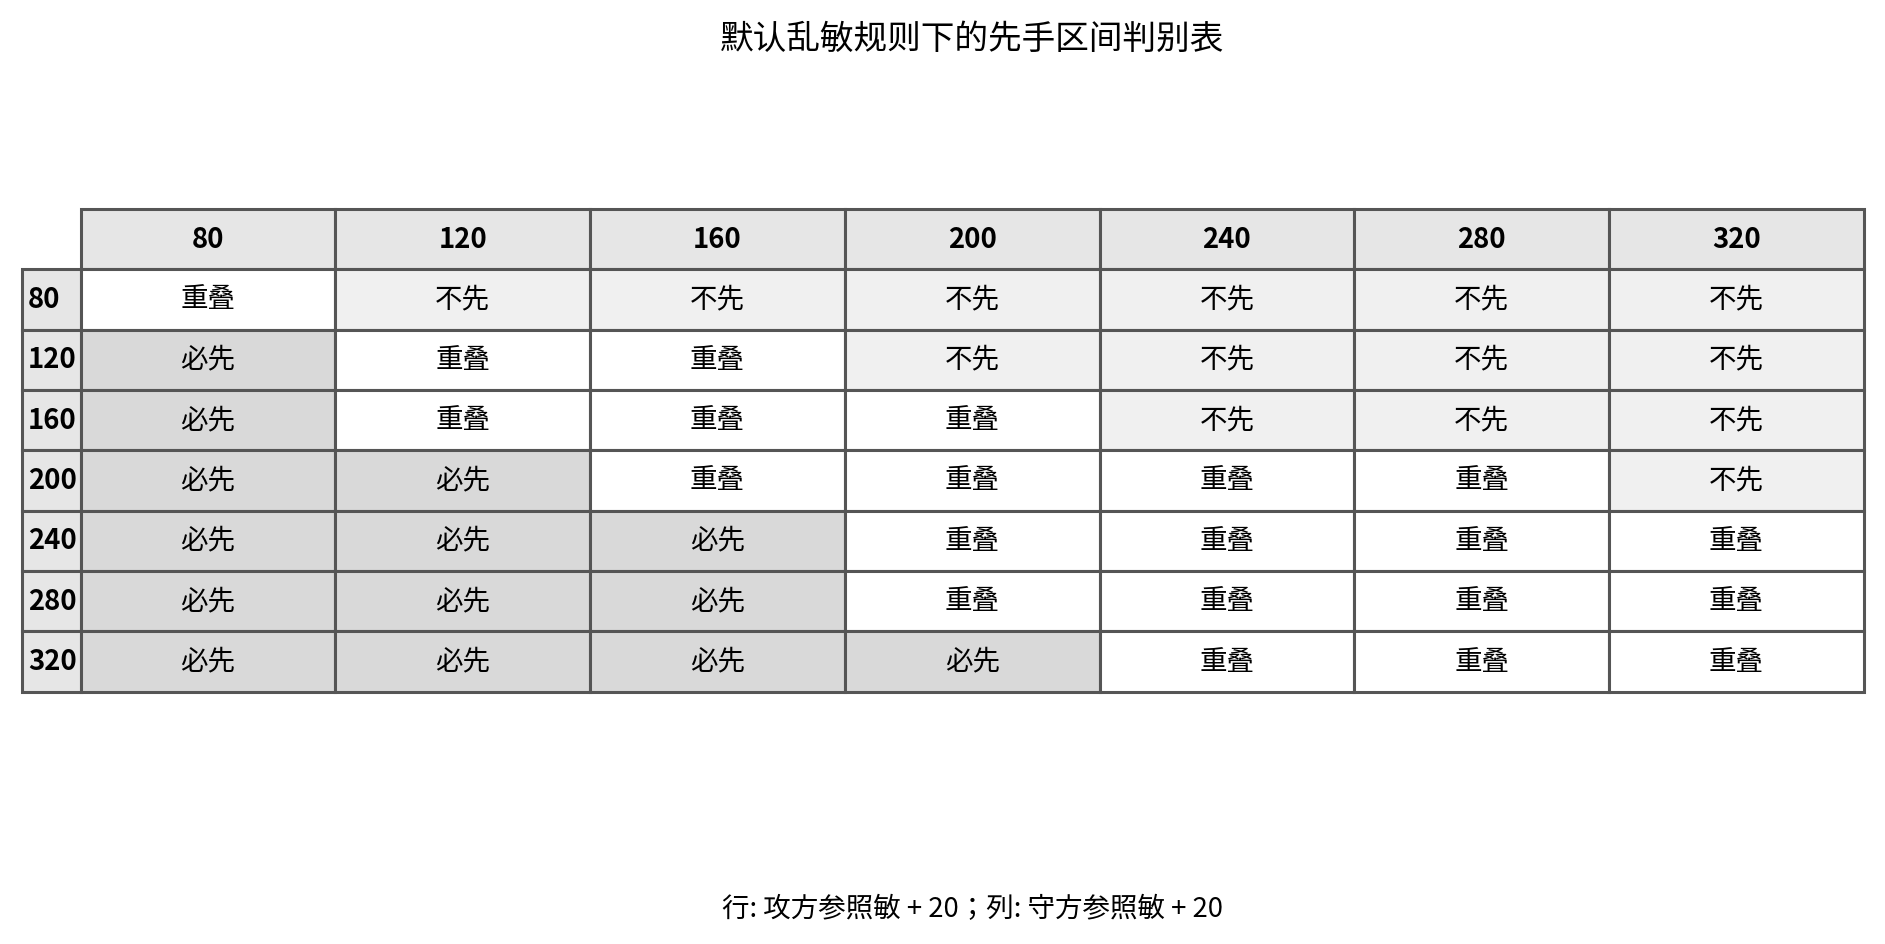
\includegraphics[width=0.88\textwidth]{figures/turn_region_table.png}
    \caption{默认乱敏规则下的先手区间判别表。图中以 $w_a=Q_{\mathrm{ref},a}+20$、$w_b=Q_{\mathrm{ref},b}+20$ 为行列，\texttt{Always} 表示攻方必定先手，\texttt{Never} 表示攻方不可能先手，\texttt{Overlap} 表示双方顺序值区间重叠，需进一步做离散随机比较。}
    \label{fig:turn-region-table}
\end{figure}


\chapter{物理命中、回避、会心与反击}

\section{普通回避的源码判定顺序}

源码中物理攻击的判定顺序为：先检查防守方是否具备\emph{根本不能闪}的条件,再进入普通回避主体。”回避率”分为三层：硬性失败条件、独立前判、普通回避公式本身。

普通回避的硬性失败条件包括：当前动作是 \code{BATTLE\_COM\_GUARD}\footnote{\code{gmsv/src/battle/battle.c}, 第2847行。}、存在吸收/反射/消失类伤害反应、当前无法行动且不满足”集气但未被天罗地网或盾击限制”的例外、挂有 \code{CHAR\_BATTLEFLG\_NODUCK}，以及特殊战斗标记。这些条件一旦命中,后续不再进入普通回避公式。

若编译启用 \code{_PETSKILL\_SETDUCK}\footnote{\code{gmsv/src/include/version.h}, 第287行。},防守方可能在普通回避前先经过额外回避前判。该前判读取 \code{CHAR\_MYSKILLDUCK} (剩余回合) 与 \code{CHAR\_MYSKILLDUCKPOWER} (前判成功率)。

\begin{theorem}[回避前判与普通回避的复合]
\label{thm:duck-front-composite}
设前判成功率为 $p_{\mathrm{front}}$,普通回避主体成功率为 $p_{\mathrm{normal}}$,则总闪避率为
\begin{equation}
    p_{\mathrm{total}} = p_{\mathrm{front}} + \bigl(1-p_{\mathrm{front}}\bigr)p_{\mathrm{normal}}.
\end{equation}
\end{theorem}

\begin{proof}
前判失败概率为 $1-p_{\mathrm{front}}$,此时进入普通回避,成功率为 $p_{\mathrm{normal}}$。两阶段独立,总成功率为前判成功加前判失败后普通回避成功。
\end{proof}

\begin{remark}
职业技能 \textbf{回避} 不是独立前判。\code{CHAR\_WORK\_P\_DUCK} 仅为”启用倍率”标记,\code{CHAR\_WORKMOD\_P\_DUCK} 为倍率值；两者将已算出的普通回避值乘以比例,属于普通回避主体的后段修正。
\end{remark}

\section{命中与回避的源码公式}

\subsection{身份修正与主判定顺序}

设攻击方与防守方原始固定敏分别为 $\attdex$ 与 $\defdex$。进入普通回避主体前,源码按攻守身份做\emph{单边修正}\footnote{\code{gmsv/src/battle/battle.c}, 第2865-2890行。},而非对两边同时缩放。记修正后的固定敏为 $\widetilde{\attdex}$ 与 $\widetilde{\defdex}$,则在当前主分支下可整理为
\begin{equation}
    (\widetilde{\attdex},\widetilde{\defdex})=
    \begin{cases}
        (\lfloor 0.8\attdex \rfloor,\defdex), & \text{敌人打宠物}, \\
        (\attdex,\lfloor 0.8\defdex \rfloor), & \text{非敌人打宠物}, \\
        (\lfloor 0.6\attdex \rfloor,\defdex), & \text{非玩家打玩家}, \\
        (\attdex,\lfloor 0.6\defdex \rfloor), & \text{玩家打非玩家}, \\
        (\attdex,\defdex), & \text{其余情形}.
    \end{cases}
\end{equation}
所有取整来自源码将浮点乘法结果回写到整型变量的截断。

令
\begin{equation}
    B = \max\{\widetilde{\attdex},\widetilde{\defdex}\}, \qquad S = \min\{\widetilde{\attdex},\widetilde{\defdex}\},
\end{equation}
并定义比例项
\begin{equation}
    w = \begin{cases}
        1, & \widetilde{\defdex} \ge \widetilde{\attdex}, \\
        \dfrac{\widetilde{\defdex}}{\widetilde{\attdex}}, & \widetilde{\defdex} < \widetilde{\attdex}.
    \end{cases}
\end{equation}
再定义动作参数
\begin{equation}
    \alpha = \begin{cases}
        0.027, & \text{若防守方当前动作是 \code{BATTLE\_COM\_JYUJYUTU}（咒术）}, \\
        0.02, & \text{否则}.
    \end{cases}
\end{equation}
则普通回避主体的核心基础值为
\begin{equation}
    d_{\mathrm{core}} = \sqrt{\max\!\left\{\frac{B-S}{\alpha},0\right\}}\,w.
\end{equation}

在此之后，源码按如下顺序继续叠加或修正：
\begin{equation}
    d_{\mathrm{pre}} = d_{\mathrm{core}} + L_d + M + R_{\mathrm{drunk}} + 40I_{\mathrm{bow}} + N,
\end{equation}
\begin{equation}
    u_0 = \operatorname{clip}_{[1,7500]}\!\bigl(100d_{\mathrm{pre}}\bigr),
\end{equation}
\begin{equation}
    u_1 = \max\{0, u_0 - R_{\mathrm{hit}}\},
\end{equation}
\begin{equation}
    u_2 = \left\lfloor \frac{u_1(100+P)}{100} \right\rfloor,
\end{equation}
\begin{equation}
    u_3 = \begin{cases}
        1.4u_2, & \text{若攻击方当前使用混乱攻击}, \\
        u_2, & \text{否则}.
    \end{cases}
\end{equation}
最终以 \code{RAND(1,10000) <= u3}\footnote{\code{gmsv/src/battle/battle.c}, 第2923行。} 判定是否闪避成功。这里 $L_d$ 表示防守方幸运；$M$ 表示全局回避修正 \code{gBattleDuckModyfy}；$R_{\mathrm{drunk}}$ 表示攻击方醉酒时附加的 \code{RAND(20,30)}，否则取 $0$；$I_{\mathrm{bow}}$ 为攻击方是否持弓的指示量，源码该分支额外加两次 $20$；$N$ 表示 \code{BATTLE\_COM\_S\_NOGUARD} 带来的技能附加值；$R_{\mathrm{hit}}$ 表示 \code{AddHit} 在后段扣掉的命中修正；$P$ 表示职业技能 \textbf{回避} 的倍率加成。


\subsection{咒术动作分支与职业技能是否共用回避链}

从源码命名与分支用途看,\code{BATTLE\_COM\_JYUJYUTU}\footnote{\code{gmsv/src/include/battle.h}, 第45行。} 译作”\textbf{咒术动作分支}”。该常量名对应日文”咒术”的罗马字写法；现代常见拼写为 \emph{jujutsu},源码保留较旧的 \code{JYUJYUTU} 形式。式~\eqref{eq:dodge-base} 中 $\alpha=0.027$ 的触发条件仅看\emph{防守方当前动作}是否为 \code{BATTLE\_COM\_JYUJYUTU},不看攻击方是否使用职业技能。

职业技能下达动作时统一写入各自的 \code{BATTLE\_COM\_S\_*},不直接标记为 \code{BATTLE\_COM\_JYUJYUTU}。”使用职业技能”与”进入咒术回避参数分支”不是同一件事。需要区分的是：该职业技能后续是否仍调用普通物理攻击序列 \code{BATTLE\_AttackSeq()}\footnote{\code{gmsv/src/battle/battle.c}, 第1847行。},从而继续进入 \code{BATTLE\_DuckCheck()}\footnote{\code{gmsv/src/battle/battle.c}, 第2847行。}。若是,则仍受”目标当前动作是 \code{BATTLE\_COM\_JYUJYUTU}”影响；若否,则不按本章的普通物理回避链解释。表~\ref{tab:profession-dodge-paths} 汇总当前源码下的关键分类。

\begin{table}[H]
    \centering
    \caption{职业技能与普通物理回避链的关系}
    \label{tab:profession-dodge-paths}
    \begin{tabularx}{\textwidth}{>{\raggedright\arraybackslash}p{2.7cm} >{\raggedright\arraybackslash}p{3.8cm} >{\raggedright\arraybackslash}p{3.8cm} >{\centering\arraybackslash}p{1.8cm} X}
        \toprule
        技能类别 & 代表技能 & 主要结算入口 & 调用 \code{BATTLE\_DuckCheck} & 是否受目标 \code{JYUJYUTU} 的 $0.027$ 影响 \\
        \midrule
        直接物理职业攻击 & 爆裂、连环攻击、双重攻击、骑宠攻击、舍命攻击、弱点攻击、掠夺、混乱攻击 & \code{battle\_profession\_attack\_fun()} $\rightarrow$ \code{BATTLE\_AttackSeq()} & 是 & 是；但触发前提仍是\emph{目标当前动作}为 \code{BATTLE\_COM\_JYUJYUTU} \\
        带物理命中判定的状态攻击 & 盾击、剧毒武器 & \code{battle\_profession\_status\_chang\_fun()} $\rightarrow$ \code{BATTLE\_AttackSeq()} & 是 & 是；逻辑与直接物理职业攻击相同 \\
        辅助与自我强化技能 & 专注战斗、回避、回复、舍己为人、激怒、能量聚集、陷阱、驯化等 & \code{battle\_profession\_assist\_fun()} & 否 & 否；不按普通物理回避链处理 \\
        法师攻击技能 & 火球、冰箭、火枪、雷击、末日、血蛊等 & \code{battle\_profession\_attack\_magic\_fun()} $\rightarrow$ \code{PROFESSION\_MAGIC\_ATTAIC()} & 否 & 否；应按职业法术命中链分析 \\
        主分发归入法术攻击组的特殊技能 & 穿透攻击、缠绕攻击 & 当前主分发进入职业法术攻击组 & 本文暂不按普通物理回避链归类 & 本文暂不把它们并入 $\alpha=0.027$ 的普通物理回避分析，留待后续校核 \\
        \bottomrule
    \end{tabularx}
\end{table}

表~\ref{tab:profession-dodge-paths} 的含义可压缩为：\textbf{职业技能不因”职业技能”身份自动进入 \code{BATTLE\_COM\_JYUJYUTU} 分支；仅那些后续仍调用普通物理回避函数的职业技能,才会在目标当前动作恰好是咒术分支时,间接受到 $\alpha=0.027$ 的影响。}

\subsection{PVP 内部的人宠对象组合差异}

即使在玩家对玩家战斗中,\emph{人打人、人打宠、宠打人、宠打宠} 也不能共用同一简化公式。源码先按攻击侧与防守侧的单位类型进入不同分支,再决定缩放哪一边的固定敏,以及是否切到线性口径。表~\ref{tab:pvp-pairings} 汇总当前源码下三类物理概率机制在 PVP 内部的对象组合差异。这里”人”指玩家本体,”宠”指玩家宠物。

\begin{table}[H]
    \centering
    \caption{PVP 中不同攻守对象组合的概率口径差异}
    \label{tab:pvp-pairings}
    \begin{tabularx}{\textwidth}{>{\raggedright\arraybackslash}p{1.8cm} X X X X}
        \toprule
        机制 & 人打人 & 人打宠 & 宠打人 & 宠打宠 \\
        \midrule
        回避 & 无身份缩放；守方幸运生效 & 守方敏先截断为 $\lfloor 0.8\defdex \rfloor$ & 攻方敏先截断为 $\lfloor 0.6\attdex \rfloor$；守方幸运生效 & 守方敏先截断为 $\lfloor 0.8\defdex \rfloor$ \\
        会心 & $\beta=0.09$，平方根口径；攻方幸运与武器会心生效 & 守方敏先截断为 $\lfloor 0.6\defdex \rfloor$；其余同人打人 & 改为 $\beta=10$ 的线性口径；通常无幸运项、无武器会心项 & $\beta=0.09$，平方根口径；通常无幸运项、无武器会心项 \\
        反击 & $\gamma=0.08$，平方根口径；武器矩阵 $F$ 与幸运生效 & 守方敏先截断为 $\lfloor 0.6\defdex \rfloor$；仍读武器矩阵 $F$ 与幸运 & 改为 $\gamma=10$ 的线性口径；走宠物反击分支，不读武器矩阵 $F$ 与幸运，\code{NOGUARD} 可加值 & $\gamma=0.08$，平方根口径；走宠物反击分支，不读武器矩阵 $F$ 与幸运，\code{NOGUARD} 可加值 \\
        \bottomrule
    \end{tabularx}
\end{table}

其中有两个易错点。第一,回避判断中”人打宠”与”宠打宠”都命中”防守方是宠物”分支,因此都将守方固定敏截断到 $0.8$ 倍,而非常被误写的 $0.6$ 倍。第二,会心与反击的身份分支不完全等于回避：当攻击侧是宠物、防守侧是玩家时,两者都切到”除以 10 且不开根号”的线性口径。

后文给出显式导数和切片图时,统一固定在”人打人”支路上；人打宠、宠打人和宠打宠需按表~\ref{tab:pvp-pairings} 先切换到对应口径,再进入各自的离散计算。

\subsection{玩家打玩家的离散化简式}

若只考虑玩家对玩家,并忽略额外前判、弓、醉酒、\code{AddHit}、职业技能 \textbf{回避}、无防御攻击附加与混乱攻击修正,则有 $\widetilde{\attdex}=\attdex$、$\widetilde{\defdex}=\defdex$。

\begin{definition}[普通回避基础体]
\label{def:dodge-base}
在玩家 PVP 简化条件下,普通回避基础体定义为
\begin{equation}
    d_{\mathrm{base}}(\attdex,\defdex)=
    \begin{cases}
        \sqrt{\dfrac{\defdex-\attdex}{0.02}}, & \defdex \ge \attdex, \\
        \sqrt{\dfrac{\attdex-\defdex}{0.02}}\dfrac{\defdex}{\attdex}, & \defdex < \attdex.
    \end{cases}
    \label{eq:dodge-base}
\end{equation}
\end{definition}

\begin{theorem}[离散化普通回避率]
\label{thm:duck-discrete}
在玩家 PVP 简化口径下,源码对应的普通回避率为离散化结果:
\begin{equation}
    p_{\mathrm{duck}}^{\mathrm{src}}(\attdex,\defdex,L)
    = 0.01\min\!\left\{7500,\max\!\left\{1,\left\lfloor 100\bigl(d_{\mathrm{base}}(\attdex,\defdex)+L\bigr)\right\rfloor\right\}\right\}.
    \label{eq:dodge-final}
\end{equation}
普通命中率为
\begin{equation}
    p_{\mathrm{hit}}^{\mathrm{src}}(\attdex,\defdex,L)=100.00-p_{\mathrm{duck}}^{\mathrm{src}}(\attdex,\defdex,L).
    \label{eq:hit-final}
\end{equation}
\end{theorem}

\begin{remark}
式~\eqref{eq:dodge-final} 与式~\eqref{eq:hit-final} 是当前源码在玩家 PVP 简化条件下的离散百分比结果；后文做导数分析时,暂时去掉取整与上下限裁切,只保留对应的连续化主体。图~\ref{fig:dodge-heatmap} 展示回避率在攻守敏捷平面上的分布,图~\ref{fig:hit-slice} 展示命中率随攻方敏捷的变化。
\end{remark}

\begin{figure}[H]
\centering
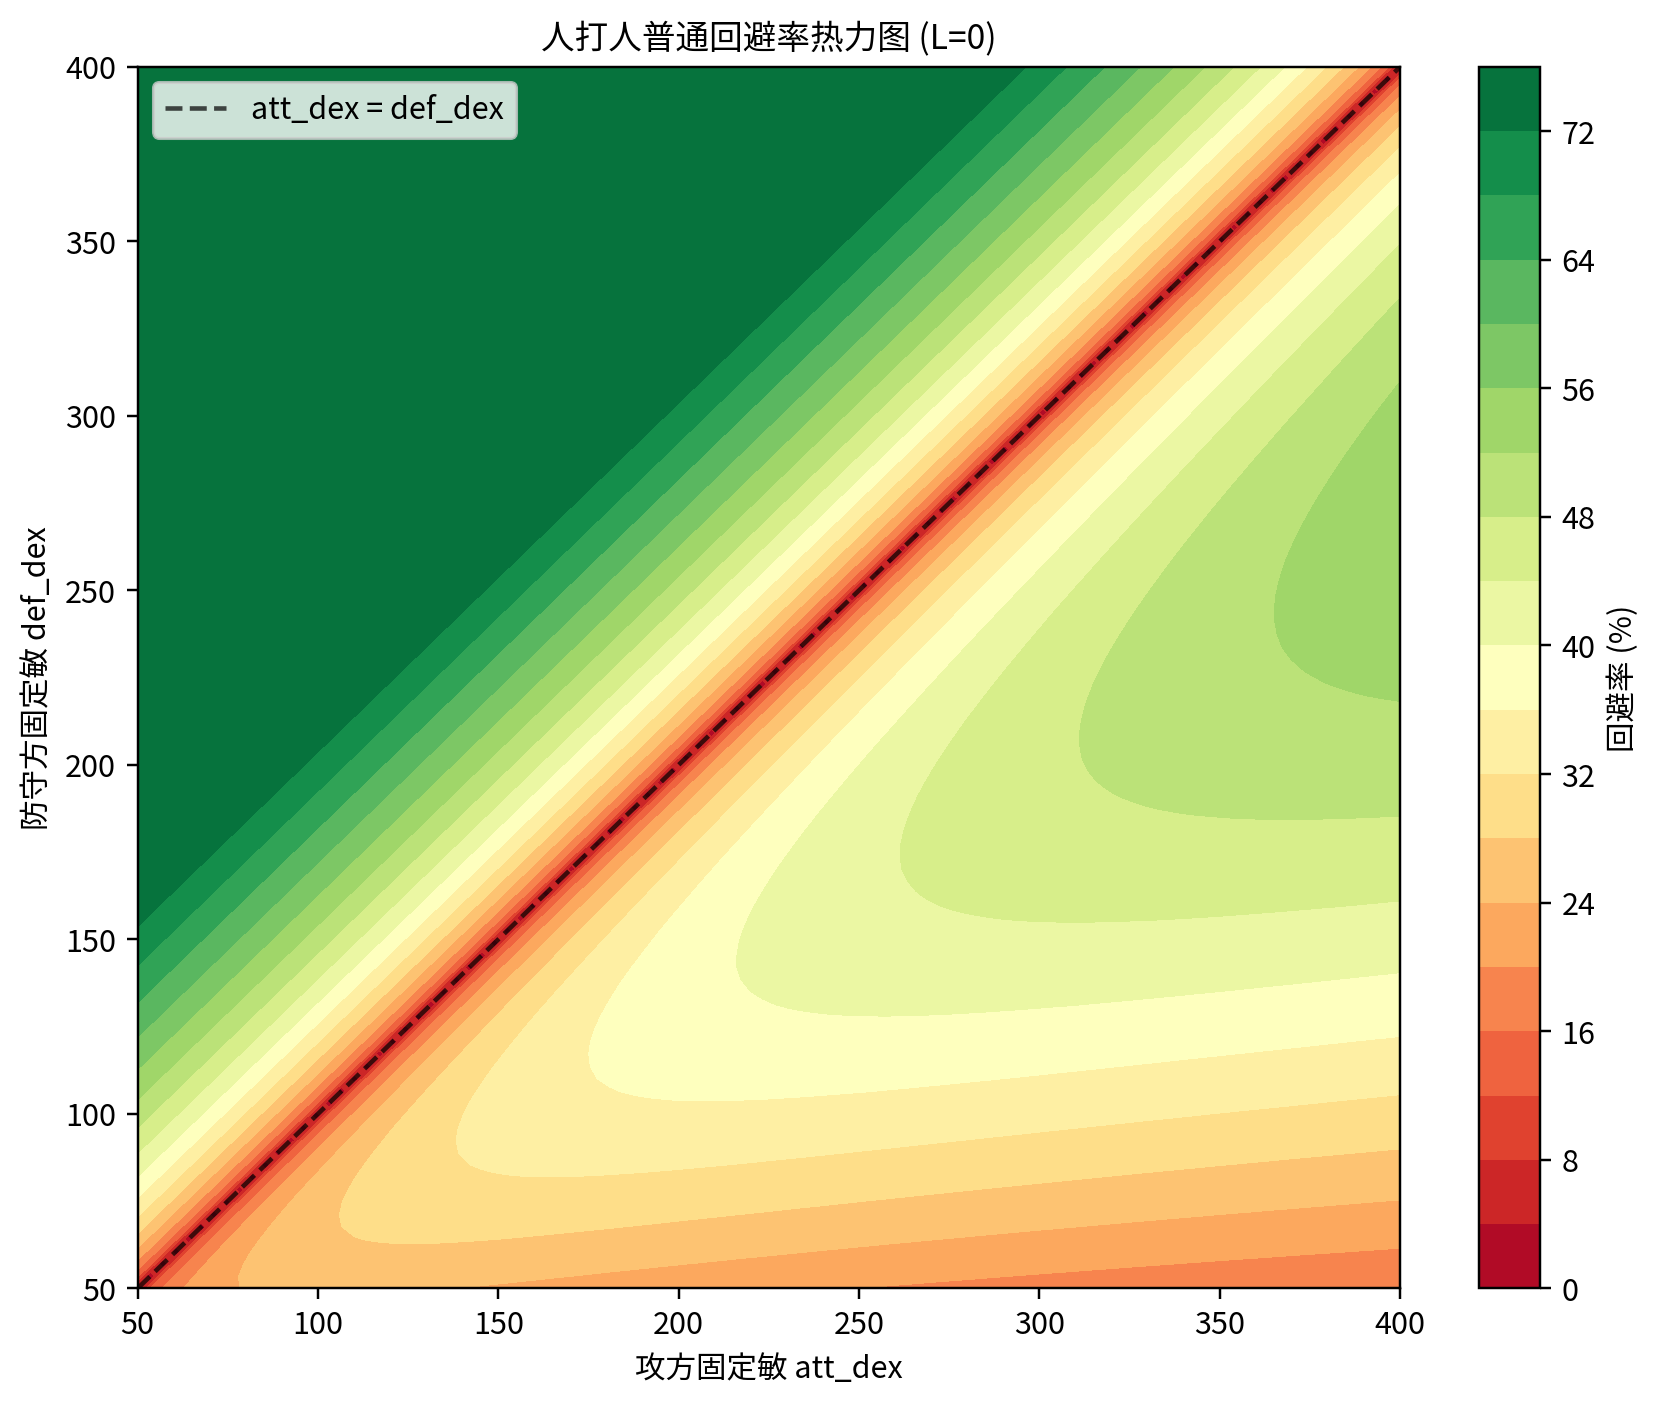
\includegraphics[width=0.75\textwidth]{figures/dodge_heatmap.png}
\caption{人打人普通回避率热力图 ($L=0$)}
\label{fig:dodge-heatmap}
\end{figure}

\begin{figure}[H]
\centering
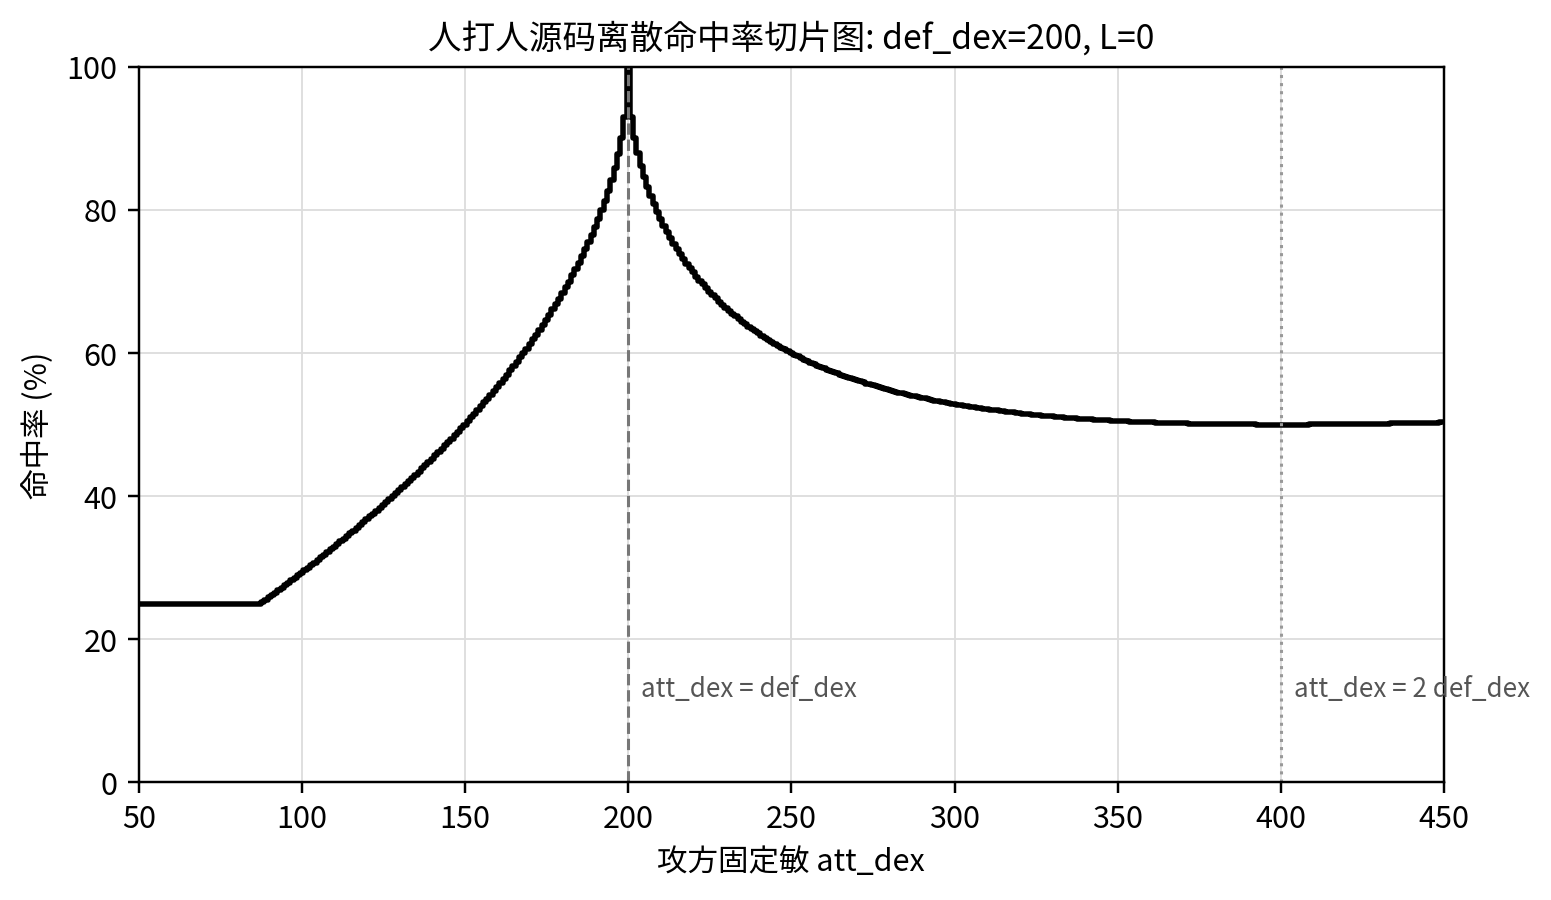
\includegraphics[width=0.75\textwidth]{figures/hit_slice_y200.png}
\caption{人打人命中率切片图 ($\defdex=200, L=0$)}
\label{fig:hit-slice}
\end{figure}

\subsection{实战上最容易写错的细节}

这一段源码里有四个非常容易被简化过头的细节。其一，身份修正不是“攻守两边都按同一规则缩放”，而是按对象组合只修一边。其二，弓修正会在普通回避流程中加两次。其三，\code{AddHit} 发生在 $[1,7500]$ 裁切之后，而职业技能 \textbf{回避} 的倍率又发生在 \code{AddHit} 之后。其四，混乱攻击会在这些步骤之后再把当前回避值提高 $40\%$。这几个步骤的相对顺序不能交换，否则就会得到与源码不同的边界结果。

\section{会心公式与武器会心}

\subsection{源码顺序与身份修正}

会心判定与回避不同，并不共享同一套身份修正规则。设攻击方与防守方原始固定敏仍为 $\attdex$ 与 $\defdex$，武器会心值为 $C$，攻击方幸运为 $L_a$。在当前主分支下，会心公式的身份修正可整理为
\begin{equation}
    (\widehat{\attdex},\widehat{\defdex},\beta,\rho)=
    \begin{cases}
        (\attdex,\lfloor 0.8\defdex \rfloor,0.09,\sqrt{\cdot}), & \text{宠物打敌人}, \\
        (\attdex,\defdex,10,\mathrm{id}), & \text{敌人打宠物}, \\
        (\attdex,\defdex,10,\mathrm{id}), & \text{非玩家打玩家}, \\
        (\attdex,\lfloor 0.6\defdex \rfloor,0.09,\sqrt{\cdot}), & \text{玩家打非玩家}, \\
        (\attdex,\defdex,0.09,\sqrt{\cdot}), & \text{其余情形}.
    \end{cases}
\end{equation}
其中 $\rho$ 记号用来区分“平方根口径”和“线性口径”：若 $\rho=\sqrt{\cdot}$，源码取平方根；若 $\rho=\mathrm{id}$，则直接取一次差值，不再开根。

令
\begin{equation}
    B = \max\{\widehat{\attdex},\widehat{\defdex}\}, \qquad S = \min\{\widehat{\attdex},\widehat{\defdex}\},
\end{equation}
并定义
\begin{equation}
    w = \begin{cases}
        1, & \widehat{\attdex} \ge \widehat{\defdex}, \\
        \dfrac{\widehat{\attdex}}{\widehat{\defdex}}, & \widehat{\attdex} < \widehat{\defdex}.
    \end{cases}
\end{equation}
则会心基础体为
\begin{equation}
    c_{\mathrm{core}} =
    \begin{cases}
        \sqrt{\max\!\left\{\dfrac{B-S}{\beta},0\right\}} + 0.5C, & \rho=\sqrt{\cdot}, \\
        \max\!\left\{\dfrac{B-S}{\beta},0\right\} + 0.5C, & \rho=\mathrm{id},
    \end{cases}
\end{equation}
\begin{equation}
    c_{\mathrm{raw}} = c_{\mathrm{core}}\,w + L_a.
\end{equation}
源码随后执行
\begin{equation}
    c_{\mathrm{work}} = \min\!\left\{10000,\max\!\left\{1,\left\lfloor 100c_{\mathrm{raw}}\right\rfloor\right\}\right\},
\end{equation}
并以 \code{RAND(1,10000) < c\_work} 判定是否会心成立。

\subsection{玩家打玩家的离散化简式}

对玩家 PVP 而言，上述身份修正退化为 $\widehat{\attdex}=\attdex$、$\widehat{\defdex}=\defdex$、$\beta=0.09$ 且采用平方根口径，于是连续基础体可写为
\begin{equation}
    c_{\mathrm{base}}(\attdex,\defdex,L,C)=
    \begin{cases}
        \sqrt{\dfrac{\attdex-\defdex}{0.09}}+L+0.5C, & \attdex \ge \defdex, \\
        \left(\sqrt{\dfrac{\defdex-\attdex}{0.09}}+0.5C\right)\dfrac{\attdex}{\defdex}+L, & \attdex < \defdex.
    \end{cases}
    \label{eq:crit-base}
\end{equation}
对应的源码离散化会心率为
\begin{equation}
    p_{\mathrm{crit}}^{\mathrm{src}}(\attdex,\defdex,L,C)
    = 0.01\min\!\left\{9999,\max\!\left\{0,\left\lfloor 100c_{\mathrm{base}}(\attdex,\defdex,L,C)\right\rfloor-1\right\}\right\}.
    \label{eq:crit-final}
\end{equation}
之所以是减去 $1$，是因为源码最终使用的是严格小于号 \code{<}，而不是回避公式中的小于等于号 \code{<=}。

另一个非常容易被误解的点是弓。当前实现中，弓并非“不能会心”，而是“即使判出会心，也不走额外的会心伤害函数”。换言之，弓在概率意义上仍可产生会心事件，但该事件在伤害层面的收益会被显著削弱。

\section{反击触发条件、离散公式与次数上限}

\subsection{触发条件}

反击并不是一个无条件概率，而是一系列条件之后的后验事件。首先，当前出手动作必须属于可反击类型，当前主分支主要对应普通攻击与无防御攻击。其次，反击方和被反击方都必须存活。再次，带有本回合忠诚失控标记 \code{CHAR_BATTLEFLG_AIBAD} 的单位不能触发反击。最后，若任意一边使用的是弓、回力或投掷类远程武器，反击检查会直接失败。

源码主循环还显式限制了反击链的最大往返次数，因此反击不是无限触发过程，而是一个带有深度上限的离散链式事件。

\subsection{玩家打玩家时的反击离散化简式}

设反击方与被反击方固定敏分别为 $\attdex$ 与 $\defdex$。反击基础敏捷体与会心类似，但不带武器会心项。对玩家 PVP 简化口径，有
\begin{equation}
    q_{\mathrm{base}}(\attdex,\defdex)=
    \begin{cases}
        \sqrt{\dfrac{\attdex-\defdex}{0.08}}, & \attdex \ge \defdex, \\
        \sqrt{\dfrac{\defdex-\attdex}{0.08}}\dfrac{\attdex}{\defdex}, & \attdex < \defdex.
    \end{cases}
    \label{eq:counter-base}
\end{equation}
记武器对武器系数为 $F$，反击方幸运为 $L$。若忽略 \code{_SUIT\_ADDENDUM} 下的额外反击修正，则源码中的玩家反击工作值可写成
\begin{equation}
    r_{\mathrm{counter}} = 0.1F\,q_{\mathrm{base}}(\attdex,\defdex)+L.
\end{equation}
最终的源码离散化反击率为
\begin{equation}
    p_{\mathrm{counter}}^{\mathrm{src}}(\attdex,\defdex,L,F)
    = 0.01\min\!\left\{10000,\max\!\left\{0,\left\lceil 100r_{\mathrm{counter}}\right\rceil-1\right\}\right\}.
    \label{eq:counter-final}
\end{equation}
这里之所以出现上取整与减去 $1$，正是因为源码最终比较的是 \code{RAND(1,10000) < 100*r\_counter}。若讨论宠物反击，则还要额外加入 \code{BATTLE\_COM\_S\_NOGUARD} 的附加值，并注意宠物分支会在进入随机判定前显式裁切到 $100\%$。

\section{变量影响分析与单调性讨论}

以下讨论只针对“人打人”这条玩家 PVP 支路的\emph{连续化主体}，即暂时忽略回避、会心、反击公式中的取整、上下限裁切，以及严格小于或小于等于带来的 $0.01\%$ 级偏移。这样做的目的不是替代源码，而是把源码离散结果背后的主导趋势提取出来。

\subsection{命中对攻方敏捷并非全局单调}

先把式~\eqref{eq:dodge-final} 与式~\eqref{eq:hit-final} 中的取整与裁切去掉，只保留连续主体。此时命中率对攻方敏捷的导数满足：当 $\attdex<\defdex$ 时，
\begin{equation}
    \frac{\partial p_{\mathrm{hit}}}{\partial \attdex} = \frac{1}{2\sqrt{0.02}\sqrt{\defdex-\attdex}} > 0,
\end{equation}
因此攻方敏捷低于守方时，继续补敏一定提高命中。然而当 $\attdex>\defdex$ 时，
\begin{equation}
    \frac{\partial p_{\mathrm{hit}}}{\partial \attdex}
    = \frac{\defdex(\attdex-2\defdex)}{2\sqrt{0.02}\,\attdex^2\sqrt{\attdex-\defdex}}.
    \label{eq:hit-derivative}
\end{equation}
式~\eqref{eq:hit-derivative} 的符号取决于 $\attdex-2\defdex$，于是会出现三个区间：$\defdex<\attdex<2\defdex$ 时导数为负，$\attdex=2\defdex$ 时导数为零，$\attdex>2\defdex$ 时导数重新转正。也就是说，在“刚刚超过守方敏捷但还没到两倍”的区间里，继续堆攻方敏捷反而可能降低命中率。

\subsection{会心存在局部非单调区间}

对式~\eqref{eq:crit-base} 的连续主体，若先固定 $L$ 与 $C$，当 $\attdex>\defdex$ 时有
\begin{equation}
    \frac{\partial p_{\mathrm{crit}}}{\partial \attdex} = \frac{1}{2\sqrt{0.09}\sqrt{\attdex-\defdex}} > 0,
\end{equation}
因此攻方敏捷领先后，会心率单调上升。然而在 $\attdex<\defdex$ 且先忽略武器会心时，
\begin{equation}
    \frac{\partial p_{\mathrm{crit}}}{\partial \attdex} = \frac{2\defdex-3\attdex}{2\defdex\sqrt{0.09}\sqrt{\defdex-\attdex}}.
    \label{eq:crit-derivative}
\end{equation}
由式~\eqref{eq:crit-derivative} 可知，当 $\attdex<2\defdex/3$ 时，会心率随攻方敏捷增加而上升；当 $2\defdex/3<\attdex<\defdex$ 时，会心率反而下降。武器会心 $C$ 的存在会把这一拐点向右推移，但不能消除非单调结构本身。

\subsection{反击的主导单调性与会心同型}

对式~\eqref{eq:counter-final}，若暂时去掉上取整与边界裁切，只保留连续主体 $0.1F\,q_{\mathrm{base}}+L$，则当 $\attdex>\defdex$ 时有
\begin{equation}
    \frac{\partial p_{\mathrm{counter}}}{\partial \attdex}
    = \frac{F}{20\sqrt{0.08}\sqrt{\attdex-\defdex}} > 0.
\end{equation}
而在 $\attdex<\defdex$ 时，
\begin{equation}
    \frac{\partial p_{\mathrm{counter}}}{\partial \attdex}
    = \frac{F(2\defdex-3\attdex)}{20\defdex\sqrt{0.08}\sqrt{\defdex-\attdex}}.
    \label{eq:counter-derivative}
\end{equation}
因此，对固定正武器系数 $F$ 而言，反击在单调性上与“武器会心取 $0$ 的会心公式”完全同型：当 $\attdex<2\defdex/3$ 时先升，进入 $2\defdex/3<\attdex<\defdex$ 后转为下降，越过 $\attdex=\defdex$ 后重新单调上升。武器系数 $F$ 的作用主要是对整条曲线做比例缩放，而不是改变拐点位置。

\subsection{变量位置不同，收益性质就不同}

综合回避、会心与反击三条链可以看到：幸运、武器会心、武器对武器系数、\code{AddHit}、职业技能 \textbf{回避} 与混乱攻击修正，并不是在同一层进入公式。幸运大多表现为平移项；武器会心只作用于会心；武器对武器系数只作用于玩家反击；\code{AddHit} 发生在回避上限裁切之后；职业技能 \textbf{回避} 则发生在 \code{AddHit} 之后再做倍率放大。也正因为如此，石器时代里“每加一点某属性的收益”并不是统一线性的概念，而必须放回变量真正进入判定链的位置来讨论。

\section{源码离散值表与切片图}

图~\ref{fig:hit-crit-table} 与图~\ref{fig:hit-crit-slices} 都只画“人打人”这条支路。具体地，固定守方敏捷为 $\defdex=200$，并统一取守方幸运 $L_d=0$、攻方幸运 $L_a=0$、武器会心值 $C=0$、玩家反击武器系数 $F=10$，同时忽略弓、醉酒、\code{AddHit}、职业技能 \textbf{回避}、无防御攻击附加与混乱攻击修正。表中给出的命中率、会心率与反击率，均按本章的源码离散化简式直接计算，而不是用连续近似值代替。

\begin{figure}[H]
    \centering
    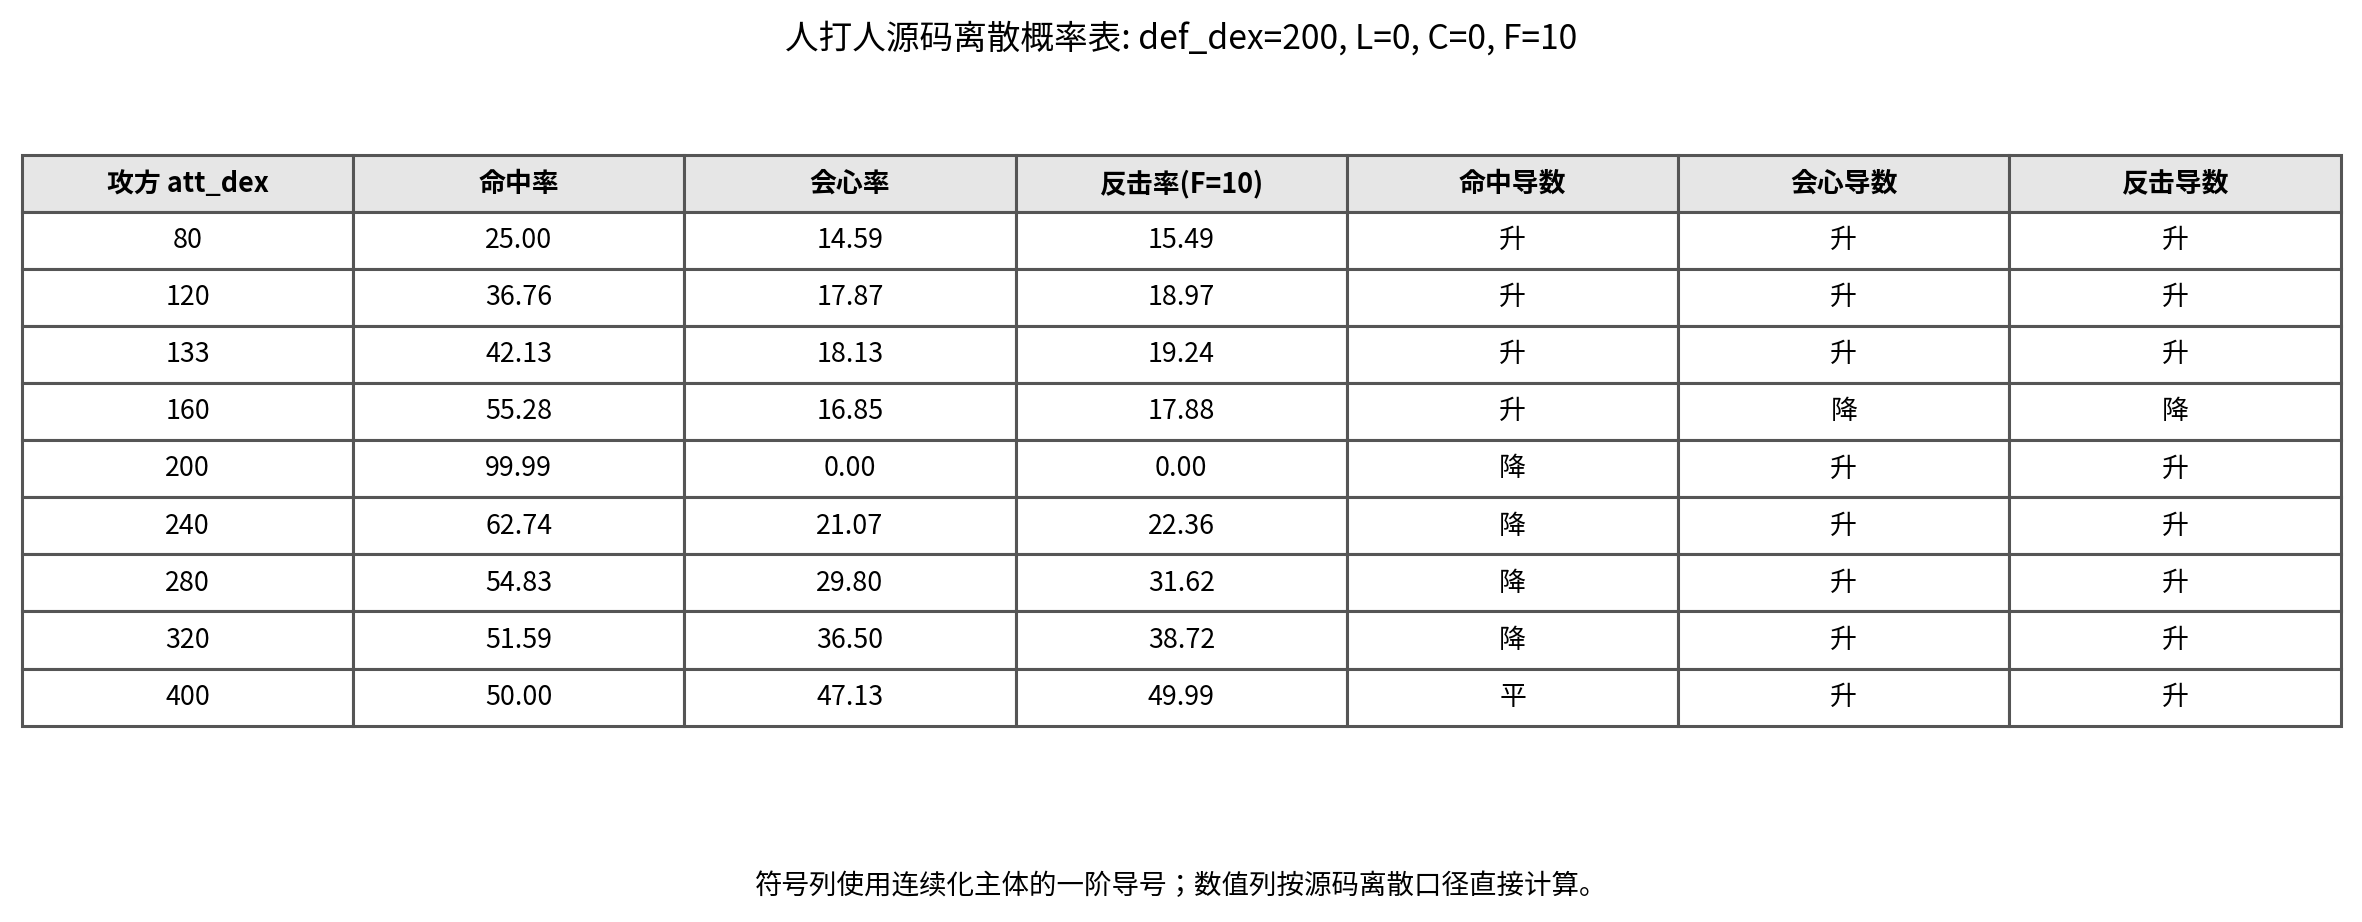
\includegraphics[width=0.9\textwidth]{figures/hit_crit_table_y200.png}
    \caption{固定守方敏捷 $\defdex=200$ 时的源码离散概率表。统一取 $L_d=L_a=0$、$C=0$、$F=10$，并关闭弓、醉酒、\code{AddHit}、职业技能 \textbf{回避}、无防御攻击附加与混乱攻击修正。表中符号列使用连续化主体的一阶导号，只用于展示主导趋势。}
    \label{fig:hit-crit-table}
\end{figure}

图~\ref{fig:hit-crit-slices} 进一步给出同一组参数下的切片图。三张图中的曲线都来自源码离散化简式，因此会呈现出台阶状；而虚线和点线标记的则是连续化主体中的关键阈值，用于说明“源码离散结果”和“连续趋势分析”之间是如何对应的。

\begin{figure}[H]
    \centering
    \begin{subfigure}[b]{0.48\textwidth}
        \centering
        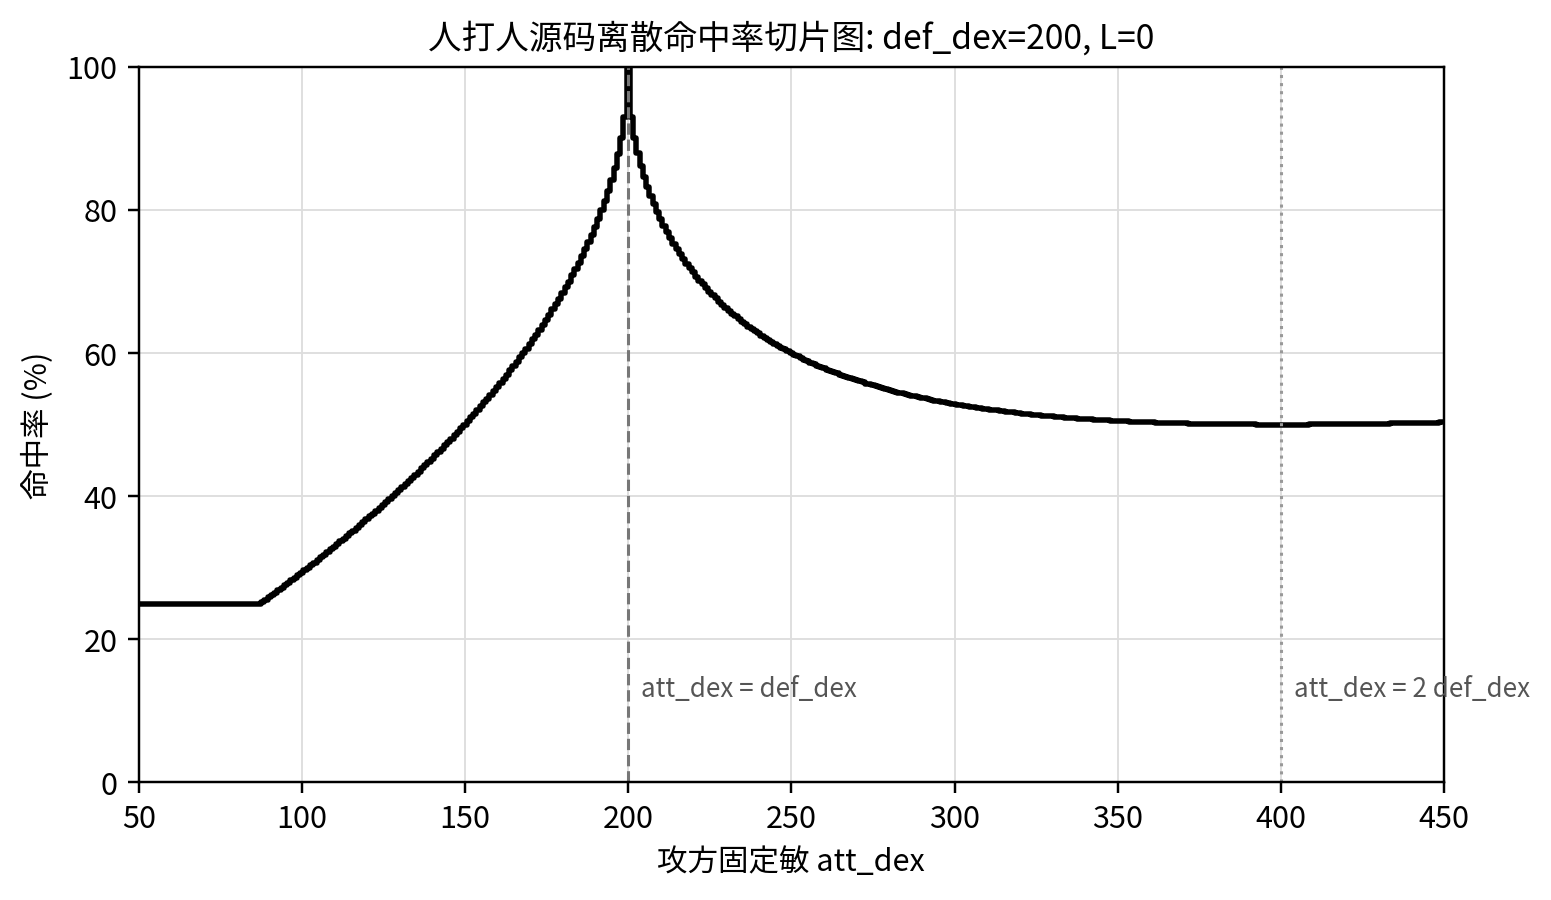
\includegraphics[width=\textwidth]{figures/hit_slice_y200.png}
        \caption{命中率切片图}
    \end{subfigure}
    \hfill
    \begin{subfigure}[b]{0.48\textwidth}
        \centering
        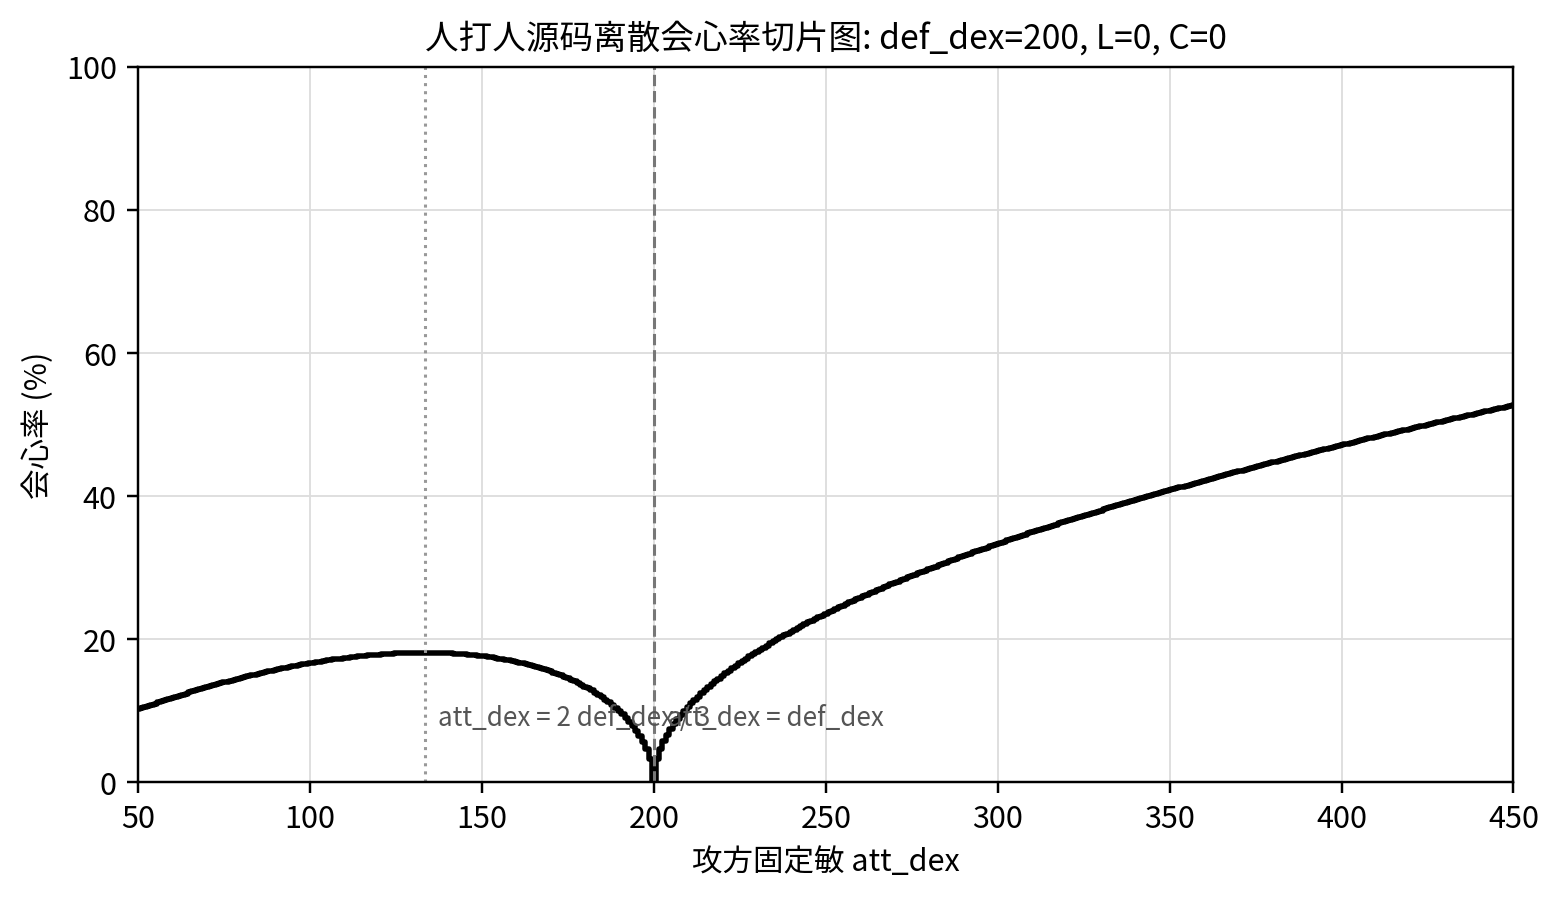
\includegraphics[width=\textwidth]{figures/crit_slice_y200.png}
        \caption{会心率切片图}
    \end{subfigure}

    \medskip
    \begin{subfigure}[b]{0.66\textwidth}
        \centering
        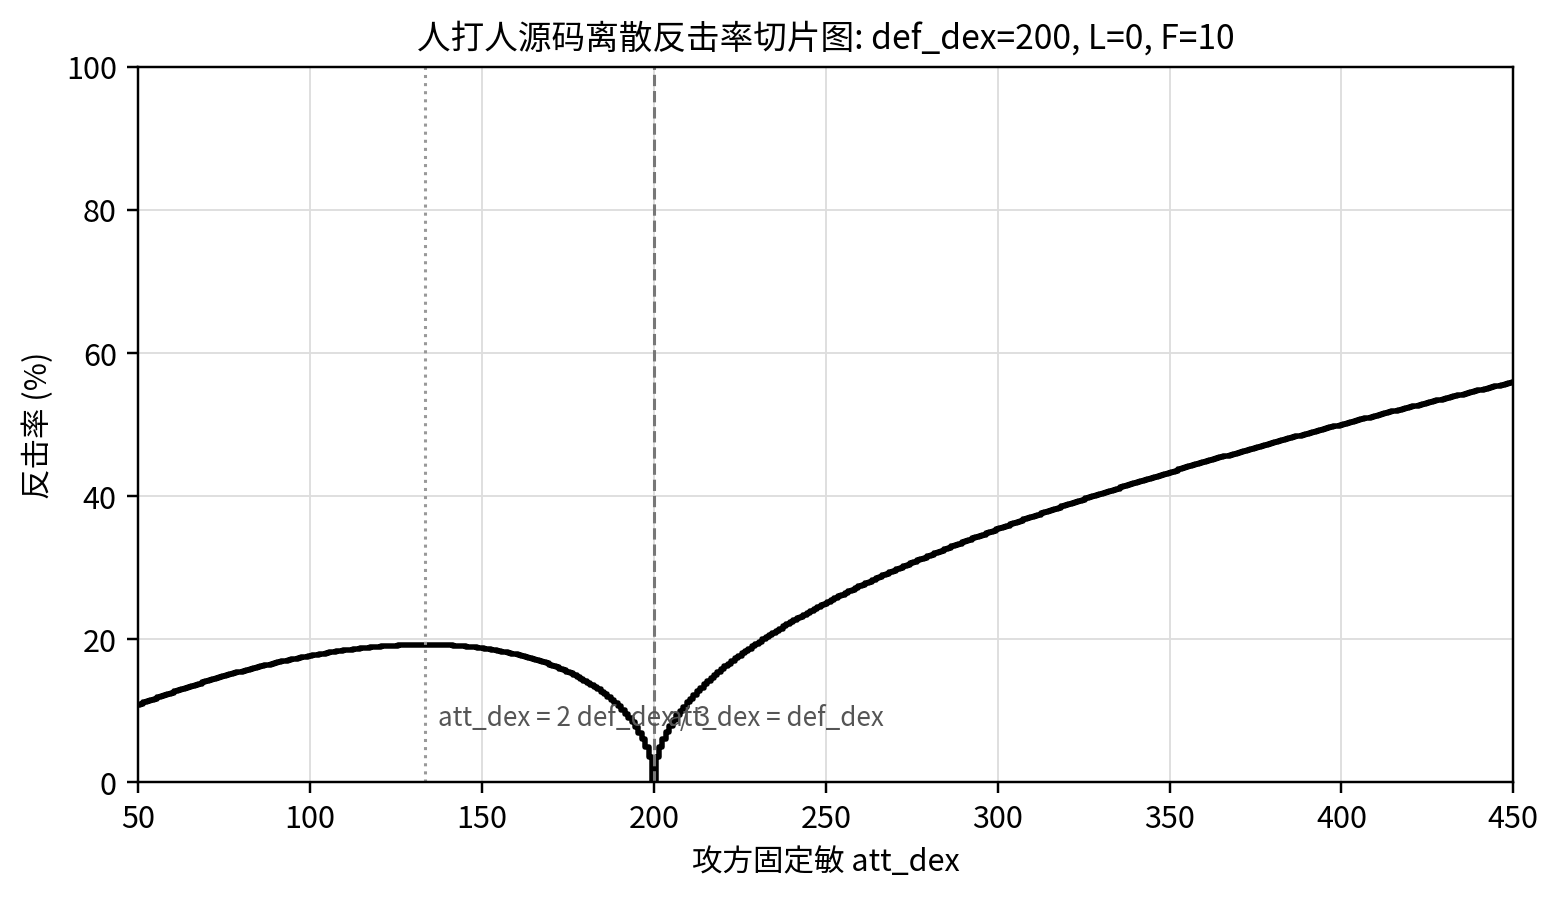
\includegraphics[width=\textwidth]{figures/counter_slice_y200_f10.png}
        \caption{反击率切片图（$F=10$）}
    \end{subfigure}
    \caption{玩家 PVP 简化口径下的源码离散切片图。统一取守方固定敏 $\defdex=200$、幸运为 $0$；会心图额外取武器会心值 $C=0$，反击图额外取武器系数 $F=10$。图中的阈值线来自连续化主体，用于标记导数符号发生变化的位置。}
    \label{fig:hit-crit-slices}
\end{figure}

从这些图可以直接看到：命中率在 $\defdex<\attdex<2\defdex$ 区间出现局部下降；会心率和反击率则都在 $2\defdex/3<\attdex<\defdex$ 区间出现局部下降。也就是说，源码中的非单调性并不是推导技巧造成的假象，而是离散数值表里可以直接观察到的结构事实。
\chapter{法术、精灵与职业技能命中机制}

物理系统和法术系统在当前源码里共用“命中/未命中”这一结果，但它们进入结果的变量层次并不相同。物理判定主要围绕固定敏和固定幸运展开，而法术系统则大量改用原始幸运、属性抗性、抗魔装备和技能熟练度。本章的目标正是把这两套命中逻辑拆开说明，并进一步解释“法术命中”和“法术伤害”为什么必须分层处理。

\section{普通属性法术命中}

普通属性法术与精灵伤害的命中入口可统一理解为 \code{BATTLE_MagicDodge()}。若目标是玩家，则未命中基数写成
\begin{equation}
    m_{\mathrm{normal}}
    = \left\lfloor 3L + 0.15R + 0.9E \right\rfloor,
    \label{eq:magic-miss-player}
\end{equation}
其中 $L$ 是目标原始幸运 \code{CHAR_LUCK}，$R$ 是目标对应属性抗性，$E$ 是抗魔装备值。法术命中率于是为
\begin{equation}
    p_{\mathrm{magic}}^{(\mathrm{player})}=100-m_{\mathrm{normal}}.
    \label{eq:magic-hit-player}
\end{equation}

若目标不是玩家，则系统不再读取幸运、抗性和抗魔装备，而改用等级近似：
\begin{equation}
    m_{\mathrm{normal}}^{(\mathrm{npc})} = \min\left\{\left\lfloor 0.2L_v \right\rfloor,\,30\right\},
\end{equation}
从而
\begin{equation}
    p_{\mathrm{magic}}^{(\mathrm{npc})}=100-m_{\mathrm{normal}}^{(\mathrm{npc})}.
\end{equation}
这两式说明了一个经常被玩家忽略的事实：普通法术打人和打宠、打怪，并不是“同一公式只换目标名字”，而是直接换了输入变量集。对玩家来说，幸运、抗性、抗魔装都重要；对非玩家单位来说，等级却成了主要近似项。还要特别指出的是，普通法术命中这一步完全不读取生命值：无论是当前生命 \code{CHAR_HP}、最大生命 \code{CHAR_WORKMAXHP}、生命成长档，还是“去掉装备修正后的生命口径”，都不进入 \code{BATTLE_MagicDodge()}。因此，生命高低本身不会改变普通法术是否命中；它只会在后续的伤害、治疗或少数以生命为基准的特殊技能里发挥作用。

\section{精灵伤害命中}

在当前实现中，精灵伤害和普通属性法术共用同一类命中入口，因此可以与式~\eqref{eq:magic-miss-player}--式~\eqref{eq:magic-hit-player} 同口径理解。也就是说，若目标是玩家，精灵是否命中主要仍由原始幸运、对应抗性和抗魔装备决定；若目标不是玩家，则主要退化为等级近似。

这意味着精灵伤害的“命中优化”空间其实很有限。进攻方通常很难像物理系那样主动堆一个明确的命中主属性，而更常见的是从守方的抗性、抗魔装和幸运入手分析减伤与抗性配置。因此，精灵命中与其说是进攻方的构筑问题，不如说更接近防守方的属性抗性问题。

\section{职业技能命中与熟练度}

职业法术命中改由职业法术闪避判定流程负责。与普通法术相比，它最重要的新增变量是对应属性熟练度。若目标是玩家，则第一段未命中基数可整理为
\begin{equation}
    m_{\mathrm{prof}}
    = \left\lfloor 3L + 0.5R + 0.4E - 0.2P \right\rfloor,
    \label{eq:prof-miss-player}
\end{equation}
其中 $L$ 为目标原始幸运，$R$ 为目标对应职业属性抗性，$E$ 为抗魔装备，$P$ 为攻方对应属性熟练度。于是第一段命中率为
\begin{equation}
    p_{\mathrm{prof},1}=100-m_{\mathrm{prof}}.
    \label{eq:prof-hit-stage1}
\end{equation}

若目标不是玩家，则幸运、装备项退化为等级近似，得到
\begin{equation}
    m_{\mathrm{prof}}^{(\mathrm{npc})}
    = \left\lfloor \min\{0.15L_v,20\} - 0.2P \right\rfloor.
\end{equation}
因此，职业法术相比普通法术多了一个清晰可控的进攻端变量 $P$。从边际结构看，玩家目标每增加 $1$ 点原始幸运会让第一段命中率约下降 $3\%$，而攻方每增加 $5$ 点熟练度会让第一段命中率约提高 $1\%$。这也是职业法术研究中“熟练度比幸运更像可优化变量”的根本原因。与普通法术一样，职业法术命中这一步同样完全不读取生命值：当前生命 \code{CHAR_HP}、最大生命 \code{CHAR_WORKMAXHP}、生命成长档，以及去掉装备修正后的生命口径，都不进入 \code{PROFESSION_MAGIC_DODGE()}；它们只会在后续伤害或特殊技能效果里发挥作用。

还必须注意一个绝对前置条件：若目标当前处于 地球一周，则职业法术会直接 Miss，不再进入式~\eqref{eq:prof-miss-player} 的概率计算。也就是说，某些防御动作并不是降低命中率，而是直接切断命中流程。

把两类法术命中并列起来，可以得到表~\ref{tab:magic-hit-compare}。

\begin{table}[H]
    \centering
    \caption{普通法术与职业法术命中的输入变量对照}
    \label{tab:magic-hit-compare}
    \begin{tabularx}{\textwidth}{>{\raggedright\arraybackslash}p{3.2cm} X X}
        \toprule
        项目 & 普通属性法术 / 精灵 & 职业法术 \\
        \midrule
        命中入口 & \code{BATTLE\_MagicDodge()} & \code{PROFESSION\_MAGIC\_DODGE()} \\
        玩家目标主要输入 & 原始幸运、对应属性抗性、抗魔装备 & 原始幸运、对应职业属性抗性、抗魔装备、攻方熟练度 \\
        非玩家目标主要输入 & 目标等级近似，最高压到 $30$ & 目标等级近似，最高压到 $20$，再减熟练度项 \\
        是否读取生命值 & 不读取 & 不读取 \\
        额外前置绝对 Miss & 无这一步 & 若目标当前动作是 \code{BATTLE\_COM\_S\_EARTHROUND0}，直接 Miss \\
        二段命中 & 无 & 部分技能存在固定二段命中 \\
        \bottomrule
    \end{tabularx}
\end{table}

\section{状态技能与二段判定}

职业技能里并不是所有法术在通过第一段命中后就直接生效。若把式~\eqref{eq:prof-hit-stage1} 的第一段命中率记为 $p_{\mathrm{prof},1}$，则部分技能还会叠加一个固定第二段命中率 $p_2$，于是最终命中率写成
\begin{equation}
    p_{\mathrm{final}} = p_{\mathrm{prof},1}\, p_2.
    \label{eq:prof-hit-stage2}
\end{equation}
当前已核对的典型二段判定包括：
\begin{equation}
    p_2=
    \begin{cases}
        0.75, & \text{电流术、暴风雨},\\
        0.90, & \text{火龙枪、世界末日},\\
        0.50, & \text{一针见血}.
    \end{cases}
\end{equation}

冰爆术则是一个非常特别的例子。源码在原本的命中分支之后又直接把 \code{hit} 重写成 $100$，因此就当前代码口径而言，这一段额外命中视为必定通过。这个例子说明，研究法术命中不能只靠技能说明文本，而必须回到实际实现顺序，因为后续覆写足以改变整段逻辑。

对状态技能而言，还要再区分“命中成功”和“状态参数如何写入”。例如四属性结界会在命中后写入结界槽位；挑拨、树根缠绕等则会继续改写攻防敏工作值。换言之，命中本身只是状态技能的入口，不是它的最终效果。

\section{命中与伤害的分层关系}

法术是否命中，与命中后造成多少伤害，是两层彼此独立的计算。若把法术基础威力记为 $M$，攻方对应熟练度记为 $P$，守方对应抗性、抗装、精灵抗性分别记为 $R,S,G$，则项目当前整理出的职业法术伤害层可写为
\begin{equation}
    damage = M\left(1+\frac{P}{100}\right)\left(1-\frac{R}{100}\right)\left(1-\frac{S}{100}\right)\left(1-\frac{G}{100}\right).
    \label{eq:magic-damage-layer}
\end{equation}
式~\eqref{eq:magic-damage-layer} 与前面的命中公式共同说明：提高法术表现有两条完全不同的路径。第一条是让 $p_{\mathrm{final}}$ 上升，也就是更容易打中；第二条是让式~\eqref{eq:magic-damage-layer} 上升，也就是打中了更疼。熟练度同时参与这两层，因此往往是职业法术里最具复合收益的进攻变量；而抗性则既能降低第一段命中，又能在命中后继续减伤，因此同样具有双重防守价值。

从研究方法看，把命中层和伤害层分开还有一个更深的意义：它让“法术最优化”不再只是一个单变量问题。若目标是稳定控场，那么提高第一段命中比堆最终伤害更重要；若目标是单次爆发，则可能宁可接受较低命中率，也要换取更高的式~\eqref{eq:magic-damage-layer}。这种目标差异在后文的优化章节中会再次出现。


\chapter{属性系统的动态变换：场地、结界、加强与反转}\label{chap:dynamic-attr}

本章只保留当前已经和源码主链直接对应、且对战斗结果有明确影响的四类机制：战场级的属性场地、单位级的四属性结界、职业技能中的属性加强，以及用标志位控制的属性反转。它们进入战斗公式的位置并不相同，因此不能混成同一类“属性状态”来理解。

\section{属性系统的整体框架}

若把一个单位在时刻 $t$ 的属性相关状态记为
\begin{equation}
    Z_t = \bigl(F_t,\;B_t,\;R_t,\;A_t\bigr),
\end{equation}
其中 $F_t$ 表示场地状态，$B_t$ 表示四属性结界，$R_t$ 表示属性反转标志，$A_t$ 表示当前生效的四属性值与抗性，那么战斗回合中的属性系统可以看成一个离散时间状态转移系统：
\begin{equation}
    Z_{t+1} = \mathcal{U}(Z_t, C_t, H_t),
\end{equation}
其中 $C_t$ 表示本回合动作集合，$H_t$ 表示本回合命中结果集合，$\mathcal{U}$ 则表示回合结算、状态写入、回合衰减与重算属性的联合算子。

这个统一写法的价值在于：它提醒我们“属性系统”不是一条公式，而是一组在不同阶段读写的状态。场地在伤害层被读取，结界在防守端减伤层被读取，属性加强若存在则应在属性重算或伤害前层进入，属性反转则在预处理重算属性时被读取。因此，若不先区分状态读写阶段，就很难解释为什么一些状态表现为覆盖，另一些却表现为开关翻转。

\section{属性场地与场地倍率}

当前真正的属性场地机制并不是职业共通技能“自我强化”，而是战场结构 \code{BattleArray[battleindex]} 上保存的场地属性、场地强度和持续回合数。若场地属性记为 $a_f$，场地强度记为 $p_f$，持续回合记为 $T_f$，则源码把它们分别写入
\begin{equation}
    \code{field_att}=a_f,\qquad \code{att_pow}=p_f,\qquad \code{att_count}=T_f.
\end{equation}

对任一单位，若其对应属性值记为 $u$，则场地倍率 \code{FieldPow} 可整理为
\begin{equation}
    \Phi(u,p_f)=0.5+\frac{up_f}{20000}.
    \label{eq:fieldpow}
\end{equation}
由于单位属性值与场地强度都不超过 $100$，所以
\begin{equation}
    0.5 \le \Phi(u,p_f) \le 1.0.
\end{equation}
当前属性伤害在经过属性相克计算之后，还会进一步乘上攻守双方场地倍率之比：
\begin{equation}
    damage_{\mathrm{field}}
    = damage_{\mathrm{attr}}
      \frac{\Phi(u_a,p_f)}{\Phi(u_d,p_f)}.
    \label{eq:field-damage}
\end{equation}
因此，场地不是单纯“给攻击方加伤”，而是通过攻守双方相对匹配度共同决定最终增减幅。

场地回合更新相对简单：每回合把 \code{att_count} 减一，当其减到非正时清空场地属性。也就是说，场地是一个战场级、单实例、按回合整体衰减的状态。

\section{四属性结界机制}

四属性结界是单位级状态，但它的存储方式与普通布尔状态不同。源码用
\begin{equation}
    \code{MAKE2VALUE(power,turn)}
\end{equation}
写入四个工作变量：
\code{CHAR_WORKFIXEARTHAT_BOUNDARY}、
\code{CHAR_WORKFIXWATERAT_BOUNDARY}、
\code{CHAR_WORKFIXFIREAT_BOUNDARY}、
\code{CHAR_WORKFIXWINDAT_BOUNDARY}。
其中高 16 位存强度 $p_b$，低 16 位存剩余回合 $T_b$。

当前实现中，结界持续回合与强度都由技能等级分档决定。若只按源码字面逻辑整理，则持续回合近似为
\begin{equation}
    T_b=
    \begin{cases}
        5, & skill\_level \ge 10,\\
        4, & skill\_level > 9,\\
        3, & skill\_level > 8,\\
        2, & skill\_level > 4,\\
        1, & \text{否则},
    \end{cases}
\end{equation}
这一分段本身存在重叠，因此更可靠的理解方式是“以代码实际执行顺序为准”，而不是按技能描述文本反推。强度则写成
\begin{equation}
    p_b=
    \begin{cases}
        100, & skill\_level \ge 100,\\
        90,  & skill\_level > 95,\\
        80,  & skill\_level > 90,\\
        70,  & skill\_level > 85,\\
        60,  & skill\_level > 80,\\
        50,  & skill\_level > 60,\\
        40,  & skill\_level > 40,\\
        30,  & skill\_level > 20,\\
        20,  & \text{否则}.
    \end{cases}
    \label{eq:boundary-power}
\end{equation}

更关键的是结界写入逻辑。若施放的是普通结界而不是“破结界”，则系统会先清掉目标侧全部四种结界，再把所选属性结界写进去。也就是说，四属性结界在当前实现里不是并存叠加关系，而是\emph{单属性覆盖关系}。若施放的是“破结界”，则会先按技能等级给一个破界成功率，成功后直接把该侧四种结界全部清空。

结界减伤公式本身也非常值得注意。若守方存在某个属性结界，则当前物理伤害分支会按攻击方对应属性值做减伤，例如土结界对应
\begin{equation}
    damage' = damage\left(1-\frac{E_a}{200}\right),
\end{equation}
其中 $E_a$ 是攻方土属性值。水、火、风结界完全类比。这里最重要的源码事实是：减伤时只检查“该结界是否存在”，实际减伤量并没有把式~\eqref{eq:boundary-power} 中存下来的 $p_b$ 再乘进去。

结界机制在实战里还有几个特别容易被误判的边界场景。第一，若同一侧已经存在某种结界，再命中另一种普通结界，则旧结界不会与新结界并存，而是先被统一清空，再由新结界覆盖写入。第二，若同一种普通结界在持续回合尚未结束时再次命中，其效果更接近“按新技能结果重写当前槽位”，而不是在旧强度、旧回合数基础上继续累加。第三，若破结界命中成功，则四种结界槽会一起清空；若失败，则原结界状态整体保留。

还可以用一个具体案例看清结界与属性反转的关系。设攻击方原始四属性记为 $(E,W,F,N)=(70,30,0,0)$，分别对应土、水、火、风；防守方身上存在土结界。若攻击方未被反转，则土结界减伤读取的是攻方当前土属性 $70$，减伤比例约为 $70/200=35\%$。若攻击方先被属性反转，则当前有效属性会变成 $(0,0,70,30)$。此时防守方虽然仍是”土结界”，但减伤读取的已经是反转后的土属性 $0$，减伤比例下降为 $0/200=0\%$。这说明结界槽位本身不会被反转交换，但它所读取的”攻方对应属性值”会随着反转后的当前属性而改变。

同理，场地倍率也应理解为读取“当回合生效属性”而不是角色的某个静态建档值。若某单位长期带有属性反转标志，则其每回合预处理后参与场地倍率计算的属性向量也会是反转后的版本。于是，属性反转不仅会改变属性相克和结界减伤，还会连带改变该单位在场地中的受益方向。

\section{属性加强机制}

这一节的结论非常简单，但必须明确写出来：当前源码中的职业共通技能“属性加强（自我强化）”对应实现仅返回 \code{TRUE}，没有看到实际数值逻辑。也就是说，就这份代码口径而言，“自我强化”的战斗内数值效果是\emph{空实现}。

这件事的重要性不在于“某个技能没写完”，而在于它提醒研究不能把玩家经验中的效果自动补回源码。若后续版本或别的分支实现了具体公式，那应当另行分析；但在当前论文口径下，属性加强只能被记为“在现有源码中未见明确数值作用”，而不能擅自假定为乘法、加法或覆盖效果。进一步说，这也意味着几个常见的边界猜想在当前代码下都不成立：多次施放属性加强不会形成层数累加，属性加强也不会与结界、场地或属性反转再叠出额外乘区，因为源码里根本没有可供叠加的数值入口。

\section{属性反转机制}

属性反转的实现是本章最需要按时序理解的部分。技能命中后，系统先对目标的 \code{CHAR_BATTLEFLG_REVERSE} 做一次异或：
\begin{equation}
    flg \leftarrow flg \oplus \code{REVERSE},
\end{equation}
然后立即调用 \code{BATTLE_AttReverse()}。后者并不是“无条件再交换一次”，而是先检查目标头上当前是否仍带有 \code{REVERSE} 标记；只有标记存在时，才把当前固定属性按如下映射交换：
\begin{equation}
    (E,W,F,N) \longmapsto (F,N,E,W),
    \label{eq:reverse-map}
\end{equation}
其中 $E,W,F,N$ 分别表示土、水、火、风。也就是说，土火互换，水风互换。

这个判定顺序会带来一个很关键的结论。第一次命中属性反转时，标记从关变开，于是 \code{BATTLE_AttReverse()} 会立刻把当前固定属性切到反转态。第二次命中同技能时，标记从开变关；这时 \code{BATTLE_AttReverse()} 进入后会直接返回，因此\emph{不会在命中当下把当前固定属性切回原态}。也就是说，“反转标记被关掉”和“当前固定属性立刻复原”在源码里不是同一件事。

真正把属性恢复成正常口径的，是后续的固定属性重算过程。在每回合预处理 \code{BATTLE_PreCommandSeq()} 中，系统会先重算本回合固定属性；只有头上仍带有 \code{REVERSE} 标记时，才会再次调用 \code{BATTLE_AttReverse()}。因此，若某单位已经处于反转态，又在同回合再次被属性反转命中，则会出现一个临时状态：\emph{标记已经被清掉，但当前这份固定属性快照仍然保持反转结果}。等到下一次固定属性重算发生时，由于标记已关，系统不再补做交换，属性才会回到正常口径。

这也正是前一版文稿里“连续两次命中就会立刻切回原态”不成立的原因。更准确的说法应当是：第二次命中会关掉反转标记，但不会立即重做一次逆交换；是否在同回合内就恢复正常，要看之后是否还有新的固定属性重算入口。若没有，就会把这份反转后的固定属性继续用到本回合后续判定里；若有，则会在那次重算后恢复成正常属性。

这一机制可以直接推出几个边际案例。第一，若单位在反转状态尚未解除时更换装备、骑宠状态改变，或本回合又被其它流程重写固定属性，则下一次重算会先按最新口径生成固定属性，再根据标记是否仍在决定要不要继续交换。因此，反转作用的是“当回合有效属性”，不是“某次命中时刻留下来的旧快照”。第二，若防守方处于反转状态而攻击方施放结界，结界写入的仍然是土、水、火、风四个固定槽位本身；被交换的是人物当前属性，而不是结界槽位的语义。换言之，反转会改变结界减伤读取到的属性值，但不会把“土结界”变成“火结界”。第三，若同一目标在同回合内先被反转、后又被同技能再次命中，就可能出现“头上已无反转标记，但当前属性仍按反转态参与余下判定”的过渡现象；这正是需要把“标记状态”和“当前固定属性快照”分开理解的地方。

从玩家语言看，常把这类效果叫作“属性转换”。本文沿用源码口径称其为“属性反转”，原因就在于它不是把某一项属性永久改写成另一项，而是通过一个可开可关的标志位，在固定属性重算之后对当前属性做映射交换。这个差异看似只是命名问题，实则决定了我们应该把它理解成一个“标记控制的重算后交换过程”，而不是一次性的数值替换。

\section{多次状态命中的属性演化}

把前几节合起来看，可以把多次状态命中分成三种完全不同的演化模式。

第一种是\emph{覆盖型}，代表就是四属性结界。普通结界命中后会先清空已有四结界，再写入新结界，因此新状态会覆盖旧状态，而不是叠加在旧状态之上。第二种是\emph{翻转型}，代表是属性反转，但这里的“翻转”严格地说只发生在标志位层；至于当前固定属性是否立刻改回去，还要看当下有没有重新进入属性重算。第三种是\emph{回合重算型}，代表属性场地、结界剩余回合以及当前固定属性本身，它们会在回合推进时统一进入新的状态快照。

从目前已核对的代码可确定：结界的“多次命中”不是强度叠加而是覆盖；反转的“多次命中”不是刷新持续时间，而是对反转标志做异或；破结界的“多次命中”则表现为若干次独立清空尝试。更细一点地说，若同回合内先后发生“普通结界命中、破结界命中、再一次普通结界命中”，则最终保留的是最后一次成功写入的普通结界；若同回合内属性反转连续命中两次，则最终的标记状态会回到关闭，但当前固定属性是否已经恢复，还要看是否发生过新的固定属性重算；若同回合内既有反转又有结界，则结界写入的是槽位，反转影响的是之后读取这些槽位时所对应的当前属性值。这些都是典型的“顺序敏感”案例。

\section{动态属性系统的状态转移模型}

综合前述各节，当前属性系统最适合写成由若干算子组成的离散更新链。若把场地算子记为 $\mathcal{F}$，结界写入算子记为 $\mathcal{B}$，反转标志与属性交换的联合算子记为 $\mathcal{R}$，回合衰减算子记为 $\mathcal{D}$，则一回合内的属性状态更新可抽象为
\begin{equation}
    Z_{t+1}
    = \mathcal{D}\circ \mathcal{R}^{\mathbf{1}_{\mathrm{reverse}}}
      \circ \mathcal{B}^{\mathbf{1}_{\mathrm{boundary}}}
      \circ \mathcal{F}^{\mathbf{1}_{\mathrm{field}}}(Z_t),
\end{equation}
其中各指标函数表示本回合是否有相应状态命中。虽然这只是抽象写法，但它足以揭示三个关键结论。

第一，属性系统不是交换群结构，不同状态写入顺序不可随意交换。例如结界是在防守端减伤层生效，而反转是在固定属性重算后生效，因此“先反转再上结界”和“先上结界再反转”不一定等价。第二，反转的可逆性成立于“标志位层”和“完整重算后的新属性快照层”，不能粗暴理解成“连续命中两次就立刻把当前值切回去”。第三，所谓“属性玩法”并不是单一伤害乘法，而是一套由战场级状态、单位级状态和标志位共同构成的动态系统。这一视角也正是后文把宠物培养、骑宠速度、法术命中与伤害统一到同一研究框架中的关键桥梁。

\chapter{骑宠、攻防混合与最终伤害公式}

本章讨论战斗系统中另一个容易被经验说法简化过度的部分：骑宠状态下，人物与宠物的攻击、防御、敏捷究竟如何混合；而这种混合又如何继续进入物理伤害、属性修正与会心附加伤害。若只看面板，很容易误以为骑宠只是“骑上去加一点能力”；但从源码角度看，骑宠实际上改变了多个核心变量的来源层级，因此它不仅影响数值大小，也改变了数值进入公式的路径。

\section{骑宠攻击力与防御力混合}

在当前研究口径下，骑宠三围的读取主要对应 \code{BATTLE_adjustRidePet3A()}，并以前文已说明的 \code{_BATTLE_NEWPOWER} 分支为主。这里首先要区分是否装备远程武器，因为远程和近战的混合方式并不相同。

设人物攻击力、防御力分别为 $A_c,D_c$，骑宠攻击力、防御力分别为 $A_p,D_p$。若攻击方未骑宠，则物理攻击直接取
\begin{equation}
    A = A_c.
\end{equation}
若攻击方已骑宠，则当装备远程武器时，攻击力混合为
\begin{equation}
    A = A_c + 0.4A_p,
    \label{eq:ride-atk-ranged}
\end{equation}
而当装备近战武器或空手时，攻击力混合为
\begin{equation}
    A = 0.8A_c + 0.8A_p.
    \label{eq:ride-atk-melee}
\end{equation}
式~\eqref{eq:ride-atk-ranged} 与式~\eqref{eq:ride-atk-melee} 的差异说明，骑宠近战并不是单纯“由宠物代打”，而是人物与宠物攻击共同占据较高权重；相反，骑宠远程则明显偏向人物本体，只把宠物作为额外附加项。

防御侧的结构更特殊。若防守方未骑宠，则在 \code{BATTLE_DamageCalc()} 中会先取
\begin{equation}
    D = 0.70D_c.
    \label{eq:def-no-ride}
\end{equation}
若防守方已骑宠，则首先在骑宠混合函数中得到
\begin{equation}
    D_{ride}=0.7D_c+0.7D_p,
\end{equation}
随后再进入伤害函数乘以一次 $0.70$，于是最终用于物伤计算的防御量为
\begin{equation}
    D = 0.70D_{ride}=0.49D_c+0.49D_p.
    \label{eq:def-ride}
\end{equation}
因此，在当前编译口径下，骑宠防御既不是人物防御与宠物防御的简单平均，也不是只取宠物，而是对两者做同权线性组合后再统一衰减一次。

\section{骑宠敏捷混合}

骑宠敏捷的处理与攻击、防御不同，它必须区分“攻击侧读取”与“防守侧读取”，还必须区分远程武器与近战武器。设人物战斗速度敏为 $Q_c$，骑宠战斗速度敏为 $Q_p$。则在攻击侧，若使用远程武器，读取为
\begin{equation}
    Q_{atk}^{(ranged)} = 0.8Q_c + 0.2Q_p,
    \label{eq:ride-quick-ranged}
\end{equation}
若使用近战武器或空手，则读取为
\begin{equation}
    Q_{atk}^{(melee)} = 0.2Q_c + 0.8Q_p.
    \label{eq:ride-quick-melee}
\end{equation}
而在防守侧，读取进一步偏向宠物，写成
\begin{equation}
    Q_{def} = 0.1Q_c + 0.9Q_p.
    \label{eq:ride-quick-def}
\end{equation}
这说明骑宠并不仅仅改变“谁出手”，还改变“速度由谁主导”。从直觉上说，骑宠近战明显更偏宠物，骑宠远程明显更偏人物，而骑宠防守几乎可以看作宠物敏捷主导。正因为如此，同一只宠物在“骑近战”和“骑远程”两种配置下，既可能表现出完全不同的先手性质，也可能在后续伤害、命中与反击中体现出不同的角色定位。

\section{物理伤害三段式公式}

设前两节得到的攻击量与防御量分别记为 $A$ 与 $D$。在当前 \code{_BATTLE_NEWPOWER} 分支下，物理伤害的基础体可分成三段。若
\begin{equation}
    D > A,
\end{equation}
则基础物伤只在极低范围内波动，可整理为
\begin{equation}
    damage = \operatorname{RAND}(0,1).
    \label{eq:damage-stage1}
\end{equation}
若
\begin{equation}
    D \le A < \frac{8}{7}D,
\end{equation}
则进入第二段：
\begin{equation}
    damage = \operatorname{RAND}\left(0,\frac{A}{16}\right).
    \label{eq:damage-stage2}
\end{equation}
若
\begin{equation}
    A \ge \frac{8}{7}D,
\end{equation}
则进入第三段，记
\begin{equation}
    K_0 = \operatorname{RAND}\left(0,\frac{A}{8}\right)-\frac{A}{16},
\end{equation}
则基础物伤为
\begin{equation}
    damage = 2(A-D)+K_0.
    \label{eq:damage-stage3}
\end{equation}
其中当前源码常量对应
\begin{equation}
    DAMAGE\_RATE=2.0, \qquad D\_8=\frac{1}{8}, \qquad D\_{16}=\frac{1}{16}.
\end{equation}
从结构上看，式~\eqref{eq:damage-stage1}--\eqref{eq:damage-stage3} 构成了一个典型的分段物伤模型：当攻击显著低于防御时，伤害几乎被压到 $0$ 或 $1$；当攻击刚刚接近防御时，仍停留在小幅随机区间；只有当攻击高于 $8D/7$ 之后，伤害才开始表现为对 $(A-D)$ 的线性函数并叠加轻微随机扰动。

\section{防御动作、全防与偏转的介入顺序}

除了前文的防御力工作值以外，当前物理伤害流程里还存在一条独立的“防御链”。它不直接改写 \code{CHAR_WORKDEFENCEPOWER}，而是在基础伤害已经算出之后，再按动作状态或专门判定去压低最终伤害。

其中最基础的一层是\emph{防御动作}。若防守方当前动作是 \code{BATTLE_COM_GUARD}，且未处于混乱，则源码不会简单按固定比例减伤，而是调用 \code{BATTLE_GuardAdjust()} 做一次六档随机压缩：
\begin{equation}
    damage_{guard} \in \{0,0.1,0.2,0.3,0.4,0.5\}\cdot damage,
\end{equation}
其概率分布分别为
\begin{equation}
    (25\%,25\%,20\%,15\%,10\%,5\%).
\end{equation}
也就是说，防御并不是“固定减半”，而是以完全挡下到保留一半伤害之间的离散随机分布实现。若压缩后伤害降到 $0$，系统还会继续把这次结果标记为 \code{BATTLE_RET_ALLGUARD}，在表现层显示为防御成功。

第二层是\emph{偏转 / 招架}。若编译路径启用了 \code{_EQUIT_ARRANGE}，则在普通防御动作之外，还会额外调用 \code{BATTLE_ArrangeCheck()}。一旦成立，本次伤害会被直接压到原值的 $10\%$，并返回独立的偏转结果码。对玩家阅读而言，这一层更接近“招架成功后大幅卸力”，而不是普通防御动作本身。

第三层是\emph{忽视防御}。若编译路径启用了 \code{_EQUIT_NEGLECTGUARD}，且攻击方装备或状态给出了 \code{CHAR_WORKNEGLECTGUARD}，则它并不是去跳过“防御动作”，而是在基础物伤计算前先按比例削减防守方防御量。若忽视防御比例记为 $r\%$，则进入物伤公式的防御量会先变成
\begin{equation}
    D' = \left(1-\frac{r}{100}\right)D.
\end{equation}
因此，忽视防御影响的是三段式物伤的分段位置，而不是后面的防御动作随机压缩。

把这几层放到同一条顺序里，可以更准确地写成：先由攻击力与防御力工作值得到基础物伤，再经过属性修正与结界减伤，然后再检查防御动作、偏转和伤害反应等后置环节。于是，玩家口中的“被格挡了”在源码里其实可能对应三种完全不同的机制：普通防御动作的随机减伤、偏转 / 招架的 $10\%$ 压缩，或吸收 / 反射 / 消失等伤害反应。它们在日志表现上都可能让单次伤害显著下降，但进入公式的位置并不相同。


\section{属性克制、场地倍率与结界减伤}

基础物伤只是整个伤害流程的第一层。对当前实现而言，式~\eqref{eq:damage-stage1}--\eqref{eq:damage-stage3} 得到的结果还要继续经过属性克制、场地倍率与结界减伤，然后才进入额外扰动与后续表现层。与很多玩家经验不同，这一段并不是“看主属性相克后乘一个固定倍率”，而是一个由\emph{五维属性向量、双线性相克矩阵与场地比值}共同组成的计算链。

\subsection{攻击方与防守方的五维属性向量}

在当前 \code{_BATTLE_NEWPOWER} 口径下，物理伤害使用的属性值由 \code{BATTLE\_GetAttr()} 直接从单位自身的四属性工作值读取，而不会因为骑宠状态再把人物与宠物属性做一次平均。也就是说，骑宠会混合攻击、防御与敏捷，但\textbf{不会在当前主分支里混合物理属性向量}。若把攻击方四属性写成
\begin{equation}
    (p_E,p_W,p_F,p_{Wi}),
\end{equation}
把防守方四属性写成
\begin{equation}
    (q_E,q_W,q_F,q_{Wi}),
\end{equation}
则源码会先把负值裁到 $0$，再补出无属性分量
\begin{equation}
    p_N = \max\{100-p_E-p_W-p_F-p_{Wi},0\},
    \qquad
    q_N = \max\{100-q_E-q_W-q_F-q_{Wi},0\}.
    \label{eq:none-attr}
\end{equation}
于是攻守双方真正进入属性克制计算的，分别是五维向量
\begin{equation}
    \bm{p}=(p_E,p_W,p_F,p_{Wi},p_N),
    \qquad
    \bm{q}=(q_E,q_W,q_F,q_{Wi},q_N).
\end{equation}

式~\eqref{eq:none-attr} 说明，只要四属性之和没有达到 $100$，剩余部分就会自动落入无属性；若四属性和已经超过 $100$，则无属性被截成 $0$，而不会出现负的无属性值。

\subsection{属性克制的源码矩阵}

记式~\eqref{eq:damage-stage1}--\eqref{eq:damage-stage3} 的基础物伤为 $damage_0$。源码会先把攻击方五维属性按比例拆到这份基础物伤上，再与防守方五维属性逐项相乘，并乘上三种常量
\begin{equation}
    AJ_{\mathrm{up}}=1.5,
    \qquad
    AJ_{\mathrm{same}}=1.0,
    \qquad
    AJ_{\mathrm{down}}=0.6.
\end{equation}
若按 $(E,W,F,Wi,N)$ 的顺序排列攻守属性，则源码等价于使用如下相克矩阵
\begin{equation}
    M=
    \begin{bmatrix}
        1.0 & 1.5 & 1.0 & 0.6 & 1.5 \\
        0.6 & 1.0 & 1.5 & 1.0 & 1.5 \\
        1.0 & 0.6 & 1.0 & 1.5 & 1.5 \\
        1.5 & 1.0 & 0.6 & 1.0 & 1.5 \\
        0.6 & 0.6 & 0.6 & 0.6 & 1.0
    \end{bmatrix}.
    \label{eq:attr-matrix}
\end{equation}
于是属性克制后的物伤主体可以直接写成
\begin{equation}
    damage_{\mathrm{attr}}
    = damage_0\,\frac{\bm{p}^{\mathsf T}M\bm{q}}{10000}.
    \label{eq:damage-attr-core}
\end{equation}

式~\eqref{eq:attr-matrix} 给出的口径有几个实战上很容易记反的点。其一，土克水、水克火、火克风、风克土；相克链并不是很多玩家口口相传的另一种写法。其二，同属性与“隔一位”的属性关系在当前物伤克制里都按 $1.0$ 处理。其三，\emph{无属性并不是中立常数}：元素打无属性按 $1.5$ 算，无属性打任意元素按 $0.6$ 算，只有无属性打无属性才是 $1.0$。

若只看纯属性对纯属性，则式~\eqref{eq:damage-attr-core} 可以压缩成表~\ref{tab:physical-attr-pure}。

\begin{table}[H]
    \centering
    \caption{物理伤害中纯属性对纯属性的源码倍率}
    \label{tab:physical-attr-pure}
    \begin{tabularx}{\textwidth}{>{\raggedright\arraybackslash}p{1.8cm} *{5}{>{\centering\arraybackslash}X}}
        \toprule
        攻 \textbackslash{} 守 & 土 & 水 & 火 & 风 & 无 \\
        \midrule
        土 & $1.0$ & $1.5$ & $1.0$ & $0.6$ & $1.5$ \\
        水 & $0.6$ & $1.0$ & $1.5$ & $1.0$ & $1.5$ \\
        火 & $1.0$ & $0.6$ & $1.0$ & $1.5$ & $1.5$ \\
        风 & $1.5$ & $1.0$ & $0.6$ & $1.0$ & $1.5$ \\
        无 & $0.6$ & $0.6$ & $0.6$ & $0.6$ & $1.0$ \\
        \bottomrule
    \end{tabularx}
\end{table}

\subsection{场地倍率不是加法，而是攻守比值}

属性克制并不是这一层的终点。源码接着会读取战场属性 \code{field\_att} 与场地强度 \code{att\_pow}，分别对攻击方与防守方算一次场地倍率，然后取二者比值乘回伤害。设当前场地属性为 $X\in\{E,W,F,Wi\}$，场地强度为 $s$，则对任意一方属性向量 $\bm{u}$，其场地倍率可写成
\begin{equation}
    \phi_X(\bm{u}) = 0.5 + 0.5\,u_X\,\frac{s}{10000},
    \label{eq:field-ratio}
\end{equation}
若当前没有属性场地，则源码回到默认值
\begin{equation}
    \phi_{\mathrm{none}}(\bm{u}) = 0.5.
\end{equation}
于是属性与场地共同作用后的结果是
\begin{equation}
    damage_1 = damage_{\mathrm{attr}}\,\frac{\phi_X(\bm{p})}{\phi_X(\bm{q})}.
    \label{eq:damage-after-field}
\end{equation}

式~\eqref{eq:damage-after-field} 的一个直接推论是：场地不是简单给攻击方加成，也不是简单给防守方减伤，而是对攻守双方\emph{同时各算一次倍率再取比值}。因此，同一个火场里，火高的攻击方确实会放大输出，但火高的防守方也会通过分母把这部分收益抵消掉一部分。

\subsection{四属性结界的减伤公式}

在 \code{_PROFESSION_ADDSKILL} 分支下，物伤经过式~\eqref{eq:damage-after-field} 后，还会再检查防守方是否挂有四属性结界。这里的实现有三个值得单独指出的源码细节。

第一，结界检查是按
\begin{equation}
    E \rightarrow W \rightarrow F \rightarrow Wi
\end{equation}
的 \code{if-else if} 顺序进行，因此同一时刻即使理论上挂了多个结界，也只会命中第一条成立的分支。第二，减伤读取的是\emph{攻击方原始固定属性工作值}，而不是式~\eqref{eq:damage-after-field} 里已经参与过场地和相克计算的属性向量。第三，结界高位里存放的“强度值”在当前物伤减伤公式中并不直接进入比例，只起到“该结界是否开启”的开关作用。

若记命中的结界属性为 $k\in\{E,W,F,Wi\}$，记攻击方对应的固定属性工作值为 $r_k$，则当前源码下的结界减伤可写成
\begin{equation}
    damage_2 = damage_1\left(1-\frac{r_k}{200}\right).
    \label{eq:boundary-reduce}
\end{equation}
若没有任何结界成立，则直接有
\begin{equation}
    damage_2 = damage_1.
\end{equation}

式~\eqref{eq:boundary-reduce} 说明，结界并不是“固定减半”或“按结界强度减伤”，而是按攻击方同属性点数做线性压缩。例如攻击方火属性固定值为 $40$，而防守方当前触发的是火结界，则物伤会再乘上 $1-40/200=0.8$。

\subsection{属性反转如何进入本章伤害公式}

第~\ref{chap:dynamic-attr} 章已经说明，属性反转并不是直接改写某个“永久主属性”，而是通过标志位控制当前固定属性快照的交换。在伤害层面，这意味着它影响的不是某个后置乘区，而是本节前面几条公式的\emph{输入量本身}。

若某单位当前有效固定属性由式~\eqref{eq:reverse-map} 从
\begin{equation}
    (E,W,F,Wi) \longmapsto (F,Wi,E,W)
\end{equation}
交换而来，那么在当前主分支下至少有三处会随之改变。

第一，\code{BATTLE\_GetAttr()} 读取到的攻击方或防守方属性向量 $\bm{p},\bm{q}$ 会改成反转后的版本，因此式~\eqref{eq:damage-attr-core} 中的双线性相克值会整体改变。第二，式~\eqref{eq:field-ratio} 中用于计算场地倍率的对应属性分量 $u_X$ 也会改成反转后的版本，因此同一块场地上的攻守比值可能随反转而跳变。第三，式~\eqref{eq:boundary-reduce} 中的 $r_k$ 直接读取攻击方当前固定属性工作值，所以结界减伤也会跟着反转后的属性一起变化。

因此，若把“反转前”的伤害记为
\begin{equation}
    damage_2 = \mathcal{D}(\bm{p},\bm{q},r_k),
\end{equation}
把“反转后”的伤害记为
\begin{equation}
    damage_2^{(rev)} = \mathcal{D}(\bm{p}^{(rev)},\bm{q}^{(rev)},r_k^{(rev)}),
\end{equation}
则差异不止发生在某一步，而是会同时穿过
\begin{equation}
    \bm{p}^{\mathsf T}M\bm{q},
    \qquad
    \frac{\phi_X(\bm{p})}{\phi_X(\bm{q})},
    \qquad
    1-\frac{r_k}{200}
\end{equation}
这三层结构。

这里还要补一个只从第十章公式本身不容易看出的时序细节。当前物伤函数并不重新检查“反转标志此刻是开是关”，它只读取\emph{当前这份已经算好的固定属性工作值}。因此，若出现第~\ref{chap:dynamic-attr} 章讨论过的过渡情形，即“反转标志已经被清掉，但新的固定属性重算尚未发生”，那么本章中的 $\bm{p},\bm{q},r_k$ 仍会继续使用那份尚未恢复的反转态快照。这也是一些实战现象看上去像“反转效果多保留了一段时间”的根源。

\subsection{两个完整算例}

为了避免把式~\eqref{eq:damage-attr-core}--\eqref{eq:boundary-reduce} 看成抽象符号，这里给出两个按当前源码口径直接展开的例子。

\paragraph{例 1：属性克制与场地比值共同放大伤害}
设基础物伤 $damage_0=120$，攻击方属性向量为 $\bm{p}=(60,20,10,0,10)$，防守方属性向量为 $\bm{q}=(10,50,20,0,20)$，当前为土场地，场地强度 $s=80$。按式~\eqref{eq:damage-attr-core} 与式~\eqref{eq:damage-after-field} 展开，可把关键中间量压缩成表~\ref{tab:damage-example-field}。

\begin{table}[H]
    \centering
    \caption{算例 1：属性克制与土场地的联合放大}
    \label{tab:damage-example-field}
    \begin{tabularx}{\textwidth}{>{\raggedright\arraybackslash}p{3.0cm} X >{\raggedleft\arraybackslash}p{2.7cm}}
        \toprule
        步骤 & 计算内容 & 结果 \\
        \midrule
        基础物伤 & 已知 $damage_0$ & $120$ \\
        属性克制主体 & $\bm{p}^{\mathsf T}M\bm{q}$ & $12000$ \\
        属性克制后伤害 & $120\times 12000/10000$ & $144$ \\
        攻方土场倍率 & $0.5+0.5\times 60\times 80/10000$ & $0.74$ \\
        守方土场倍率 & $0.5+0.5\times 10\times 80/10000$ & $0.54$ \\
        场地修正后伤害 & $144\times 0.74/0.54$ & $\approx 197.33$ \\
        \bottomrule
    \end{tabularx}
\end{table}

这个例子说明，属性克制已经先把伤害从 $120$ 推高到 $144$，而土场地又因为攻击方土属性显著高于防守方土属性，继续把伤害推到约 $197.33$。也就是说，场地收益并不是单独存在的，它会在属性克制已经放大的基础上继续按攻守比值放大。

\paragraph{例 2：属性反转同时改变场地收益与结界减伤}
设基础物伤 $damage_0=100$，防守方为纯无属性 $\bm{q}=(0,0,0,0,100)$，当前为火场地、场地强度 $s=100$，且防守方身上存在土结界。攻击方反转前的当前固定属性为 $\bm{p}=(80,20,10,5,0)$，按第~\ref{chap:dynamic-attr} 章的反转映射，反转后的当前固定属性变为 $\bm{p}^{(rev)}=(10,5,80,20,0)$。关键中间量汇总见表~\ref{tab:damage-example-reverse}。

\begin{table}[H]
    \centering
    \caption{算例 2：属性反转如何同时改写场地与结界}
    \label{tab:damage-example-reverse}
    \begin{tabularx}{\textwidth}{>{\raggedright\arraybackslash}p{3.1cm} >{\raggedleft\arraybackslash}X >{\raggedleft\arraybackslash}X}
        \toprule
        步骤 & 反转前 & 反转后 \\
        \midrule
        攻方当前属性 & $(80,20,10,5,0)$ & $(10,5,80,20,0)$ \\
        属性克制后伤害 $damage_{\mathrm{attr}}$ & $172.5$ & $172.5$ \\
        火场攻方倍率 & $0.55$ & $0.9$ \\
        火场守方倍率 & $0.5$ & $0.5$ \\
        场地修正后伤害 $damage_1$ & $189.75$ & $310.5$ \\
        土结界读取的攻方土属性 & $80$ & $10$ \\
        结界修正后伤害 $damage_2$ & $113.85$ & $294.975$ \\
        \bottomrule
    \end{tabularx}
\end{table}

这个例子非常典型：反转前后，属性克制主体本身没有变，但火场地倍率和土结界减伤同时被改写，最终伤害仍然从 $113.85$ 大幅跳到约 $294.98$。因此，实战里看到“反转后伤害忽然暴涨”，并不一定意味着攻防差或会心出了问题，很多时候只是属性向量在场地与结界两个层面同时改了方向。

\subsection{把属性层并入最终伤害顺序}

把本章前文与本节合并后，当前主分支下的物理伤害顺序可以整理为
\begin{equation}
    damage_0
    \xrightarrow{\text{属性克制矩阵}}
    damage_{\mathrm{attr}}
    \xrightarrow{\text{场地比值}}
    damage_1
    \xrightarrow{\text{四属性结界}}
    damage_2
    \xrightarrow{\text{额外扰动}}
    damage_3.
\end{equation}
其中若编译启用了额外伤害与额外减伤系统，则附加扰动写成
\begin{equation}
    \Delta_{extra} = \operatorname{RAND}(0.3P_a,P_a)-\operatorname{RAND}(0.3P_d,P_d),
\end{equation}
并有
\begin{equation}
    damage_3 = \max\{damage_2 + \Delta_{extra},0\}.
\end{equation}

这样一来，完整的物伤主体就不应再被理解成“攻防差后乘一个属性修正”。更准确地说，它是“\textbf{攻防分段函数 + 五维属性双线性克制 + 场地攻守比值 + 结界线性减伤 + 额外扰动}”的串联结构。特别是在骑宠环境下，攻击、防御会跟随骑宠混合，但属性向量仍读取当前单位自身工作值；这意味着“骑宠面板变了”与“属性克制结果变了”在源码里是两件相互独立的事情。

\section{会心额外伤害}

会心成立之后，伤害并不是直接乘以某个固定倍率。对当前实现而言，若武器不是弓，则系统先按普通流程算出基础物伤，再额外增加一段由防守方防御与双方等级共同决定的附加伤害。记普通物伤结果为 $damage$，攻击方等级与防守方等级分别为 $L_a$ 与 $L_d$，则会心附加后的结果可整理为
\begin{equation}
    damage_{crit} = damage + 0.5\,DEF_c\frac{L_a}{L_d},
    \label{eq:crit-damage}
\end{equation}
其中 $DEF_c$ 表示防守方的防御力工作值。式~\eqref{eq:crit-damage} 说明，会心本质上是“普通物伤 + 一段额外防御比例项”，而不是传统 RPG 中常见的“普通物伤乘一个暴击倍数”。

这一点对实战理解非常关键。若玩家只根据最终伤害浮动去猜测机制，往往会误以为会心是一个乘法型收益；但在当前源码口径下，会心的附加量与防守方防御及双方等级比直接相关，因此对不同目标的收益会显著不同。防高、等级低的目标可能吃到更大的会心附加，而防低、等级接近的目标则未必体现出同样夸张的增幅。进一步地，弓虽然仍可判出会心事件，但不会调用这段附加伤害函数，因此弓系配置在概率层面的会心和在爆发层面的会心并不是同一件事。

\section{变量影响分析}

\subsection{攻击对伤害的边际收益是分段的}

由式~\eqref{eq:damage-stage1}--\eqref{eq:damage-stage3} 可见，攻击力提升的边际收益并不是全局平滑递增的。当 $A<D$ 时，提高攻击的主要效果只是让随机区间从“几乎固定为 $0$ 或 $1$”逐步靠近第二段，边际收益非常弱；当 $D\le A < 8D/7$ 时，伤害上界随 $A/16$ 线性增加，但仍停留在小区间随机；只有跨过 $8D/7$ 这条阈值后，攻击提升才开始几乎按 $2(A-D)$ 的斜率进入主导区间。因此，若某个配置长期处在第二段附近，那么继续加攻击的体感收益可能远低于玩家的线性预期。

\subsection{骑宠远程与骑宠近战的收益结构不同}

由式~\eqref{eq:ride-atk-ranged} 与式~\eqref{eq:ride-atk-melee} 可知，骑宠远程与骑宠近战并不是“同一公式换个武器名字”。远程侧更偏人物攻击，近战侧则让人物和宠物都以较高权重进入攻击项；同时，敏捷侧又分别服从式~\eqref{eq:ride-quick-ranged} 与式~\eqref{eq:ride-quick-melee}。这意味着在骑宠配置下，“提高宠物攻击”与“提高宠物敏捷”的收益取决于你最终打算走远程还是近战，不能脱离武器类型单独讨论。

\subsection{防御与石化、忽视防御等状态的作用顺序}

防御量在进入伤害三段式之前，还可能受到铁壁防御、石化、无装备防御和忽视防御等状态影响。由于这些修正发生在不同位置，它们的实际效果并不相同。石化会直接把防御翻倍，从而整体抬高第三段门槛；忽视防御则在防御量已经形成之后再按比例削减，因此更接近对门槛的整体下压；若存在无装备防御类技能，则防御甚至会被直接替换为另一套工作值。由此可见，战斗中的“防御变化”并不只是某个数值加减，而是可能改变整条分段函数所处区间。

综上，骑宠与物伤系统共同呈现出一个高度离散、分段且带路径依赖的结构。攻击、防御、武器类型、骑宠状态、属性结界和会心并不是独立叠加，而是按特定顺序进入不同层级的公式。对于论文后续章节而言，这一结构恰好提供了一个桥梁：前文宠物成长与喂药所产生的数值差异，最终正是通过本章这些分段函数与混合公式，转化为实战中的先手、压制、爆发与承伤差异。

\chapter{宠物养成对战斗能力的映射}

前文已经分别讨论了宠物成长、转生、融合、蛋喂药、乱敏、命中、会心和骑宠伤害。真正的研究价值并不在于这些部分各自成立，而在于它们能否被接成一条从“养成输入”到“战斗输出”的完整链条。本章的任务正是把这条链条显式写出来：宠物的成长率如何转化为攻击、防御、敏捷；转生、融合和喂药如何改变这种转化；而这些变化又如何进一步进入先手、命中、会心和最终伤害。

\section{从 \vstd{} 到战斗属性的映射}

就宠物本体而言，成长率并不直接等于战斗属性，而是先经过出生随机、升级随机与显示公式，才形成玩家可见的攻击、防御、敏捷。若把高等级时的原始累计点向量记为
\begin{equation}
    \bm{r}=(V_r,S_r,T_r,D_r),
\end{equation}
则第 3 章已经给出显示映射：生命主要由 $V_r$ 主导，攻击主要由 $S_r$ 主导，防御主要由 $T_r$ 主导，敏捷则近乎由 $D_r$ 单独决定。因此，从边际影响上看，四项成长对战斗能力的主要路径可以概括为
\begin{equation}
    V \rightarrow HP,\qquad S \rightarrow ATK,\qquad T \rightarrow DEF,\qquad D \rightarrow SPD.
    \label{eq:growth-main-path}
\end{equation}

但式~\eqref{eq:growth-main-path} 只是主路径，而不是完整路径。因为显示公式中仍存在交叉项：$V$ 和 $D$ 会少量进入攻击、防御，$S$ 和 $T$ 也会通过总和与随机路径间接影响成长评分。因此，所谓“主 V 宠”“主 D 宠”在源码层面更准确的说法应是“某一维在主路径上占优势”，而不是“其它三维可以忽略”。

进入战斗后，这些显示属性又会继续被转换成固定属性和战斗属性。对宠物而言，最关键的桥梁变量是敏捷。宠物显示敏捷越高，通常越容易抬高 \code{WORKFIXDEX} 和后续的 \code{WORKQUICK}，于是更容易在乱敏、回避、会心和反击中占优。也正因为此，在很多战斗目标中，成长里的 $D$ 维不仅仅对应“面板上多几点敏”，而是沿着一条更长的链条影响先手权与概率判定。

\section{从转生、融合到战斗能力的长期收益}

转生、融合和蛋喂药的共同点，在于它们都不是直接修改某个战斗公式中的输入，而是先修改“进入成长流程之前的成长档”。这意味着它们的作用具有长期累积性。设原始成长档为 $\bm{g}$，转生后成长档为 $\bm{g}^{(new)}$，融合蛋基础成长为 $\bm{b}$，喂药并孵化后的成长档为 $\bm{h}$，则战斗能力的比较实质上是在比较
\begin{equation}
    \Psi\bigl(\bm{g}\bigr),\qquad \Psi\bigl(\bm{g}^{(new)}\bigr),\qquad \Psi\bigl(\bm{h}\bigr),
\end{equation}
其中 $\Psi(\cdot)$ 表示“成长随机 $\rightarrow$ 高等级显示属性 $\rightarrow$ 战斗固定属性 $\rightarrow$ 战斗结果”的复合映射。

转生的长期收益主要体现在两个方面。第一，它通过转生能力值和按权重重分配，整体改变了四维成长的起点；第二，转生后的新成长率进入的是“转生宠 Rank 表”，从而改变了后续升级随机的区间结构。因此，转生不是简单的“总和变大”，而是同时改变总和、方向和 Rank 解释规则。

融合和喂药的长期收益则更像一个约束优化问题。融合先通过主宠 $0.6$ 与副宠平均后 $0.4$ 生成蛋基础成长，喂药再经过单项折算、50 压缩、按比例回分配和 150 压缩，最后得到孵化后成长 $\bm{h}$。因此，融合链条的长期收益不只取决于“投入了多少好素材”，还取决于这些素材和药效在多次取整与上限之后还剩多少。这种离散损耗正是许多玩家直觉与实际结果不一致的原因。

\section{从蛋喂养到战斗目标的定向优化}

由于喂药和孵化会在进入普通成长流程之前确定一组新的成长档，因此对战斗目标的优化应当首先落在 $\bm{h}$ 上，而不是落在蛋基础成长 $\bm{b}$ 上。若把一个战斗目标写成效用函数 $U$，则蛋喂养问题可抽象为
\begin{equation}
    \max_{\text{喂药方案}} U\bigl(\Psi(\bm{h})\bigr).
\end{equation}
在实际工具中，为了降低求解复杂度，常先用一个线性代理目标
\begin{equation}
    U_0(\bm{h}) = w_V h_V + w_S h_S + w_T h_T + w_D h_D
    \label{eq:linear-hatch-target}
\end{equation}
来近似真正的战斗目标。

式~\eqref{eq:linear-hatch-target} 的价值在于，它把复杂的战斗诉求先投影回孵化后成长空间。例如，若目标偏向先手与回避，则 $w_D$ 应更高；若目标偏向骑宠近战爆发，则 $w_S$ 与 $w_D$ 通常应同时抬高；若目标偏向承伤与稳定性，则 $w_V$ 与 $w_T$ 更重要。等得到候选解之后，再把它们带回更完整的战斗模型中做二次比较。

这一思路之所以合理，是因为喂药阶段离战斗结果中间还隔着出生后随机和升级随机，直接对最终战斗结果做全局枚举往往代价过高；而对 $\bm{h}$ 做代理优化，则能把高维随机问题拆成“先确定方向，再在随机层验证”的两步问题。当前项目里的融合蛋页面，正是沿着这一思路把“底层整数规则”和“目标导向搜索”接起来的。


\section{宠物忠诚失控（nono）与动作改写}

对宠物而言，成长并不是只通过面板三围进入战斗。当前源码里，宠物忠诚还会通过 \code{CHAR_WORKFIXAI} 这一工作值，直接改变“玩家选了什么动作，宠物最终执行什么动作”。这一机制的核心函数是 \code{BATTLE_PetLoyalCheck()}，它在每只单位正式执行动作之前调用；因此，它不是一个结算后附带触发的小概率事件，而是位于“动作写入之后、动作分发之前”的主流程分支。

这一点对理解宠物培养很重要。若把“宠物成长 $\rightarrow$ 战斗输出”的链条只写成属性映射，那么会忽略一个更上游的问题：宠物是否真的会按玩家指定的技能出手。对低忠诚宠而言，战斗输出不只是某个技能公式的结果，而是“原指令 $\rightarrow$ 忠诚检查 $\rightarrow$ 实际动作”的复合结果。

\subsection{忠诚阈值与改写结果}

设当前回合读取到的忠诚值为
\begin{equation}
    a = \code{CHAR\_WORKFIXAI},
\end{equation}
并记 \code{RAND(1,100)} 的结果为 $R$。源码不是只设一个“是否 nono”的单阈值，而是按 $a$ 的区间，把宠物分到不同改写模式，如表~\ref{tab:nono-modes} 所示。

\begin{table}[H]
    \centering
    \caption{宠物忠诚失控（nono）的动作改写区间}
    \label{tab:nono-modes}
    \begin{tabularx}{\linewidth}{@{}>{\raggedright\arraybackslash}p{2.5cm} >{\raggedright\arraybackslash}p{2.7cm} X@{}}
        \toprule
        忠诚区间 $a$ & 触发条件 & 本回合结果 \\
        \midrule
        $a \ge 80$ & 恒不触发 & 完全按玩家原指令行动 \\
        $70 \le a < 80$ & $R < 10$ & 9\% 概率进入“乱目标” \\
        $60 \le a < 70$ & $R < 20$ & 19\% 概率进入“乱目标” \\
        $50 \le a < 60$ & $R < 35$ & 34\% 概率进入“乱目标” \\
        $40 \le a < 50$ & $R < 50$ & 49\% 概率进入“乱目标” \\
        $30 \le a < 40$ & $R < 70$ & 69\% 概率改放另一项宠技 \\
        $20 \le a < 30$ & $R < 70$ & 69\% 概率改放另一项宠技 \\
        $10 \le a < 20$ & $R < 80$ & 79\% 概率攻击主人，否则攻击敌人 \\
        $0 \le a < 10$ & $R < 60$ & 59\% 概率攻击主人，否则直接逃跑 \\
        \bottomrule
    \end{tabularx}
\end{table}

表~\ref{tab:nono-modes} 中的概率之所以是 $9\%$、$19\%$、$34\%$ 而不是看上去更直觉的 $10\%$、$20\%$、$35\%$，原因在于源码使用的是严格不等式 \code{<}，并且随机值来自闭区间整数 \code{RAND(1,100)}。例如“\code{R < 10}”只会在 $R=1,\dots,9$ 时成立。

这里还要强调，只有 $20 \le a < 40$ 这一段的“随机动作”模式，才会把玩家原本指定的宠技 A 改写成另一项宠技 O；$40 \le a < 80$ 只会乱目标，$0 \le a < 20$ 则会进一步退化成攻击主人、攻击敌人或逃跑。因此，玩家口中那种“明明点了 A，结果放成另一项技能 O”的 nono 现象，并不是所有低忠诚区间都会发生，而主要集中在 $20 \le a < 40$。

\subsection{为何会出现“技能 A 的面板修正保留，但实际放出技能 O”}

这一现象并不是玩家错觉，而是源码执行顺序的直接结果。宠物技能在玩家输入阶段就会先写入一组本回合工作值，例如
\begin{equation}
    \begin{aligned}
        (&\code{WORKBATTLECOM1},\code{WORKBATTLECOM2},\code{WORKBATTLECOM3},\\
         &\code{WORKATTACKPOWER},\code{WORKDEFENCEPOWER},\code{WORKQUICK},\dots).
    \end{aligned}
\end{equation}
随后在战斗主循环中，系统先做状态序列与基础修正，再调用 \code{BATTLE_PetLoyalCheck()} 检查忠诚；只有在这一步之后，才按 \code{WORKBATTLECOM1} 进入具体动作分支。于是，若宠物先按玩家原指令 A 写入了攻、防、敏等工作值，而忠诚检查又把动作编号改成另一项技能 O，那么是否出现“先吃到 A 的面板效果，再放出 O”，就取决于 O 会不会把这些工作值重新覆盖。

源码里这类情况确实存在。例如 \code{PETSKILL_AttackCrazed()} 会先把
\begin{equation}
    \code{WORKATTACKPOWER} \leftarrow 0.8 \, \code{WORKFIXSTR},
    \qquad
    \code{WORKDEFENCEPOWER} \leftarrow 0.7 \, \code{WORKFIXTOUGH},
\end{equation}
再写入 \code{BATTLE_COM_S_ATTCRAZED}；而 \code{PETSKILL_AttackShoot()} 在当前源码中只改写动作编号、目标和 \code{WORKBATTLECOM3}，其原本的攻防重写代码被整体注释掉了。于是，若宠物先选中了前者，但在忠诚失控的“随机动作”分支里又被改写成后者，就会出现“前一个技能留下的攻防修正仍在，最终放出的却是后一个技能”的连锁效果。

从研究方法上说，这说明宠物战斗输出不能只写成“技能 O 的伤害公式”。对低忠诚宠，更准确的表达应是
\begin{equation}
    \text{最终输出} = \Omega\bigl(\text{原指令 }A,\; \text{忠诚区间},\; \text{改写结果 }O,\; \text{O 是否覆盖 A 已写入的工作值}\bigr).
\end{equation}
也就是说，低忠诚宠的实战收益不仅由成长与技能池决定，还由“本回合动作写入顺序”和“各技能对工作槽的覆盖范围”共同决定。这也是为什么某些表面上只看技能文本无法解释的爆发现象，在源码里却能由忠诚改写链得到直接说明。

\section{不同培养目标下的宠物类型}

若把战斗目标按主导维度划分，可以把宠物大致分成四类。第一类是\emph{先手/控制型}，核心在于尽可能抬高 $D$，使宠物本体或骑宠混合后的速度敏更容易跨过乱敏阈值。第二类是\emph{近战爆发型}，更重视 $S$ 与 $D$ 的组合：$S$ 负责提高攻击路径，$D$ 负责抢先手和提高会心、命中相关概率。第三类是\emph{承伤稳定型}，其重点通常落在 $V$ 与 $T$，以换取更高血量和防御。第四类则是\emph{均衡型}，在总和受限时尝试避免某一维过高导致整体压缩。

值得强调的是，这种分类并不是彼此独立的自然种类，而是不同目标函数下的最优方向。例如，同样一只高 $D$ 宠，在“骑宠近战白狼”体系中可能被视作先手核心；在“骑宠远程”体系中，它的价值却可能部分让位给人物本体速度。也就是说，宠物类型并不只由宠物自身定义，而是由人物职业、武器、骑宠状态和战斗目标共同定义。

\section{人物与宠物协同}

人物与宠物协同最典型的体现，就是骑宠状态下的人宠混合公式。第 10 章已经说明：骑宠近战时，攻击和速度都更偏宠物；骑宠远程时，攻击和速度则更偏人物。因此，宠物培养的最优方向必须与人物打法协同设计。

若人物走骑宠近战，则宠物的 $S$、$T$、$D$ 都会较深地进入攻击、防御与速度路径，此时高成长宠物的收益往往能被完整兑现。若人物走骑宠远程，则宠物攻击只以较低权重并入人物攻击，而速度也更多取人物本体，因而宠物在 $D$ 维和 $S$ 维上的边际收益会相对下降。类似地，若人物更依赖职业法术控场，则宠物提供的意义可能不在纯爆发，而在于补足先手、承伤或战术容错。

从统一建模角度看，人物与宠物协同可以写成一个联合效用问题：宠物培养并不是单独最大化 $U_{pet}$，而是要最大化人宠组合的总效用
\begin{equation}
    U_{\mathrm{team}} = U_{\mathrm{char}} + U_{\mathrm{pet}} + U_{\mathrm{ride}} + U_{\mathrm{synergy}}.
\end{equation}
其中最后一项 $U_{\mathrm{synergy}}$ 正是单独看人物或单独看宠物时最容易遗漏、但在实战中最关键的部分。本章的意义，也正在于把这种协同项从“经验体感”变成可以继续分析和优化的正式对象。


\chapter{优化模型、数值实验与案例分析}

当前项目中最有研究价值的部分，并不是某一条公式本身，而是这些公式共同构成了一个高度离散、带多重上限、且充满取整跳点的优化问题。本章在前文机制整理的基础上，把宠物培养与战斗目标统一写成可计算问题，并讨论当前项目为什么选择“先代理优化，再回到完整战斗模型验证”的技术路线。

\section{优化问题的形式化}

把整个宠物培养过程写成统一映射后，可以把最终优化问题抽象为
\begin{equation}
    \max_{x \in \mathcal{X}} U\bigl(\Psi(x)\bigr),
    \label{eq:global-opt}
\end{equation}
其中 $x$ 表示决策变量，$\mathcal{X}$ 表示所有可行培养方案，$\Psi$ 表示“培养方案 $\rightarrow$ 成长档 $\rightarrow$ 随机成长 $\rightarrow$ 战斗属性 $\rightarrow$ 战斗表现”的复合映射，$U$ 则是研究者真正关心的目标函数。

在当前工具中，$x$ 至少可以包含三类变量：转生输入、融合输入和喂药方案。它们之中，喂药方案最适合先被形式化为整数规划。若记第 $i$ 维第 $\ell$ 级药的颗数为 $c_{i\ell}$，则其约束满足
\begin{equation}
    c_{i\ell} \in \mathbb{Z}_{\ge 0},
    \qquad
    \sum_{i=1}^{4}\sum_{\ell=1}^{5} c_{i\ell} = 40.
    \label{eq:feed-constraint}
\end{equation}
但由于后续还存在折算、单项上限、总和压缩和比例回分配，式~\eqref{eq:feed-constraint} 只是最外层约束，而不是完整可行域描述。

\section{蛋喂养最优化}

在喂药问题中，最自然的目标是直接最大化某个最终战斗指标，但这会把离散喂药、孵化、出生随机、升级随机和战斗公式全部卷到同一个搜索里，复杂度极高。因此，当前项目采用了更务实的两层方法：先在孵化后成长 $\bm{h}$ 上做离散优化，再把候选解带回更完整的战斗模型验证。设蛋基础成长为 $\bm{b}$，喂药方案为 $c$，则喂药层的中间问题可写为
\begin{equation}
    \max_{c} U_0\bigl(\bm{h}(c;\bm{b})\bigr),
    \label{eq:hatch-opt}
\end{equation}
其中 $U_0$ 可以是线性目标，也可以是词典序目标。

这一层之所以必须显式建模，是因为“全部喂 5 级药”并不总是最优。若药效在折算后已经触发 50 压缩或最终 150 压缩，那么继续把药往同一维堆高，可能只会把别的维度一起拉进压缩区，而不再提高目标维度的最终收益。也正因为此，在某些高基础蛋上，混入较低等级药反而可能比全 5 级药更优。这个现象不是经验技巧，而是由多次向下取整和总和上限共同造成的离散最优化结果。

当前项目还引入了词典序目标，即先最大化主目标，再在主目标并列解中最大化次目标。这一步的必要性来自大量退化解。例如，在药效原始值满足线性关系的情况下，不同药级组合可能给出完全相同的折算结果。若没有次级目标或其它偏好规则，输出候选解就会极度冗余。当前实现里偏向更高等级素材，本质上就是在这些退化解之间加入了一个稳定的优先级。

\section{战斗目标反推}

真正的战斗目标往往不是“让某个孵化后成长最大”，而是“让先手概率、命中率、会心率或骑宠伤害最大”。因此，需要把战斗目标反投影回成长空间。若记战斗目标为
\begin{equation}
    U_{\mathrm{battle}} = U\bigl(HP,ATK,DEF,SPD,p_{\mathrm{hit}},p_{\mathrm{crit}},damage,\dots\bigr),
\end{equation}
则一个常见策略是先在当前点做局部线性化，把它近似为
\begin{equation}
    U_{\mathrm{battle}} \approx w_V h_V + w_S h_S + w_T h_T + w_D h_D + const,
\end{equation}
再回到式~\eqref{eq:hatch-opt} 求解。

例如，若目标是提升玩家对玩家的先手与会心，则由于这两项都对敏捷高度敏感，线性化后通常会给 $w_D$ 更高权重；若目标是骑宠近战爆发，则 $w_S$ 与 $w_D$ 往往都会较高，因为 $S$ 主要影响攻击而 $D$ 同时影响先手和会心；若目标是承伤，则应提高 $w_V$ 与 $w_T$。这一“战斗目标 $\rightarrow$ 成长代理目标”的反推步骤，正是工具中各种喂药搜索模式背后的统一数学结构。若后续把装备、阵型、AI 行为与地图场地一并纳入模型，那么这里的局部线性化对象也不必只停留在 $HP,ATK,DEF,SPD$ 与少数概率量上，而可以扩展成“培养方案 $\rightarrow$ 完整战斗决策收益”的多层代理目标。换言之，当前的成长代理优化并不是一个封闭终点，而是后续做交互式战斗反推、自动配装和全链路求解的中间层。

\section{转生与融合策略比较}

从优化视角看，转生与融合并不是同层决策。转生更像“先重塑成长档，再把它交给完整成长随机”；融合更像“把多只宠物的成长信息压缩进一个蛋面中间态”。因此，两者各自的瓶颈也不同。

转生的主要瓶颈来自转生能力上限。无论 MM、等级和原宠总和如何继续提高，转生能力值最终都会被 $A_{\max}$ 截断，因此高端区间往往更像“方向重分配问题”，而不是“总和继续增长问题”。融合的主要瓶颈则来自逐层取整：低等级宠先做 $0.8$ 折扣，再参与主副权重分配，最后蛋又要经过孵化压缩。这意味着融合的损失是沿途积累的，而不是最后一步才一次性发生。

由此可以得到一个很实用的比较框架：若当前手里已有高总和、高方向一致性的成熟宠，转生更适合作为“保留方向并整体抬高”的策略；若目标是把多只宠物的局部优势重新拼装到一只新宠上，融合与喂药则更适合作为“重构方向”的策略。但只要问题进入压缩区，无论是转生还是融合，都不再适合用“多一点总和一定更好”的线性直觉来判断。

\section{案例研究}

下面给出三个不依赖具体服务器数值、但足以说明机制的案例。

\subsection{案例一：先手优先的骑宠近战}

设目标是让一只骑宠近战配置在 PVP 中尽量抢到先手，同时保留一定爆发。由第 6 章和第 10 章可知，骑宠近战时速度参照与攻击都更偏宠物，因此代理目标应更偏向 $D$ 与 $S$。一种自然的近似目标是
\begin{equation}
    U_1 = \alpha h_D + \beta h_S,
    \qquad \alpha > \beta > 0.
\end{equation}
若基础蛋本来就有较高总和，则继续把所有高等级药堆到 $D$ 上，可能因为触发总和压缩而连带损失 $S$，从而在最终骑宠伤害上得不偿失。这正是词典序目标或多候选解比较有价值的场景。

\subsection{案例二：高基础蛋的压缩陷阱}

设一枚蛋的基础成长总和已经接近最终上限。若继续用“每一颗药都尽量给最高级”的策略，则折算后的工作值很容易触发 50 压缩，而孵化后成长又可能触发 150 压缩。此时，药效的边际收益不再等于原始药值。对这类问题，最优方案常常不是单纯堆单项，而是控制进入压缩前的分布，使目标维度在压缩后仍保留最大整数份额。也就是说，离散最优解更像“卡阈值”而不是“无限堆高”。

\subsection{案例三：主目标并列下的次目标选择}

设若干喂药方案都能把主目标维度推到同一上限，此时单看主目标已经无法区分优劣。若没有次目标或偏好规则，输出会出现大量本质等价的退化解。当前项目采用“主目标 + 次目标 + 高等级素材优先”的方案，本质上是在一个大并列集合里引入稳定排序。这样做的意义不是改变底层规则，而是让结果更适合人类使用和二次微调。

综合这些案例可以看到，当前项目中的优化问题并不是“算力不够才退而求其次”的粗糙近似，而是因为底层机制本身就是一个离散、分段、带上限的系统。与其追求一个表面上更统一但实际上更难验证的全局闭式解，不如先沿着源码结构把问题拆成可验证的中间层，再逐层向战斗目标推进。这也是整篇论文所采用的方法论。对工具实现而言，这意味着前端并不需要一次性吃下“完整战斗模拟”这一最重问题，而可以先以孵化后成长、再以高等级面板、最后以战斗代理收益三层逐步接入；对后续研究而言，这也为更系统的蒙特卡洛实验、PVP/PVE 参数扫描以及多目标求解保留了自然的扩展接口。


\chapter{结论}

\section{主要结论}

本文围绕 \code{gmsv} 源码，建立了一条从宠物成长、转生、融合、蛋喂药到战斗速度、命中、会心、属性状态和最终伤害的统一分析链。对宠物部分，本文明确区分了基础成长、波动后生效成长、蛋基础成长、孵化后成长与出生后随机状态，说明了 0 转宠与转生宠在 Rank 判定表上的本质差异，并把转生、融合、孵化与喂药都还原为带多次取整和上限裁切的离散映射。对战斗部分，本文整理了乱敏公式、骑宠混合公式、物理回避/命中/会心/反击公式、法术命中与伤害分层、场地与结界、属性加强、属性反转和若干职业状态变量的真实作用位置。

更重要的是，本文没有把这些机制停留在“规则说明”层，而是进一步给出了变量影响分析。命中与会心对敏捷并非全局单调；骑宠远程与骑宠近战的收益结构不同；结界强度在当前减伤实现里并未真正进入最终公式；属性反转必须区分“反转标记”与“当前固定属性快照”，不能简化成“连续命中两次立即复原”；蛋喂药问题则天然是一个离散优化问题，而不是简单的线性配比问题。这些结论共同说明，石器时代当前源码口径下的战斗与养成系统，本质上是一个由状态转移、分段函数和整数截断共同组成的复合系统。

\section{对玩家经验口径的修正}

本文得到的很多结论，都在不同程度上修正了玩家经验中的若干常见说法。其一，“敏捷高就一定更容易命中或更容易会心”并不成立，因为命中和会心对敏捷都存在局部非单调区间。其二，“结界强度越高减伤越多”在当前代码口径下并不严格成立，因为减伤分支主要读取的是结界是否存在，而不是存储下来的强度值。其三，“转生或融合只要总和更高就更强”同样不成立，因为 Rank 判表、取整顺序、单项上限和总和压缩都会显著改变最终收益。其四，“全部喂 5 级药一定最优”也不成立，因为压缩区中的整数份额分配常常会让低等级药在某些目标下更优。

这些修正并不是为了否定玩家经验，而是为了把经验重新放回源码约束之下。换言之，经验中有价值的部分通常对应某种局部近似，而源码分析的作用，是指出这套近似在哪些区间成立、又在哪些区间会失效。

\section{研究局限}

本文仍有若干明确的局限。首先，论文口径以当前持有的 \code{gmsv} 源码与项目实现为准，不同分支、不同编译宏或后续版本可能改变部分细节。其次，本文虽然建立了从养成到战斗的完整分析链，但在数值实验层面仍以结构分析和局部公式推导为主，尚未把所有章节都扩展成大规模模拟。再次，若干机制虽然已知主效果，但重复命中、跨状态覆盖与边界条件的全部分支还未被穷尽验证，尤其需要继续结合实战日志复核若干“源码直读尚不能充分解释”的现象。例如，白狼的连环攻击打在已被属性反转的目标上时，在未观察到防御动作减伤或偏转表现的前提下，两次伤害有时会出现极大差异；两只宠物使用同类连续命中技能时也可观察到类似现象。这类现象在体感上与“第二次受击时目标的反转属性未继续按第一次口径参与伤害结算”较为接近，但本文目前不把它写成既定结论，而只将其列为待进一步核对的研究问题。另一个同样需要保留为待研究问题的实战观察是：猎人装备弓箭并处于属性反转时，普通弓攻击与“剧毒武器”在伤害结算属性上可能表现出不同口径，且“剧毒武器”在多目标命中时还可能出现主目标与次目标表现不一致的情况。就当前静态源码来看，这两条路径虽然分属普通攻击分支与职业状态攻击分支，但最终都进入同一套物伤与属性修正链，尚不足以仅凭代码直读就严格解释上述差异，因此本文不把它写成已证实现象，而把它一并纳入后续待研究问题。

此外，本文为了保持可验证性，对一些当前源码中未实现或未能确认的机制都采取了保守表述。例如职业共通技能“自我强化”在当前代码中没有明确数值实现，因此本文没有替它补写一个假想公式。这种保守性会让部分章节看起来“结论偏少”，但它恰恰是源码研究的必要代价。

如果说本文的直接结果，是整理出一套较为严格的源码口径；那么它更长期的意义，则在于提供了一种方法：面对一个充满经验说法的老游戏系统，可以不依赖口耳相传，而是回到源码、变量、取整和状态转移本身，逐步建立出可验证、可复用、可计算的理论框架。这也是本文希望留下的最核心工作。



\appendix
\chapter{符号表}

本附录给出全文的\emph{完整权威符号表}。第~2 章表~\ref{tab:global-symbols} 与表~\ref{tab:battle-symbols} 只保留正文最高频的核心记号；若读者需要查别名、源码变量或较少出现的中间量，应以本附录为准。

\small
\begin{longtable}{>{\raggedright\arraybackslash}p{2.6cm} >{\raggedright\arraybackslash}p{4.3cm} >{\raggedright\arraybackslash}p{6.8cm}}
\toprule
符号 / 变量 & 对应对象 & 说明 \\
\midrule
\endfirsthead
\toprule
符号 / 变量 & 对应对象 & 说明 \\
\midrule
\endhead
$V,S,T,D$ & 宠物四项成长率 & 分别对应生命、攻击、防御、敏捷方向的成长来源 \\
$\bm{g}$ & 基础成长档 & 正文主记号，一般写作 $(V,S,T,D)$ \\
$\vstd$ & 玩家口径别名 & 玩家或工具口径常把基础成长档直接写成 \vstd{}；正文中把它视为 $\bm{g}$ 的别名 \\
$VSTD$ & 成长总和 & 定义为 $V+S+T+D$ \\
$\bm{g}^{(new)}$ & 转生后成长档 & 转生公式输出的确定性新成长率 \\
$\bm{b}$ & 蛋基础成长 & 融合完成后、喂药前或喂药后的蛋面值 \\
$\bm{h}$ & 孵化后成长 & 按孵化公式折算后的成长，不含出生后 10 点随机 \\
\shortstack[l]{$\mathrm{HP}, \mathrm{ATK},$\\$\mathrm{DEF}, \mathrm{SPD}$} & 宠物面板四围 & 界面中显示的生命、攻击、防御、敏捷数值 \\
$INITNUM$ & 一级初始化尺度 & 宠物出生时 raw 点数的乘数基数 \\
$g_i^{(s)}$ & 生效成长率 & 经 $\pm2$ 波动后真正存入成长档的成长率 \\
$e_i$ & 出生随机加点 & 一级出生时额外随机分配的 10 点 \\
$p_i^{(\ell)}$ & 升级随机加点 & 第 $\ell$ 次升级时随机分配的 10 点 \\
$fRand$ & 升级倍率 & 由 Rank 决定取值区间的升级随机倍率 \\
$A$ & 转生能力值 & 工具内部旧称 \code{ans}，文中统一称“转生能力值” \\
$A_{\max}$ & 转生能力上限 & 首转默认为 150，二转默认为 200，可人工覆盖 \\
\attdex & 攻击方固定敏 & 玩家 PVP 概率分析中的攻方固定敏记号 \\
\defdex & 防守方固定敏 & 玩家 PVP 概率分析中的守方固定敏记号 \\
$Q$ & 战斗速度敏 & 一般对应 \code{WORKQUICK}，主要进入行动顺序 \\
$\dex_{fix}$ & 固定敏 & 一般对应 \code{WORKFIXDEX}，主要进入回避、会心、反击 \\
$L$ & 幸运 & 需区分原始幸运 \code{CHAR_LUCK} 与固定幸运 \code{WORKFIXLUCK} \\
$C$ & 武器会心值 & 普通物理会心公式中的武器附加参数 \\
$F$ & 反击武器系数 & 玩家反击率中的武器对武器系数 \\
$\alpha$ & 回避参数 & 物理回避公式中的主参数，常见取值为 $0.02$ 或 $0.027$ \\
$\beta$ & 会心参数 & 物理会心公式中的主参数，主分支常见取值为 $0.09$ \\
$\gamma$ & 反击参数 & 物理反击公式中的主参数，主分支常见取值为 $0.08$ \\
$p_{\mathrm{duck}}$ & 普通回避率 & 不含独立前判的普通闪避概率 \\
$p_{\mathrm{hit}}$ & 普通命中率 & 通常定义为 $100\%-p_{\mathrm{duck}}$ \\
$p_{\mathrm{crit}}$ & 会心率 & 当前为普通物理会心判定 \\
$p_{\mathrm{counter}}$ & 反击率 & 在满足反击前提后的成功概率 \\
$R,S,G$ & 抗性相关量 & 常分别表示对应抗性、抗装、精灵抗性 \\
$P$ & 熟练度 & 法术或职业技能对应属性熟练 \\
$F_t$ & 场地状态 & 包含场地属性、场地强度与回合数 \\
$B_t$ & 结界状态 & 四属性结界的单位级状态 \\
$E_t$ & 属性附体状态 & 火附体、冰附体、雷附体等持续状态 \\
$R_t$ & 反转状态 & 属性反转开关标志 \\
$Z_t$ & 动态属性状态向量 & 统一表示场地、结界、属性附体、反转和当前属性 \\
$U$ & 目标函数 & 表示战斗或培养上的效用函数 \\
$U_0$ & 代理目标 & 通常为孵化后成长空间上的线性或词典序目标 \\
$\Psi$ & 复合映射 & 表示从培养输入到战斗输出的整体映射 \\
\code{WORKFIXDEX} & 固定敏工作值 & 物理概率公式常直接读取 \\
\code{WORKQUICK} & 速度工作值 & 行动顺序公式常直接读取 \\
\code{CHAR_BATTLEFLG_REVERSE} & 属性反转标志 & 通过异或切换，触发属性互换 \\
\code{CHAR_BATTLEFLG_AIBAD} & 本回合忠诚失控标志（nono） & 由 \code{BATTLE_PetLoyalCheck()} 按回合置位，表示宠物未按原指令行动 \\
\code{CHAR_WORKBATTLECOM3} & 动作附加参数槽 & 高低位会被不同技能复用 \\
\code{MAKE2VALUE(power,turn)} & 高低位打包状态 & 结界等状态用高位存强度、低位存回合 \\
\bottomrule
\end{longtable}
\normalsize

\chapter{公式总表}

本附录汇总正文中的关键公式与约束条件，便于从“想查哪条公式”反向定位到相应章节。表中的“编号”使用正文中的公式标签。

\small
\begin{longtable}{>{\raggedright\arraybackslash}p{3.2cm} >{\raggedright\arraybackslash}p{3cm} >{\raggedright\arraybackslash}p{7.2cm}}
\toprule
编号 & 所在章节 & 含义 \\
\midrule
\endfirsthead
\toprule
编号 & 所在章节 & 含义 \\
\midrule
\endhead
\code{eq:pet-display-map} & 第 3 章 & 宠物原始累计点到显示 HP/ATK/DEF/SPD 的映射 \\
\code{eq:lv1-raw} & 第 3 章 & 一级初始化 raw 点数公式 \\
\code{eq:levelup-delta} & 第 3 章 & 升级时每一维 raw 点增长量 \\
\code{eq:trans-ans-raw} & 第 4 章 & 转生能力值原始公式 \\
\code{eq:trans-ans-cap} & 第 4 章 & 转生能力上限裁切 \\
\code{eq:trans-new-alloc} & 第 4 章 & 转生能力值按权重分配到四维成长 \\
\code{eq:fusion-level-discount} & 第 4 章 & 低于 80 级融合素材的逐项折扣 \\
\code{eq:sub-avg} & 第 4 章 & 副宠逐项平均的取整公式 \\
\code{eq:egg-base} & 第 4 章 & 蛋基础成长生成公式 \\
\code{eq:feed-fold} & 第 4 章 & 蛋药原始值向工作值的折算公式 \\
\code{eq:work-cap} & 第 4 章 & 50 总和压缩 \\
\code{eq:hatch-pre} & 第 4 章 & 孵化前的初步成长生成公式 \\
\code{eq:hatch-final} & 第 4 章 & 最终 150 总和压缩 \\
\code{eq:turn-normal} & 第 6 章 & 默认乱敏顺序值公式 \\
\code{eq:turn-item} & 第 6 章 & 道具使用的顺序值公式 \\
\code{eq:turn-quick} & 第 6 章 & 迅速攻击类顺序值公式 \\
\code{eq:turn-ref-mounted} & 第 6 章 & 骑宠状态下默认档参照敏捷公式 \\
\code{eq:dodge-base} & 第 7 章 & 玩家 PVP 简化回避基础体 \\
\code{eq:dodge-final} & 第 7 章 & 玩家打玩家时的源码离散回避率公式 \\
\code{eq:hit-final} & 第 7 章 & 玩家打玩家时的源码离散命中率公式 \\
\code{eq:crit-final} & 第 7 章 & 玩家打玩家时的源码离散会心率公式 \\
\code{eq:counter-final} & 第 7 章 & 玩家打玩家时的源码离散反击率公式 \\
\code{eq:hit-derivative} & 第 7 章 & 命中率对攻方敏捷的一阶导表达式 \\
\code{eq:crit-derivative} & 第 7 章 & 会心率在 $\attdex<\defdex$ 区间的一阶导表达式 \\
\code{eq:counter-derivative} & 第 7 章 & 反击率在 $\attdex<\defdex$ 区间的一阶导表达式 \\
\code{eq:magic-miss-player} & 第 8 章 & 普通属性法术打玩家的未命中基数 \\
\code{eq:magic-hit-player} & 第 8 章 & 普通属性法术打玩家的命中率 \\
\code{eq:prof-miss-player} & 第 8 章 & 职业法术打玩家的第一段未命中基数 \\
\code{eq:prof-hit-stage1} & 第 8 章 & 职业法术第一段命中率 \\
\code{eq:prof-hit-stage2} & 第 8 章 & 职业法术二段判定的组合命中率 \\
\code{eq:magic-damage-layer} & 第 8 章 & 职业法术命中后的伤害层 \\
\code{eq:fieldpow} & 第 9 章 & 场地倍率 \code{FieldPow} 公式 \\
\code{eq:field-damage} & 第 9 章 & 场地对属性伤害的缩放位置 \\
\code{eq:boundary-power} & 第 9 章 & 结界强度的分段规则 \\
\code{eq:ice-enclose} & 第 9 章 & 冰附体对固定敏的作用式 \\
\code{eq:reverse-map} & 第 9 章 & 属性反转的四属性互换映射 \\
\code{eq:ride-atk-ranged} & 第 10 章 & 骑宠远程攻击混合公式 \\
\code{eq:ride-atk-melee} & 第 10 章 & 骑宠近战攻击混合公式 \\
\code{eq:def-no-ride} & 第 10 章 & 未骑宠时进入物伤公式的防御量 \\
\code{eq:def-ride} & 第 10 章 & 骑宠时进入物伤公式的防御量 \\
\code{eq:ride-quick-ranged} & 第 10 章 & 骑宠远程攻击侧速度混合 \\
\code{eq:ride-quick-melee} & 第 10 章 & 骑宠近战攻击侧速度混合 \\
\code{eq:ride-quick-def} & 第 10 章 & 骑宠防守侧速度混合 \\
\code{eq:damage-stage1} & 第 10 章 & 物理伤害第一段 \\
\code{eq:damage-stage2} & 第 10 章 & 物理伤害第二段 \\
\code{eq:damage-stage3} & 第 10 章 & 物理伤害第三段 \\
\code{eq:crit-damage} & 第 10 章 & 会心附加伤害公式 \\
\code{eq:growth-main-path} & 第 11 章 & 成长维度到战斗属性的主路径映射 \\
\code{eq:linear-hatch-target} & 第 11 章 & 孵化后成长空间上的线性代理目标 \\
\code{eq:global-opt} & 第 12 章 & 全局培养优化问题的统一形式 \\
\code{eq:feed-constraint} & 第 12 章 & 40 药约束 \\
\code{eq:hatch-opt} & 第 12 章 & 蛋喂药的中间优化问题 \\
\bottomrule
\end{longtable}
\normalsize


\chapter{源码索引}

本附录记录正文中最关键机制所对应的源码文件、函数和已核对的关键区段，便于后续继续追源或校核。由于当前论文同时参考了游戏源码与本地工具实现，表中也标出少量工具侧对齐实现。

\small
\setlength{\tabcolsep}{4pt}
\begin{longtable}{@{}>{\raggedright\arraybackslash}p{2.8cm} >{\raggedright\arraybackslash}p{3.8cm} >{\raggedright\arraybackslash}p{2.1cm} >{\raggedright\arraybackslash}p{5.3cm}@{}}
\toprule
机制 & 文件 / 函数 & 关键位置 & 说明 \\
\midrule
\endfirsthead
\toprule
机制 & 文件 / 函数 & 关键位置 & 说明 \\
\midrule
\endhead
普通宠 Rank 表 & \code{enemy.c} / \code{ENEMY_getRank} & 工具对齐 & 0 转宠 Rank 边界在工具中由 \code{backend/simulator.py} 对齐实现 \\
转生宠 Rank 表 & \code{enemy.c} / \code{GetNewPet} 内部 & 工具对齐 & 转生宠 Rank 边界在工具中由 \code{backend/simulator.py} 对齐实现 \\
升级倍率表 & \code{char_data.c} / \code{RankRandTbl} & 工具对齐 & 各 Rank 的 $fRand$ 区间 \\
成长模拟 & \code{tools/pet_reverse/backend/simulator.py} & 全文件 & 对齐普通宠与转生宠的成长随机流程 \\
转生计算 & \code{tools/pet_reverse/backend/simulator.py} / \code{calc_transmigration} & 全文件 & 对齐转生能力值与分配规则 \\
融合与孵化 & \code{tools/pet_reverse/backend/fusion.py}、\code{evolution.py} & 全文件 & 对齐融合成蛋与蛋喂药整数规则 \\
宠物忠诚失控（nono） & \code{src/battle/battle.c} / \code{BATTLE_PetLoyalCheck} & 6802--6935 & 读取 \code{CHAR_WORKFIXAI}，按区间概率改写宠物动作，并置 \code{CHAR_BATTLEFLG_AIBAD} \\
随机宠技改写 & \code{src/battle/battle.c} / \code{BATTLE_PetRandomSkill} & 6708--6788 & 在“随机动作”模式下改放另一项战斗宠技；若新技能不重写工作值，可保留原技能已写入的攻防速修正 \\
属性反转开关 & \code{src/battle/battle_magic.c} & 2345--2352 & 反转标志异或切换，并立即调用 \code{BATTLE_AttReverse()} \\
属性反转映射 & \code{src/battle/battle.c} / \code{BATTLE_AttReverse} & 2880--2900 & 土火互换、水风互换 \\
回合预处理中的反转 & \code{src/battle/battle.c} / \code{BATTLE_PreCommandSeq} & 2956--2958 附近 & 若反转标志存在，则重算固定属性后再次交换 \\
结界回合衰减 & \code{src/battle/battle.c} & 8814--8865 & 低 16 位减一，减到负值时清空 \\
场地伤害倍率 & \code{src/battle/battle_event.c} / \code{BATTLE_AttrAdjust} 路径 & 1074--1130 & 通过 \code{BATTLE_FieldAttAdjust()} 生成攻守双方 \code{FieldPow} \\
结界减伤 & \code{src/battle/battle_event.c} & 1243--1255 & 只检查结界是否存在，减伤主要看攻方对应属性值 \\
四属性结界写入 & \code{src/battle/battle_event.c} / \code{BATTLE_COM_S_BOUNDARY} & 9313--9405 & 普通结界先清四结界再写入；破结界可清空全部 \\
火/冰/雷附体包装 & \code{src/battle/profession_skill.c} & 881--899 & 三种封印技能的包装入口 \\
四属性结界包装 & \code{src/battle/profession_skill.c} & 1160--1163 & 结界技能入口 \\
自我强化空实现 & \code{src/battle/profession_skill.c} / \code{PROFESSION_strengthen} & 1288--1291 & 当前源码仅返回 \code{TRUE}，未见数值逻辑 \\
\bottomrule
\end{longtable}
\setlength{\tabcolsep}{6pt}
\normalsize



\end{document}
